\documentclass[a4paper,12pt]{report}
\usepackage{styles/fbe_tez}
\usepackage[utf8x]{inputenc} % To use Unicode (e.g. Turkish) characters
\renewcommand{\labelenumi}{(\roman{enumi})}
\usepackage{amsmath, amsthm, amssymb}
 % Some extra symbols
\usepackage[bottom]{footmisc}
\usepackage{cite}
\usepackage{url}
\usepackage{graphicx}
\usepackage{longtable}
\graphicspath{{figures/}} % Graphics will be here
\usepackage{hyperref}
\usepackage{float}

\usepackage{multirow}
\usepackage{subfigure}
\usepackage{algorithm}
\usepackage{algorithmic}
\usepackage{listings}
\usepackage[table,xcdraw]{xcolor}
\newcommand{\subsubsubsection}[1]{\paragraph{#1}\mbox{}\\}
\setcounter{secnumdepth}{4}
\setcounter{tocdepth}{4}

\begin{document}
	
% Title Page
\title{\textbf{CMPE 492} \\ A Tool for Deployment and Management of Avalanche Blockchain Subnets with Policy Based Faucets }
\author{
Can Atakan Uğur \\
Kemal Çağın Sertkaya \\ \\
Advisor: \\ 
Can Özturan
}
\date{}
\maketitle{}
\pagenumbering{roman}
\tableofcontents

\chapter{INTRODUCTION}
\pagenumbering{arabic}

\section{Broad Impact}

The main problem in distributing non-monetary assets (generally) is the fairness of the distribution mechanisms. 

Crypto faucets are an excellent example of this problem. The current crypto faucets distribute a fixed amount of free tokens to the users without checking the actual need of the users. They limit the number of requests per day or hour, which could not meet the actual need of the users. If it were possible to distribute any amount of tokens that the user specifies, some users would try to take more than they need, and even this action can drain the faucet. Hence, the distribution of non-monetary assets in a fair way is a problem that needs to be solved. 

The algorithms we explain in the future sections of this report are designed to solve the fairness problem of distributing non-monetary assets. The algorithms should have some properties to be named as fair. They should guarantee the user gets some amount of resources, which is not less or more than what every other user gets if all users' demands are equal. They should also be strategy-proof, which means that the users cannot manipulate the system to get more resources than they need. So, lying about the need will not put the user in an advantageous position. Another essential feature of the algorithms is that they should be envy-free, meaning that getting other users' resources should not make the user better off. This also allows more demanded users to get more resources, which does not make the less demanded users worse off. 

\newpage

So, with these properties, the algorithms should be able to distribute the resources in the fairest way possible. The algorithms are transparent and verifiable, which means that the users can check the distribution of the resources and verify that the distribution is fair. The algorithms stay in the blockchain, which means that the distribution of the resources is also recorded in the blockchain. So, the users can also check the distribution of the resources in the past. Finally, the algorithms are also decentralized on the blockchain, which means that the users do not need to trust any third party to get the resources.

This benefits society since it can be applied to any non-monetary assets, which should be distributed fairly.

\section{Ethical Considerations}
Although this project may provide countless benefits with transparency and fair distribution mechanisms, as mentioned in the previous subsection, there are also significant points that could cause controversy from the perspective of ethics. The most important issues that this project may bring are mainly centralization and privacy. 

Let us begin with a basic definition of our project to analyze its possible impacts. Our project’s focus is on the fair distribution of resources from smart contracts on blockchains, specifically on subnets. Using fair distribution mechanisms that can scale with the number of users, this project will allow each member of a community to be able to send their demands for a particular resource as much as they need up to the maximum demand quantity. However, building this sort of structure will be vulnerable to misuse on general blockchain as people would be able to create bulk wallet addresses and make demands to get more than they should. Although the distribution algorithms, distribution, and demand quantity shall be visible and transparent, this system will still require centralized power over it in order to prevent misuse. To achieve this, the system design we proposed is built on a permissioned network. This, however, brings up concerns as to the two aforementioned points.

Starting with the former, since the system will require an authority to distribute resources from a permissioned subnet might give rise to the potential occasions in which some of the community members are excluded from participating in the subnet, hence the distribution of the resource. Although a malicious centralized authority cannot deceive the community regarding the distribution of the asset, they may exclude particular users from benefiting from the system at all. 

Speaking of the latter, since we require an authority to first give permissions to the users of the subnet, we should assume that they will know the identity of the users. Therefore, there will be a link between the wallet addresses of the members of the subnet and their real-life identity, hence another connection with the demands they made for particular resources. In addition, any other transaction that is made outside of the subnet will also be traceable and, thus, associated with the user’s real-life identity. These points may be damaging to privacy; however, using a permissioned network is a must, and this is one of its results.
\chapter{PROJECT DEFINITION AND PLANNING}
\section{Project Definition}
The project focuses on a tool that will provide a convenient deployment process for permissioned Avalanche subnets that will host smart contracts which will be used in order to distribute resources to the users of the subnet in a fair way according to the needs of them by making use of the scalable fair distribution mechanisms described in this research.

While blockchain technology provides transparency, accountability, and verifiability, leveraging the power of Avalanche’s subnets will contribute to scalability with much lower costs.

This tool allows using various policies for the distribution of assets; it is possible to choose a policy according to specific needs. Policies described in this paper utilize some fair distribution mechanisms that depend on algorithms taking the demands of the community into consideration while allocating the resources. In other words, it is possible to choose more complicated policies that will provide a more fair way of distributing assets by allocating more resources to the members who need more, rather than an equal distribution, for example.

\newpage

The system that this project will eventually build could be used for many cases in which authorities would like to allocate some resources to the members of their community in a fair, transparent, and verifiable way. For instance, it is possible to create a subnet representing a city and its citizens as members of it and distribute resources like electricity, natural gas, and many other utility services on this domain-specific subnet. Alternatively, a university might create its own subnet using our system and only add verified students to it. Afterward, it would be possible to distribute some resources related to the facilities provided by the university on this transparent subnet, with fair distribution policies. 

Utilizing the final product, the process of deploying subnets, managing permissions of it, and deploying resource distribution smart contracts with customized fair distribution policies will be much more convenient. We are planning to deliver a one-stop solution for these tasks without the user having to go much into the technical details of either smart contract development or Avalanche’s subnet structures.

\section{Project Planning}

\subsection{Project Time and Resource Estimation}
\begin{figure}[H]
	\centering
	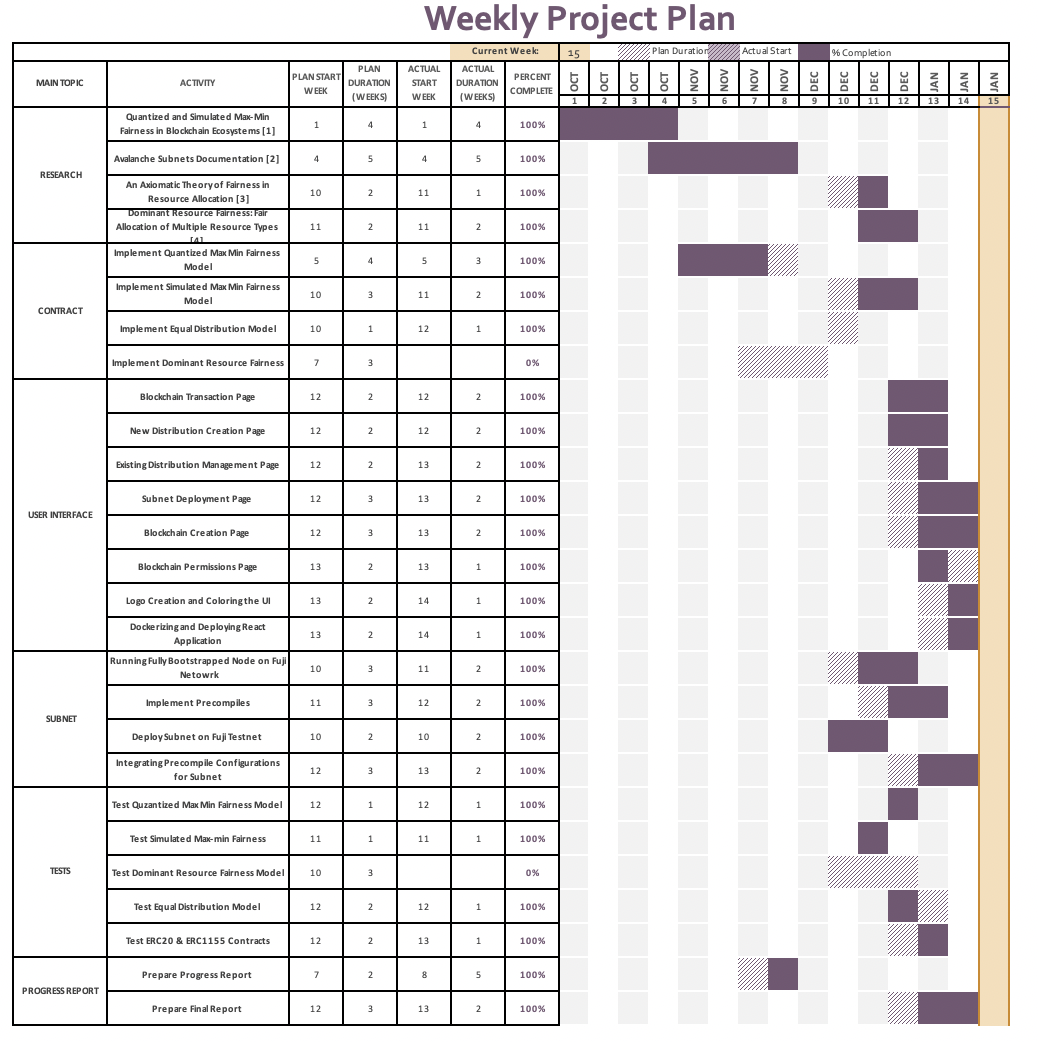
\includegraphics[width=1\textwidth]{weeklyplan.png}
	\caption{Weekly Plan}
\end{figure}

\begin{figure}[H]
	\centering
	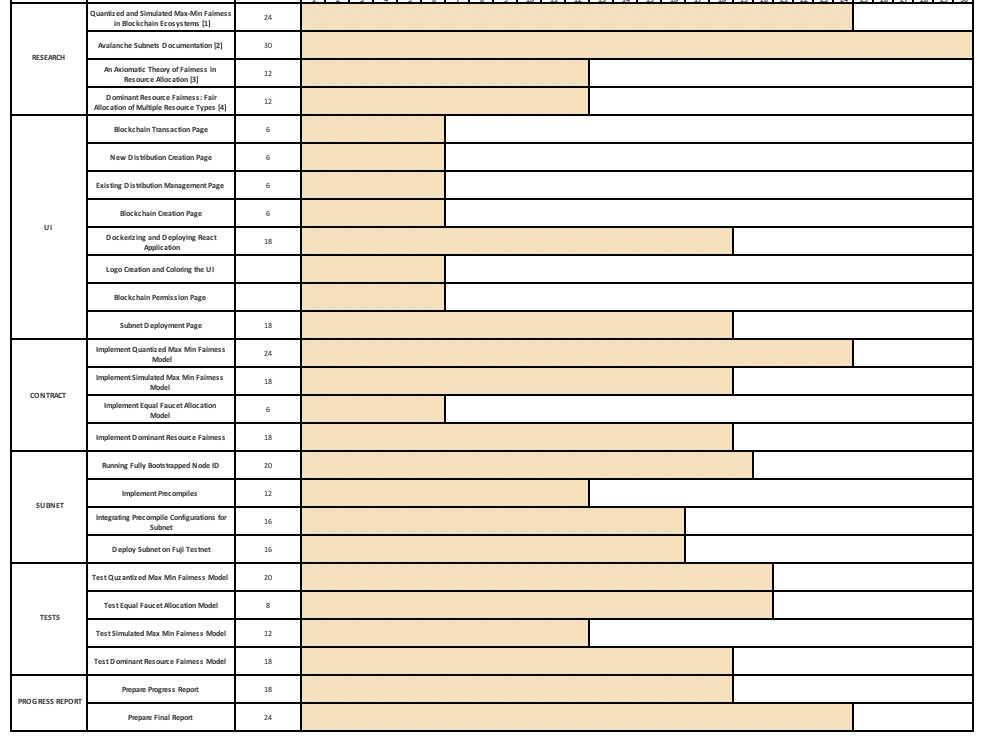
\includegraphics[width=1\textwidth]{time.png}
	\caption{Time and Resource Estimation}
\end{figure}
\subsection{Success Criteria}
The first criterion is completing tasks in obedience to the planned timeline. Since we continue cumulatively and future tasks depend on the previous ones, delivering both micro and macro tasks in time is substantial. 

Another success pointer is passing all the test cases. Tests are crucial in blockchain development since the contracts are immutable, and a small bug can have significant and undesirable consequences on monetary systems. As yet, we have implemented 35+ test cases which have all passed. As we add new functionalities to the contract, the number of test cases will increase.

The third criterion has a working subnet entirely deployed on Fuji Testnet. We officially release our product by deploying a contract to a public blockchain. So, anyone can check the fairness and transparency of the model.

\subsection{Risk Analysis}
Avalanche introduced its subnets concept very recently, in mid 2022s. Since that time, they have been making progress on the Subnets concept. However, it is still in its early days, and some of its functionalities need to be more stable, and the documentations need to be corrected.
Due to these circumstances, we frequently communicate with the Avalanche team via Discord or open an issue on their GitHub repository to clarify the documentation and fix the bugs in the repositories.

Implementing a Subnet on a Fuji Testnet, one of the Avalanche Testnets, requires having at least one fully bootstrapped and running node locally or in a virtual machine. Since there are high requirements for running an Avalanche Node, such as 16 GiB of RAM and 1 TiB of storage which cannot be affordable by our computers, we searched for the instance prices on AWS and realized the high costs. For the time being, we decided to create a Subnet on a local network instead of Fuji Testnet.

\subsection{Team Work}
The development of blockchain necessitates utmost attention as the contracts are immutable on the network and generally entail significant value. Consequently, we carefully reviewed each other's work on most components.

During the project, one team member was responsible for front-end development and connecting it to the blockchain, while the other focused on contract creation, subnets, and the blockchain creation process. In the final three weeks, we held daily meetings to review each other's work and offer constructive feedback.

In addition to these efforts, we increased the frequency of meetings with our advisor, C. Ozturan, from bi-weekly to weekly. Based on our advisor's feedback, we made some significant changes to the project's implementation. Furthermore, we organized two meetings with our co-advisor, S. Metin, and received valuable feedback from him.

\chapter{RELATED WORK}
\section{Resource Distribution Methods}
\subsection{Quantized Max-min Fairness}
We mostly followed the paper \textit{"Quantized and Simulated Max-min Fairness in Blockchain Ecosystems"}[1] in our Quantized Max-min Fairness distribution method design and implementation. 

The paper introduces adaptations of the Max-min Fairness algorithm: Quantized Max-min Fairness, Simulated Max-min Fairness, and their weighted versions. Blockchain faucets are used to concrete these algorithms. The details of Max-min Fairness and Quantized Max-min Fairness algorithms can be found in sections \textit{4.1.1} and \textit{4.1.2}, respectively.

We primarily followed the Quantized Max-min Fairness algorithm as in the paper but changed some fields that are unsuitable for our preferred design structure. The paper uses a selector variable to record the previous epoch's demands. Only two epochs are traceable with that selector, and any demand not claimed in the next epoch is lost. Instead of using a selector variable, we introduced a unique approach with constant-sized arrays which allow users to claim their proposed demands within a predefined demand expiration time. The details of this approach are explained in section \textit{6.2.1.3}.

\subsection{Simulated Max-min Fairness}
Simulated Max-min Fairness calculates the maximum available share that a system can offer to each user without exceeding capacity.
\newpage
While Quantized Max-min Fairness limits the demand volumes to a specific interval. However, a large number of users can make a demand for the resource. Simulated Max-min Fairness restricts the number of demanders but allows different weighting policies. 

The paper  \textit{"Quantized and Simulated Max-min Fairness in Blockchain Ecosystems"}[1]  compares Simulated Max-min Fairness to conventional Max-min Fairness algorithm and finds Simulated Max-min Fairness to be more affordable in terms of gas expenditures. 

\subsection{Dominant Resource Fairness}
The Paper \textit{"Dominant Resource Fairness: Fair Allocation of Multiple Resource Types"}[2] introduces Dominant Resource Fairness, a unique solution to the problem of fair distribution of resources in a system containing different types of resources. This algorithm is a generic adaptation of the Max-min Fairness model for multiple resource systems. 

A user's dominant share is the maximum share among all their shares. DRF computes the dominant share for each resource and each user. Then it simply applies Max-min Fairness to dominant shares. 

Paper demonstrates the traits of the Dominant Resource Fairness algorithm [2]: It is share-guaranteed, which means users can get at least 1/n (n denotes the number of users) of one resource. It is strategy-proof, meaning users would not be in a better position if they demanded more than they needed and had no reasons to lie about their resource usage. It is envy-free, which means no users prefer to get another user's share and would not be in a better position by taking it. It is also Pareto efficient [3], which means it is only possible for a user to get more resources by decreasing another user's resources.
Consequently, Dominant Resource Fairness [2] performs better than the other approaches, and we plan to add it to our distribution mechanism list.

\section{Avalanche Subnets}
\subsection{Avalanche Documentation}
We followed Avalanche's official documentation and GitHub repository to build our customized Subnet. The documentation is well-categorized, starting from explaining "Why we need to use a Subnet" to "Customizing a virtual machine for your Subnet." 
The Avalanche Documentation provides various ways of building and deploying a Subnet. These methods allow us to create our Subnet in a local network for development purposes and save us from challenging node running operations which require 50+ hours of bootstrapping times and over 1TiB of storage. If you want to deploy your Subnet to Fuji Testnet, Avalanche provides two unique command line interface solutions: Avalanche CLI and Subnet CLI. Avalanche CLI is a command line tool that allows us to access Avalanche's all facilities, especially on developing test Subnets. On the other hand, Subnet CLI is another tool for managing Subnets. They both serve the same purposes, using different commands. More explanation on Avalanche Subnets can be found in section \textit{4.2.2}. 

We have been following the guide using Subnet CLI. First, to create a blockchain on the to-be-created Subnet, we created a virtual machine based on the Subnet-EVM. Second, some validator nodes were added to Avalanche's primary network, which will be added to the Subnet later. Third, a Subnet is generated, and the previous nodes are added to the Subnet. Finally, a blockchain is created on the Subnet with the virtual machine created in the first step. The documentation also provides different kinds of solutions to customize a Subnet according to your applications' needs. These ways include using Genesis files, precompiles, chain configs, and upgrade configs which are explained in detail in section \textit{4.2.2.1}. We have also run into some difficulties. There were and are bugs and incorrect steps in these documentations, which congested and is still congesting us. We contacted the Avalanche team on Discord and opened several issues on GitHub to fix the repository. Because these updates take some time, we were able to progress more slowly than we should have.

\chapter{METHODOLOGY}
\section{Disribution Policies}
\subsection{Max-min Fairness}
Max-min fairness algorithm aims to maximize the minimum share distributed to users without wasting any capacity. 
Max-min fairness allocates resources to users in increasing order of their demand volume. Users are allocated at most what they request. For each user, the max-min fairness algorithm allocates the minimum of what the user asked for and the maximum amount they can get, total capacity divided by the number of demanders. This process is repeated until all the capacity is allocated or satisfies the users with their requested demand volume.
For example, let D be the set of demands, D = {2, 3.1, 3.5, 4, 6}, and let C be the capacity, C = 15. In the first iteration, we divide all the capacity by the number of demands. In this case, 15 / 5 = 3. Since this is larger than what the first demander has requested, this leaves 3 - 2 = 1 capacity left to be distributed among other demanders. The left capacity gives 1 / 4 = 0.25 resources to other demands. So, other demands get 3 + 0.25 = 3.25 resources. Since this is larger than the second demander has requested with an excess of 0.15 capacity, the excess capacity is distributed among other demanders again. This gives 0.15 / 3 = 0.05 capacity to each of the other demands, so the other demands get 3.25 + 0.05 = 3.3 capacity. Since this is lower than what other demanders requested, in the fair allocation, the first demander will get 2, the second demander  will get 3.1, and the other demanders will get 3.3 resources each.
\newpage
\subsection{Quantized Max-min Fairness}
The quantized max-min fairness algorithm[1] is a modified version of the max-min fairness algorithm where the number of demands for each demand volume is tracked, and the share calculation is made according to demand counts instead of the demands themselves. When a user makes a demand, the demand array is updated by incrementing the number of demands in the location corresponding to the relevant demand volume.
The share calculation function iterates over the demand array. It calculates the necessary capacity for each demand volume and compares it with the predetermined maximum capacity. If the necessary capacity is larger than the predetermined maximum capacity, the share calculation is stopped, and the previous demand volume is returned as the maximum share.
The necessary capacity is calculated based on the below formula for the to-be-determined maximum share value or proposal p (1<= p <= q, p,q E Z) is:
\begin{figure}[H]
\[
\sum_{i=1}^{p-1} i \cdot d_{i} + \sum_{j=p}^{q} p \cdot d_{j}
\]
\[
=\sum_{i=1}^{p-1} i \cdot d_{i} + p \cdot \sum_{j=p}^{q} d_{j}
\]
\[
=\sum_{i=1}^{p-1} i \cdot d_{i} + p \cdot (D - \sum_{i=1}^{p-1} d_{i})
\]
\caption{Formula for calculating total necessary capacity.}
\end{figure}

\newpage

Where \textit{\textrm{d}\textsubscript{i}} is the \textit{\textrm{i}\textsuperscript{th}} element of the demand array and \textit{D} is the total number of demands. In the final formula, left side of the plus sign, \textit{i $\cdot$ \textrm{d}\textsubscript{i}}  stands for the total capacity reserved based on the selected \textit{i} value in that iteration, and the right side of the plus sign stands for the leftover demands, \textit{(total number of demands - satisfied demands with selected i) $\cdot$ selected maximum proposal i}. The summation of these two shows the necessary capacity. 


% Please add the following required packages to your document preamble:
% \usepackage[table,xcdraw]{xcolor}
% If you use beamer only pass "xcolor=table" option, i.e. \documentclass[xcolor=table]{beamer}
% Please add the following required packages to your document preamble:
% \usepackage[table,xcdraw]{xcolor}
% If you use beamer only pass "xcolor=table" option, i.e. \documentclass[xcolor=table]{beamer}
\begin{table}[H]
	\begin{tabular}{|c|c|c|c|c|c|c|c|c|}
		\hline
		Demand Volume             & 1  & 2  & 3  & 4  & 5  & 6  & 7                                                          & 8  \\ \hline
		Number of Demands (NoD)   & 2  & 3  & 4  & 0  & 1  & 2  & 2                                                          & 2  \\ \hline
		Total Demand Volume (TDV) & 2  & 6  & 12 & 0  & 5  & 12 & 14                                                         & 16 \\ \hline
		Cumulative NoD            & 2  & 5  & 9  & 9  & 10 & 12 & 14                                                         & 16 \\ \hline
		Cumulative TDV            & 2  & 8  & 20 & 20 & 25 & 37 & 51                                                         & 67 \\ \hline
		Necessary Capacity        & 15 & 28 & 38 & 44 & 50 & 55 & \cellcolor[HTML]{34FF34}{\color[HTML]{000000} \textbf{58}} & 67 \\ \hline
	\end{tabular}
\\
\centering\caption{Example of QMF}
\end{table}


In the example above, the maximum demand volume is set to 8, which means users can demand a maximum of 8 units. The demand set \textit{D} is \textit{[1, 1, 2, 2, 2, 3, 3, 3, 3, 5, 6, 6, 7, 7, 8, 8]} and for the sake of example, the maximum proposed capacity is selected as 60. The number of demands (NoD) shows the number of users that requested that demand volume. More clearly, it represents that two users demanded 1 unit, three users demanded 2 units, and so on. Total demand volume, \textit{TDV}, is the multiplication of a demand volume and the number of demands. Their cumulative sums are also given in the table. The last line of the table, the necessary capacity, is calculated by the above formula.

The capacity was set to 60 for this example. Hence, the returning value, maximum share, will be 7, corresponding to the maximum necessary capacity value of 58, which is lower than 60.

\section{Tools Used}
\subsection{Solidity}

Smart contracts are the code blocks that run on the blockchain. These code blocks, composed of some functions and state variables, are deployed to the blockchain and can be called by submitting a transaction to the network. Smart contracts are written in high-level programming languages such as Solidity to be compiled down to Ethereum Virtual Machine (EVM) bytecodes. 

Solidity is an object-oriented programming language for generating smart contracts to be executed on EVM or EVM-compatible blockchain. Since Avalanche is an EVM and Solidity-compatible blockchain, we can use Solidity to write smart contracts for Avalanche blockchain. Additionally, Avalanche’s documentation is primarily written in Solidity, which encourages us to use Solidity to write smart contracts. 

\subsection{Hardhat}
Hardhat is an environment that helps developers to polish the smart contract development processes. Hardhat comes with a local Ethereum network specifically designed for development purposes, which allows us to compile, debug, test, and deploy our smart contracts on that local network. 

Another great thing about it is that the Hardhat toolbox also has a gas reporter plugin. That plugin gives information about how much gas is used in methods or deployments. 
\newpage
\subsection{Avalanche Subnets}
Scalability is one of the pillars of the blockchain trilemma. Different methods, like Ethereum's layer 2 solutions, are proposed to solve blockchains' scalability problems without harming decentralization and security. Subnets or sub-networks are the solutions proposed by Avalanche to the scalability problem.

Subnets are a set of validators that work together to reach a consensus on their blockchains. Depending on an application's purposes, membership system, and token economy model, a Subnet may define its own execution rules. 

For instance, a Subnet may restrict validators who did not pass the KYC check, or a Subnet may require specific Hardware features such as high CPU or large storage depending on the application's needs, or a Subnet may give permission only to predefined validators if the blockchain data wants to be kept private, only visible by the set of those predefined validators.

Subnets can deploy their blockchains by customizing parameters depending on the application's needs. Two ways of customizing blockchain are by formatting Genesis data or using Precompiles.

\subsection{Precompiles}
The Genesis file is a combination of the initial configuration of a Subnet and headers of the genesis block of to-be-created blockchain. Subnets can be customized depending on the needs of applications by changing variables in the Genesis file. 

In the Subnet Config code block, the chain ID represents the ID of the to-be-created chain. The Hardforks field allows Subnet owners to activate newly released protocols on Subnet by adding the configuration of the protocol to this field.

In the Fee Config code block, fee and block-related settings such as maximum gas consumption limit in a block, block production rate, and minimum base fee used by a transaction are adjustable. For instance, if the Subnet owner wants their network to be fast, transaction fees can be set high since higher transaction fees mean faster verification time.

In the Validator Fee Recipient code block, adjusting the fee recipients field true allows validators to be fee recipients.
In the Native Token Allocation code block, the addresses and their initial balances are defined. Since a transaction requires some fee to be executed, genesis allocation should be provided to interact with the to-be-created network.

In the Precompiles code block, various precompiled contracts can be enabled to add custom functionalities to Subnets. Some of these precompiles are explained below.

Contract Deployer Allow List Config precompile allows us to authorize addresses that can deploy contracts. In other words, admin addresses, which can deploy new contracts, are adjusted by giving a specific list of addresses as input to this precompile. 

Contract Native Minter Config precompile can be used to mint native assets in the Subnet. 

Tx Allow List Config precompile allows us to specify the addresses that can send a transaction to the network. For example, if the Subnet owner wants to make their network only usable by a private group of people, they can specify the allowed addresses.

Finally, Genesis Block headers contain generic blockchain parameters such as nonce, timestamp, gas limit, difficulty, coinbase, and parent hash to define Genesis Block.

\chapter{REQUIREMENTS SPECIFICATION}
\section{System Requirements}
The system requirements shall be examined in subsections according to the functionalities provided. The core functionalities that are provided by our system could be grouped according to their target user types: Admin User and Permissioned User. Our system shall both allow users to deploy their own customized subnets with their own fair distribution policies, and interact with the subnets that they are a member of by participating in the fair distribution mechanisms of those with demand and claim functionalities.

Before proceeding with the functionalities, it is a better approach to start with the definitions.

\subsection{Glossary}
\textbf{Admin User}: The user who deploys their customized Subnet on our platform, and has the authority on it. They can add Permissioned Users to allow them to transact on their Subnets.

\textbf{Distribution Algorithm}: An algorithm that can be used in order to distribute assets on a blockchain. It is implemented in smart contracts and it can be used for both distributing the native asset of the blockchain or tokens issued on it.

\textbf{Native Asset}:  The main asset of a blockchain that is used for paying the gas fees and transacting on the blockchain.

\newpage

\textbf{Permissioned User}: The user who is given permission to transact on a Subnet deployed by an Admin User. They have permission to interact with the contracts that are used to distribute resources, according to the fairness algorithm that they are deployed with. However, they may not have the authority to deploy contracts on the Subnet themselves, and may have access to limited functionality on it.

\textbf{Resource Distribution Contract}: A smart contract that has some assets and distributes them, according to its distribution algorithm, to the Permissioned Users who make demands.

\textbf{Subnet}: An independent network with a customizable underlying VM, permission settings, and tokenomics. Subnets are a new solution proposed by the Avalanche team. 

\textbf{User}: The person who comes to our platform to use any functionality, including both deploying a Subnet (and thus becoming the Admin of it) or interacting with any deployed Subnet if they have permission on it.

\subsection{Subnet Deployment}
\begin{itemize}
	\item [5.1.2.1]
	The system shall provide a dashboard for Users to deploy their own customized Subnets.
	\\
	\item [5.1.2.2.]
	The system shall take parameters from the User for the customization of their Subnets.
	\begin{itemize}
		\item [5.1.2.2.1.]
		The system shall provide the option to customize the Subnet’s native asset by asking the User for various parameters, including its ticker, supply, etc.
		\item [5.1.2.2.2.]
		The system shall provide the option to customize the permissions on the Subnet by taking a list of addresses from the User to give various permissions.
		\newpage
		\item [5.1.2.2.3.]
		The system shall allow the User to select their own distribution algorithm among the implemented choices for the distribution of the Subnet’s native asset.
		\item [5.1.2.2.4.]
		The system shall provide the option to customize the distribution algorithm by allowing the User to edit various parameters, including the epoch duration, maximum demandable quantity, and epoch capacity.
		\\
	\end{itemize}
	\item [5.1.2.3.]
	The system shall be able to generate the resource distribution contract according to the parameters provided by the User and deploy the Subnet.
	\\
	\item [5.1.2.4.]
	The system shall be able to complete the deployment of the Subnet requested by the User and make them the Admin User of it.
	\\
	\item [5.1.2.5.]
	The system shall also complete the deployment of the initial blockchain on the newly created Subnet.
\end{itemize}

\subsection{Subnet Management}
\begin{itemize}
	\item [5.1.3.1]
	Although the system shall not be focused on the Subnet’s management after it is deployed, it shall provide the Admin User with the necessary information like Subnet ID, Blockchain ID, permissioned addresses, the address of the native asset distribution contract, etc. when the Subnet is available.
	\\
	\item [5.1.3.2.]
	The system shall provide a Subnet Management dashboard for the Admin Users in which the information related to the Subnets created by them is shown.
	\\
	\item [5.1.3.3.]
	Admin Users shall be able to deploy additional resource distribution contracts using this Subnet Management dashboard.
\end{itemize}

\subsection{Deploying Additional Resource Distribution Contracts on Subnets}
\begin{itemize}
	\item [5.1.4.1]
	The system shall allow Admin Users to deploy more resource distribution contracts that could be used to allocate resources other than the native asset of the Subnet.
	\\
	\item [5.1.4.2.]
	The system shall allow the customization of these contracts with the similar options provided for the Subnet native asset distribution contract.
	\\
	\item [5.1.4.3.]
	The system shall allow the Admin Users to deploy resource distribution contracts that distribute multiple resources at the same time using the DRF algorithm, or an independent implementation of the Quantized Max-min Fairness algorithm [1] for each resource.
	\\
	\item [5.1.4.4.]
	The system shall allow the Admin User to use either the ERC-20 or ERC-1155 standard to represent the resources in the blockchain, depending on their needs.
\end{itemize}

\subsection{Subnet Interactions}
\begin{itemize}
	\item [5.1.5.1]
	The system shall provide an interface to access any Subnet with its ID.
	\\
	\item [5.1.5.2.]
	The system shall allow any Permissioned User to make demands for the available resources on the Subnet by interacting with the resource distribution contracts.
	\\
	\item [5.1.5.3.]
	The system shall allow any Permissioned User to claim their shares after the epoch that they made a demand ends, before the expiration time.
	\\
	\item [5.1.4.4.]
	The system shall provide an option for claiming pending shares in bulk, with a single transaction.
\end{itemize}

\section{System Architecture}

\subsection{UML Use Case Diagram}
The use cases provided by the system are basically explained in the UML Use Case Diagram below. The functionalities are grouped according to the aforementioned user types and the inheritance relationship between them.

\begin{figure}[H]
	\centering
	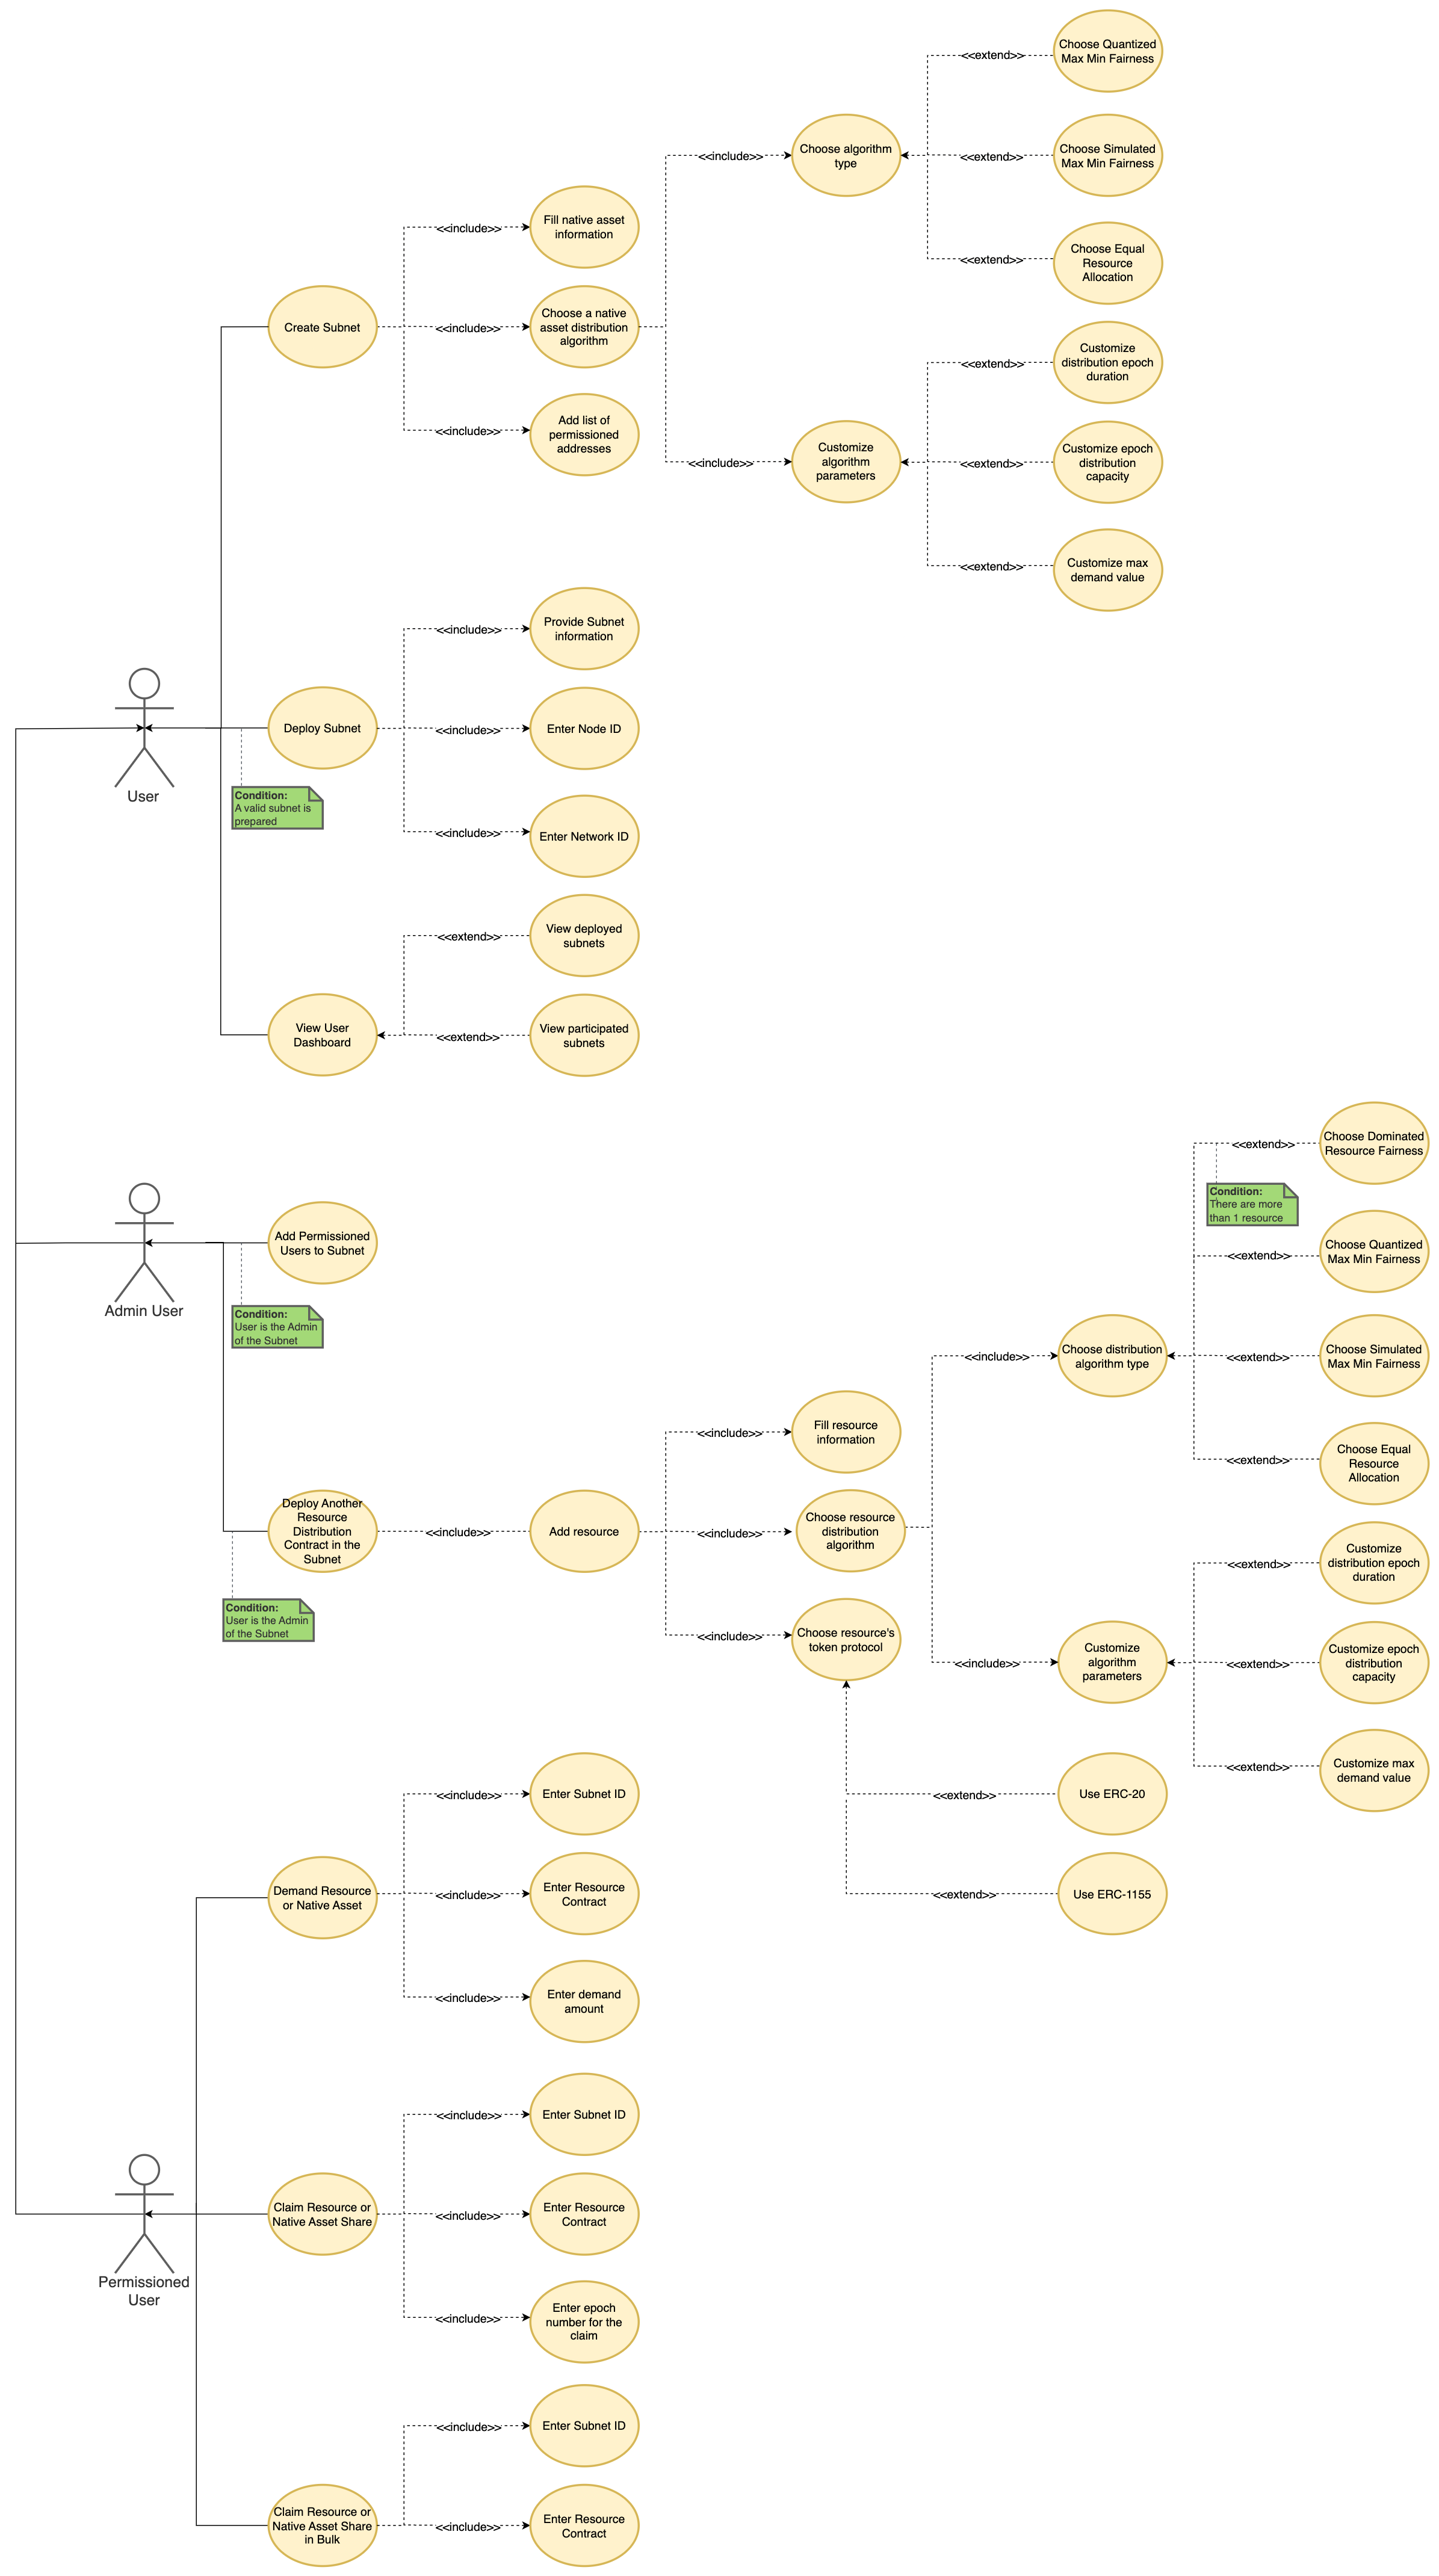
\includegraphics[width=0.6\textwidth]{use-case-big.png}
	\caption{UML Use Case Diagram}
\end{figure}

\chapter{DESIGN}

\section{Information Structure}
The Entity-Relationship Diagram below shows the relationships between the components of the platform and the blockchain elements.

\begin{figure}[H]
\centering
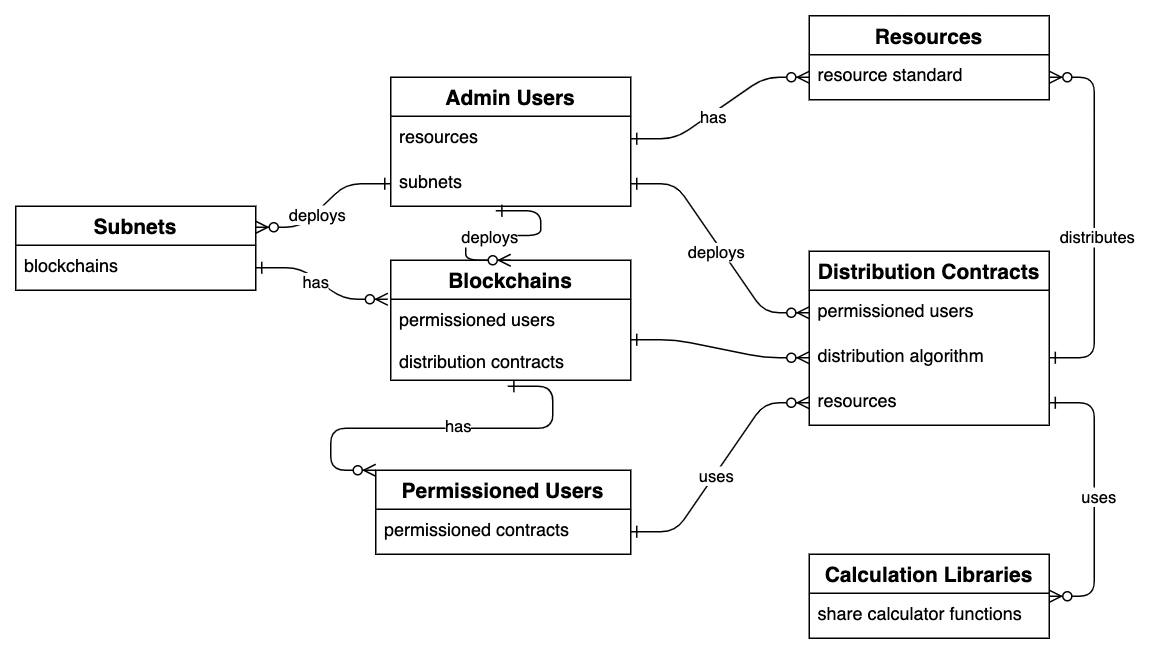
\includegraphics[width=1\textwidth]{erdiagram2.png}
\caption{Entity-Relationship Diagram}
\end{figure}

\section{Information Flow}
As mentioned in the Requirements, the fundamental functionalities provided by our system may be observed from the different perspectives of the deployer and the users of the Subnet, namely the Admin User and Permissioned Users. These fundamental functionalities in the system have been modeled using flowcharts and functional block diagrams.

\subsection{Flowcharts}
Firstly, two fundamental functionalities of an Admin User are summarized: deploying a subnet and deploying additional resource distribution contracts on a subnet. 

In \textit{Figure 6.2}, the deployment of a subnet is explained. The deployment process consists of two phases, namely, the Creation and the actual Deployment of it. The steps are explained below:
\begin{itemize}
	\item [1.]
	The Admin User first provides the information related to the subnet. These pieces of information may include subnet’s name, the native asset’s name and ticker, and some parameters that set the permissions on it.
	\\
	\item [2.]
	The parameters related to the distribution of the native asset of the Subnet are provided. Those will determine how the distribution of the main resource will be made on this newly created subnet.
	\\
	\item [3.]
	The subnet creation process is completed at this step. If the provided information is valid, then the deployment part starts.
	\\
	\item [4.]
	The Admin User provides some node information that belongs to the nodes that will be validating the subnet. Without validators, the deployment may not be completed.
	\\
	\item [5.]
	If the node information is also valid, the deployment is completed and the Admin User will see the Subnet ID and Blockchain ID information of their deployed subnet.
\end{itemize}

\newpage

In \textit{Figure 6.3}, on the other hand, the Admin User tries to deploy additional resource distribution contracts on an existing subnet. For this process to succeed, they will need a healthy subnet that is being validated by the nodes provided in the subnet deployment process and the ID of the blockchain on it. The steps for this process can be viewed below:
\begin{itemize}
	\item [1.]
	The Admin User first provides the information related to their subnet and the blockchain on it by entering their ID. If the subnet is healthy on the given ID, the process continues.
	\\
	\item [2.]
	The second check is made to determine whether the Admin User has the authority on the subnet entered.
	\\
	\item [3.]
	After the checks on Steps 1 \& 2, the system takes the parameters that will determine the distribution of this new resource. These parameters may include the name, ticker, and underlying protocol (ERC-20 or ERC-1155) of this resource. Additionally, the input that will customize the resource distribution contract are also taken from the user, like the distribution algorithm and the distribution parameters.
	\\
	\item [4.]
	If the parameters provided are also valid, then the system directs the transaction to the Admin User’s wallet, and then to the subnet’s blockchain. If the transaction is successful, the deployment is completed. Otherwise, the Admin User will see the error message related to the transaction.
\end{itemize}

\begin{figure}[H]
	\centering
	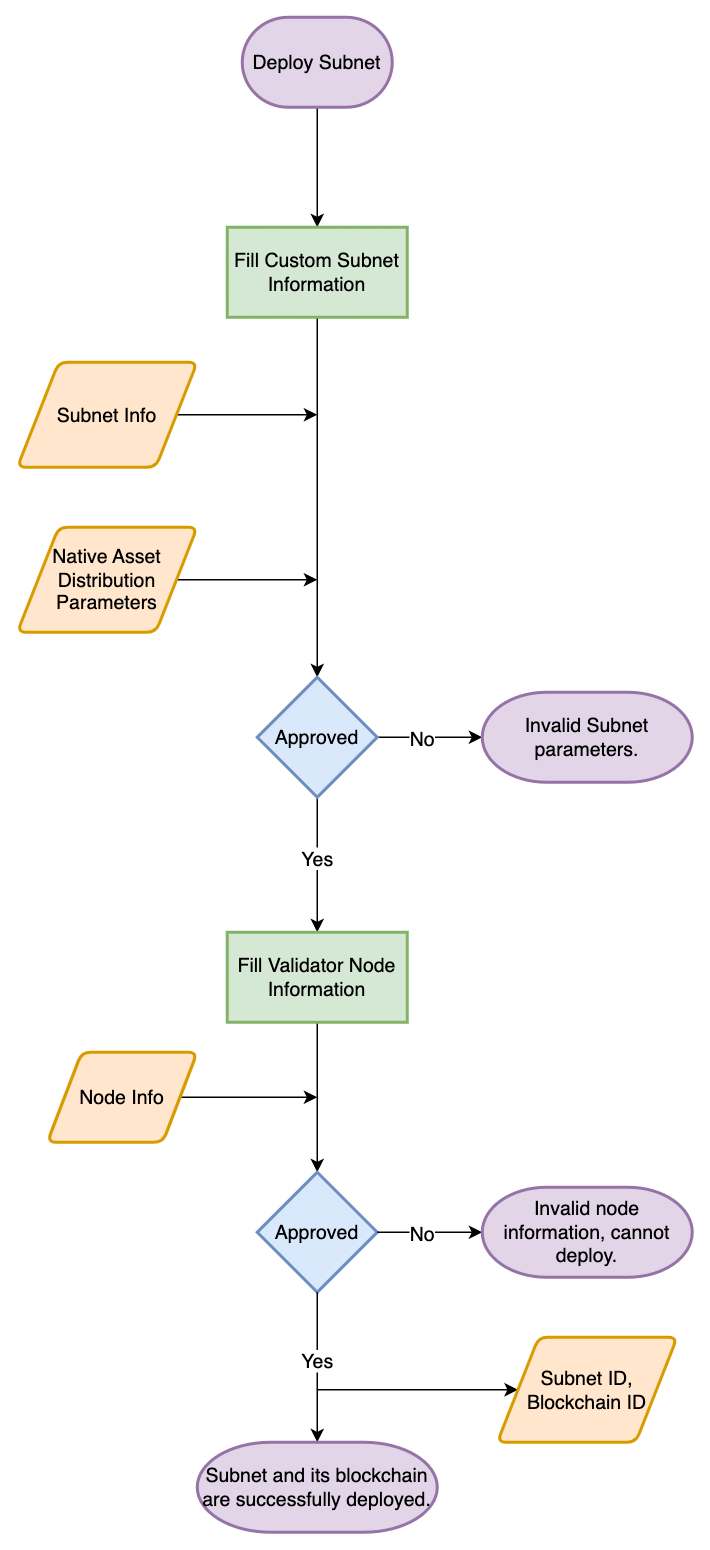
\includegraphics[width=0.5\textwidth]{flow1.png}
	\caption{Flowchart for Subnet Deployment
	}
\end{figure}
\begin{figure}[H]
	\centering
	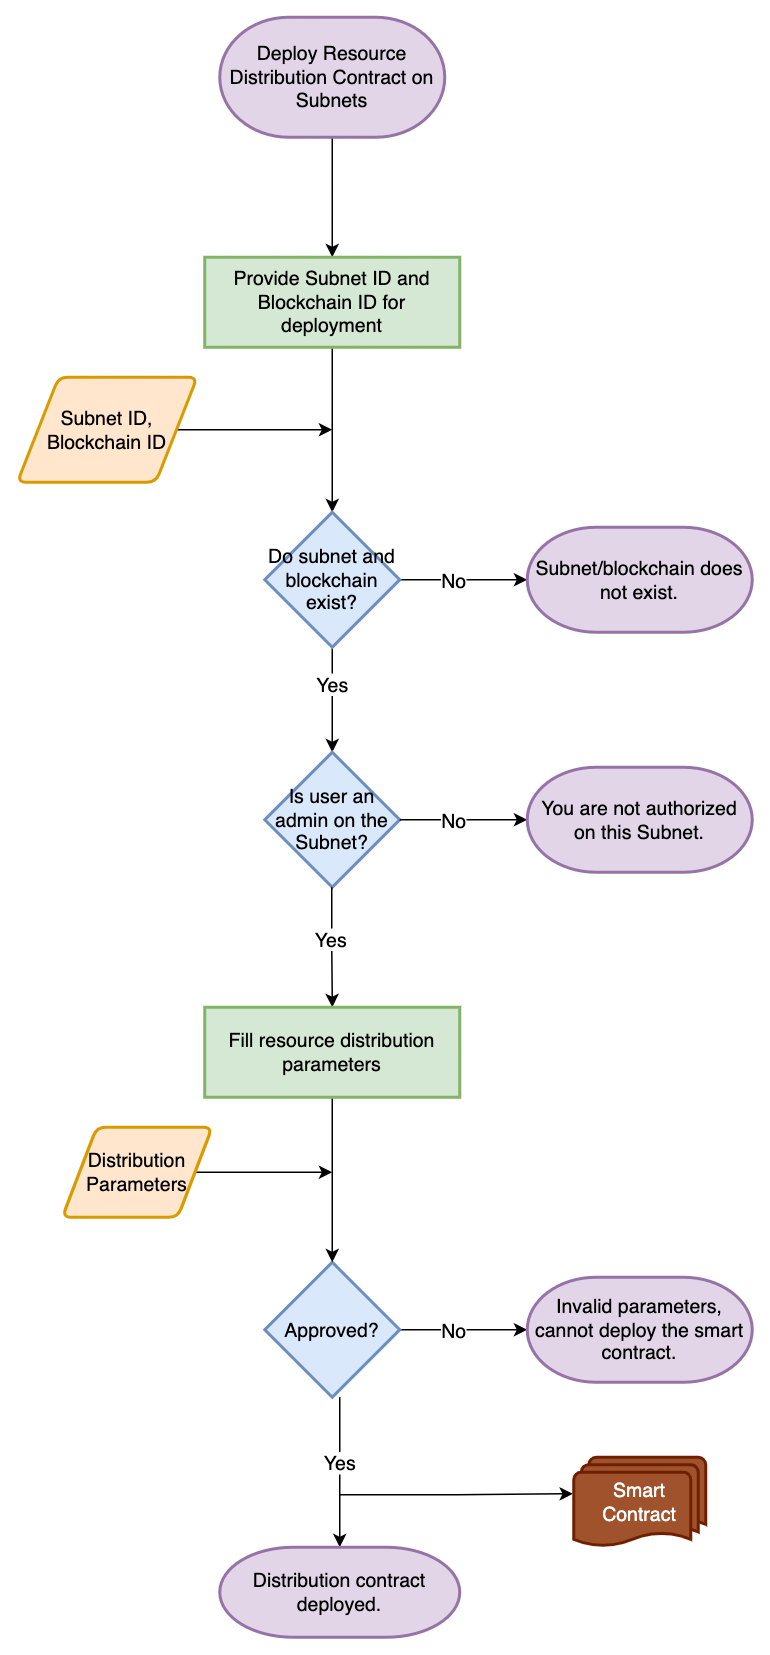
\includegraphics[width=0.5\textwidth]{flow2.png}
	\caption{Flowchart for Resource Distribution Contract}
\end{figure}

In the last two diagrams, the demand and claim processes of the Permissioned User are summarized.

In \textit{Figure 3}, the demand steps are shown for a Permissioned User. The explanation for those can be followed below:
\begin{itemize}
	\item [1.]
	The User first provides the information related to the subnet and the blockchain on it and the resource that they want to demand. If the information provided is correct, the process continues.
	\\
	\item [2.]
	The User needs to be permissioned on the given subnet. The process fails otherwise.
	\\
	\item [3.]
	At this step, the contract call is made with the demand volume that the Permissioned User provides. The process is terminated according to the result of the contract call.
	\\
	\item [4.]
	Please note that the validity of the Permissioned User’s demand is checked according to multiple criteria in the smart contract, and those are not included in the flowchart. These criteria may also vary depending on the distribution algorithm of the resource.
\end{itemize}

In \textit{Figure 4}, the User tries to claim their share from a previous epoch.
\begin{itemize}
	\item [1.]
	The User first provides the information related to the subnet and the blockchain on it and the resource that they want to demand. If the information provided is correct, the process continues.
	\\
	\item [2.]
	The User needs to be permissioned on the given subnet. The process fails otherwise.
	\\
	\item [3.]
	Then, the Permissioned User provides the epoch number that they would like to claim their share. If they do not have such a pending share, the process fails.
	\\
	\item [4.]
	After these checks, the contract call is made with the claim epoch number that the Permissioned User provides. The process is terminated according to the result of the contract call.
\end{itemize}

\begin{figure}[H]
	\centering
	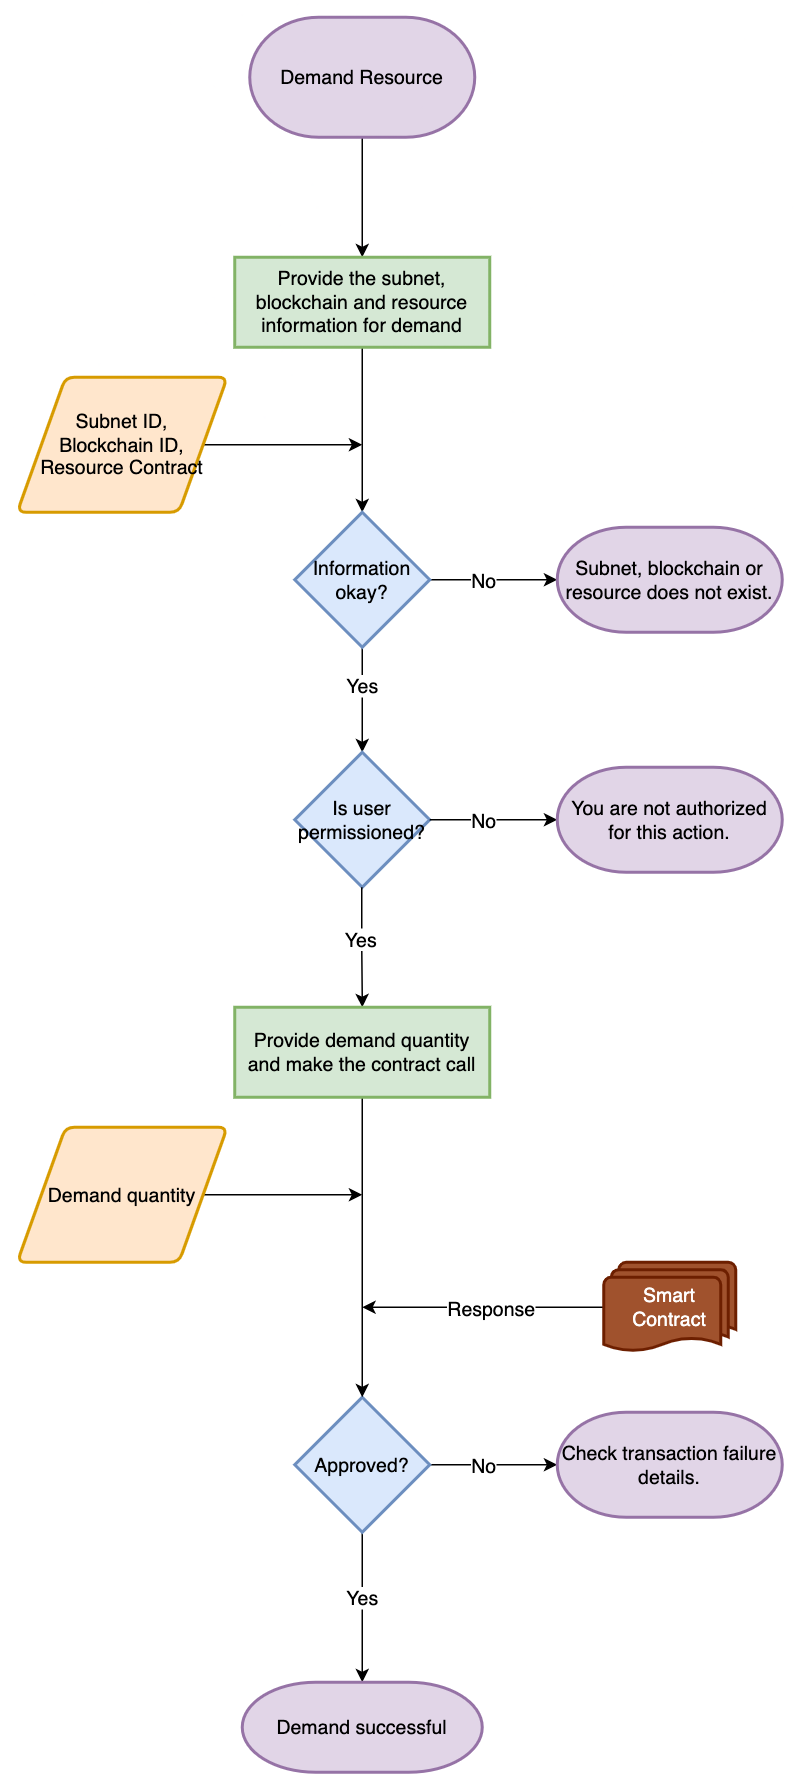
\includegraphics[width=0.5\textwidth]{flow3.png}
		\caption{Flowchart for Demand}
\end{figure}
\begin{figure}[H]
	\centering
	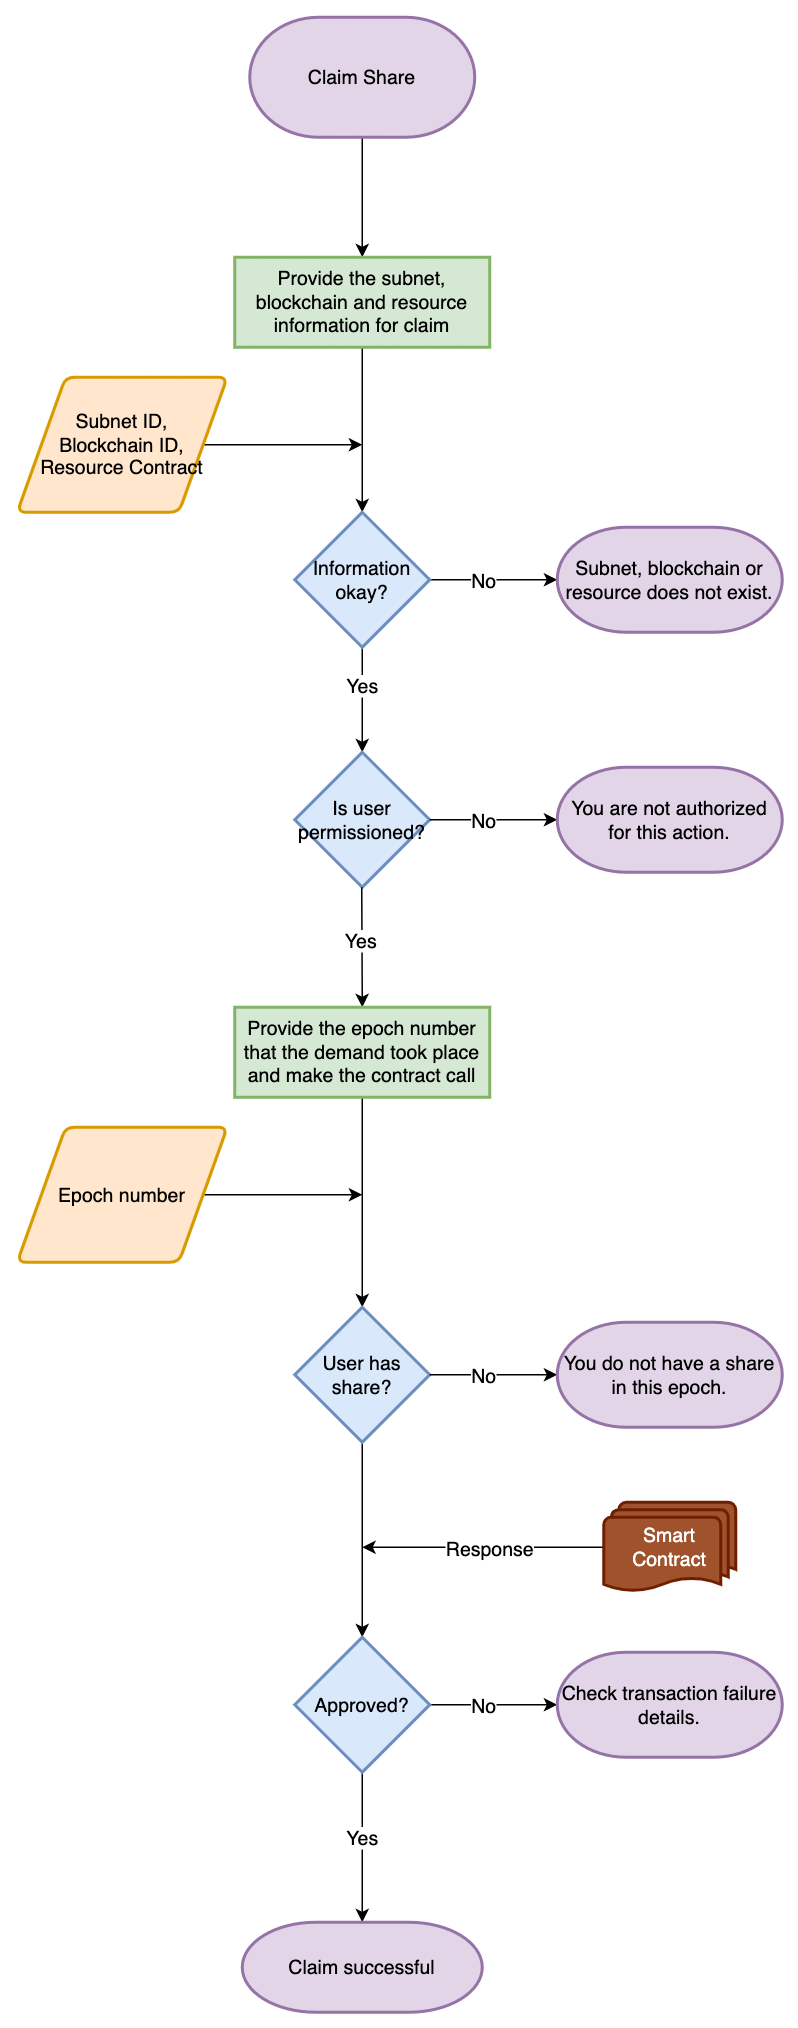
\includegraphics[width=0.5\textwidth]{flow4.png}
	\caption{Flowchart for Claim}
\end{figure}

\subsection{Functional Flow Block Diagrams}
In this subsection, the functionalities explained with the flowcharts are put together and the input and output parameters of those are provided in a more detailed way using the functional flow block diagrams. The flow for both user type’s functions can be observed in the related diagrams.

\begin{figure}[H]
	\centering
	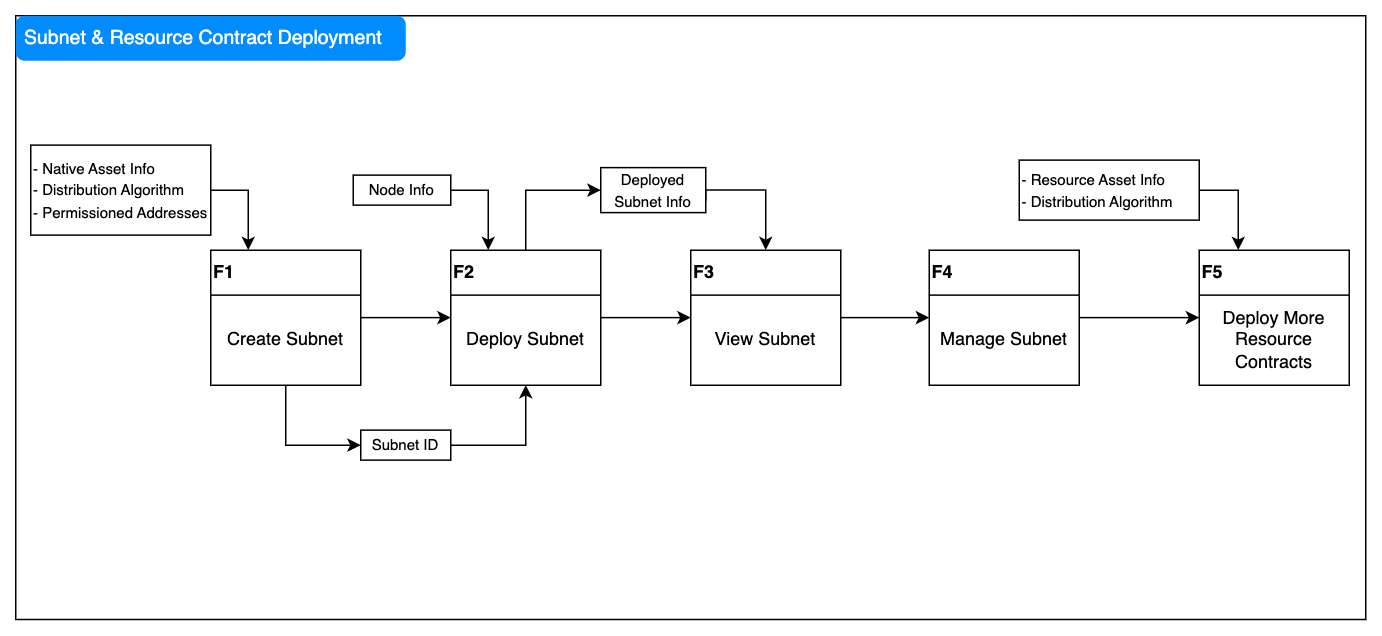
\includegraphics[width=1\textwidth]{function_1.png}
	\caption{Subnet \& Resource Contract Deployment}
\end{figure}

\begin{figure}[H]
	\centering
	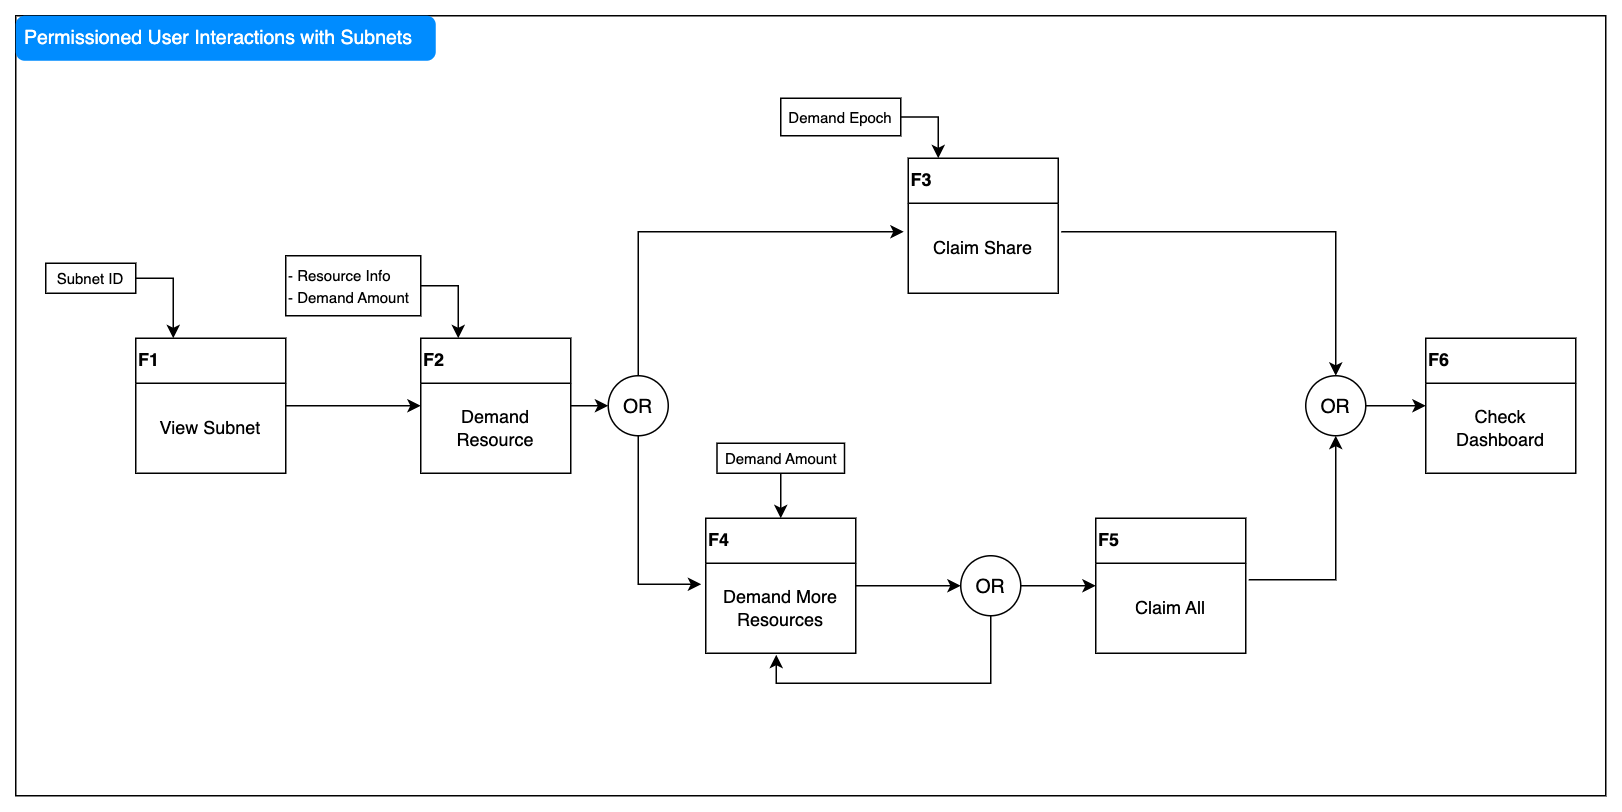
\includegraphics[width=1\textwidth]{function_2.png}
	\caption{Permissioned User Interactions with Subnets}
\end{figure}

\section{Systen Design}
\subsection{Contract \& Subnet Structure}
\subsubsection{Permissioned Subnet Structure}
In our system, we will provide the Admin Users with the opportunity to restrict the usage of their subnets. The subnets created by using our system will be permissioned by default, and only the list of addresses provided by the Admin User will be allowed to transact on the subnet and interact with the distribution contracts. The system will show the options to restrict access to interactions with some distribution contracts, custom contract deployment, and even transacting on the subnet in general. 

This kind of subnet structure prevents fair distribution methods from being abused by users who make multiple demands in a single epoch using multiple wallets. 

\begin{figure}[H]
	\centering
	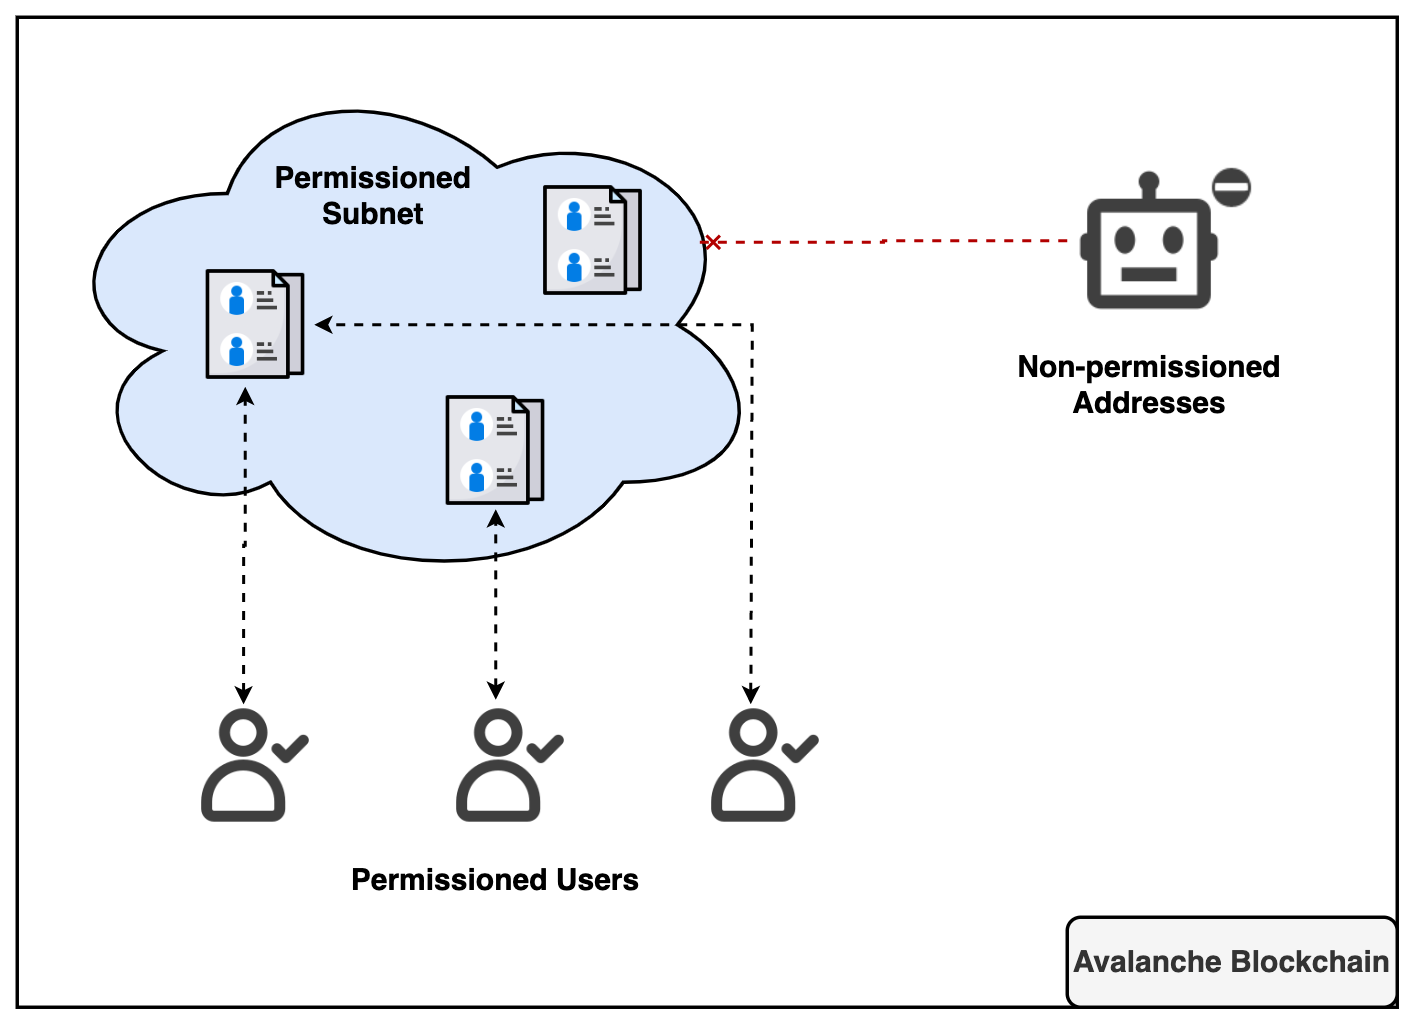
\includegraphics[width=1\textwidth]{precompile_1.png}
	\caption{Permissioned Subnet Structure}
\end{figure}

\subsubsection{Relationship Between Resources}
There are fundamentally two main kinds of assets in blockchains. The first one is the blockchain’s native asset that can be used to pay the gas fees and provide utilities on the base level. The second one is the non-native assets that are issued on the blockchain thanks to the utility provided by the native asset. These non-native assets may follow some common token standards like ERC-20, ERC-1155, and ERC-721.

In our system, the fair distribution methods we provide could be used for both distributing native assets and non-native assets representing additional resources in a community. 
\newpage
A newly created subnet’s native asset distribution contract can be deployed at the genesis of the subnet, utilizing the precompiles. Then, the subnet’s native asset could be emitted from this contract with a fair algorithm. 

As mentioned, other resources represented with the common token standards could also be distributed from the smart contracts deployed on the existing subnet, easily. The same permission requirements, or even more limited ones, could be applied to restrict access to these additional resources.

The relationship between the native asset and the non-native assets is shown in \textit{Figure 6.9}. The native asset empowers the subnet itself and is needed to deploy more resources on the network. With that said, the native asset itself is also distributed fairly, as can be seen in the figure.

\begin{figure}[H]
	\centering
	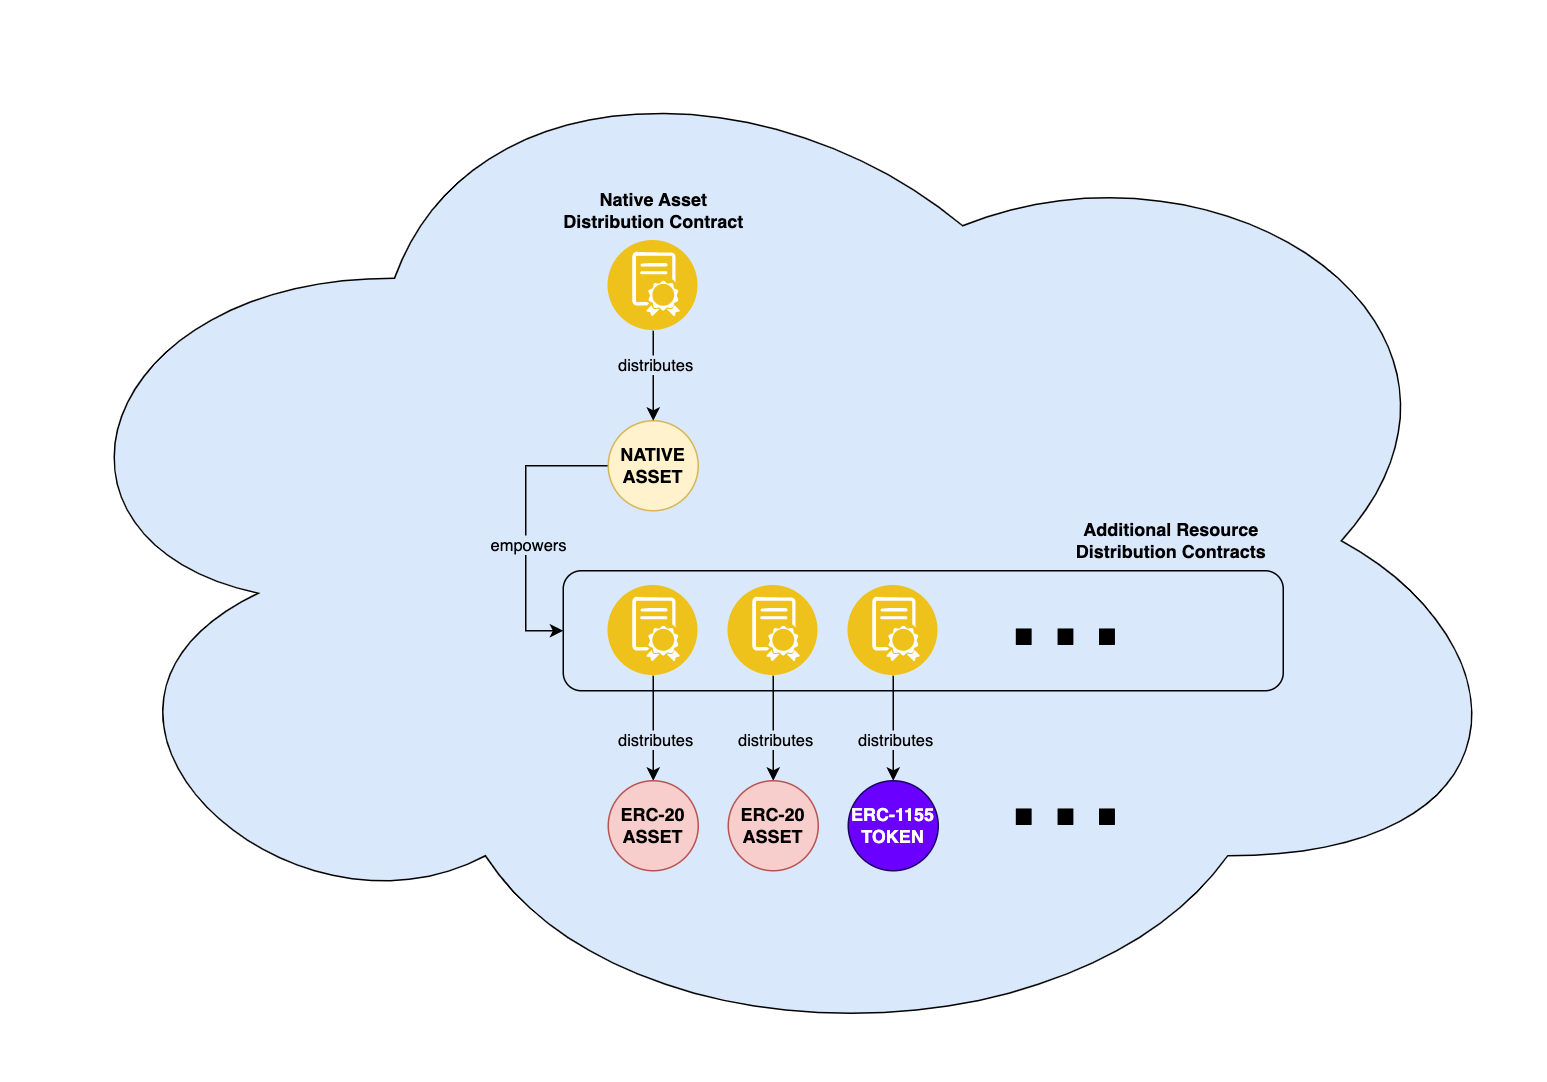
\includegraphics[width=1\textwidth]{subnet_2.png}
	\caption{Resource Distribution Contracts in a Subnet}
\end{figure}

Apart from those, it is possible for a single resource distribution contract to distribute more resources. These contracts may use the same distribution algorithms as the ones used for the distribution of the native assets, implemented separately for each resource, or use another detailed algorithm that we will introduce named Dominant Resource Fairness [2]. 

An example of a smart contract that could be used for distributing multiple resources can be seen in \textit{Figure 6.9}.

\subsubsection{The Class Structure of the Distribution Contracts Represented with UML}
In \textit{Figure 6.10}, the class structure of the distribution contracts are represented with UML.
\begin{figure}[H]
	\centering
	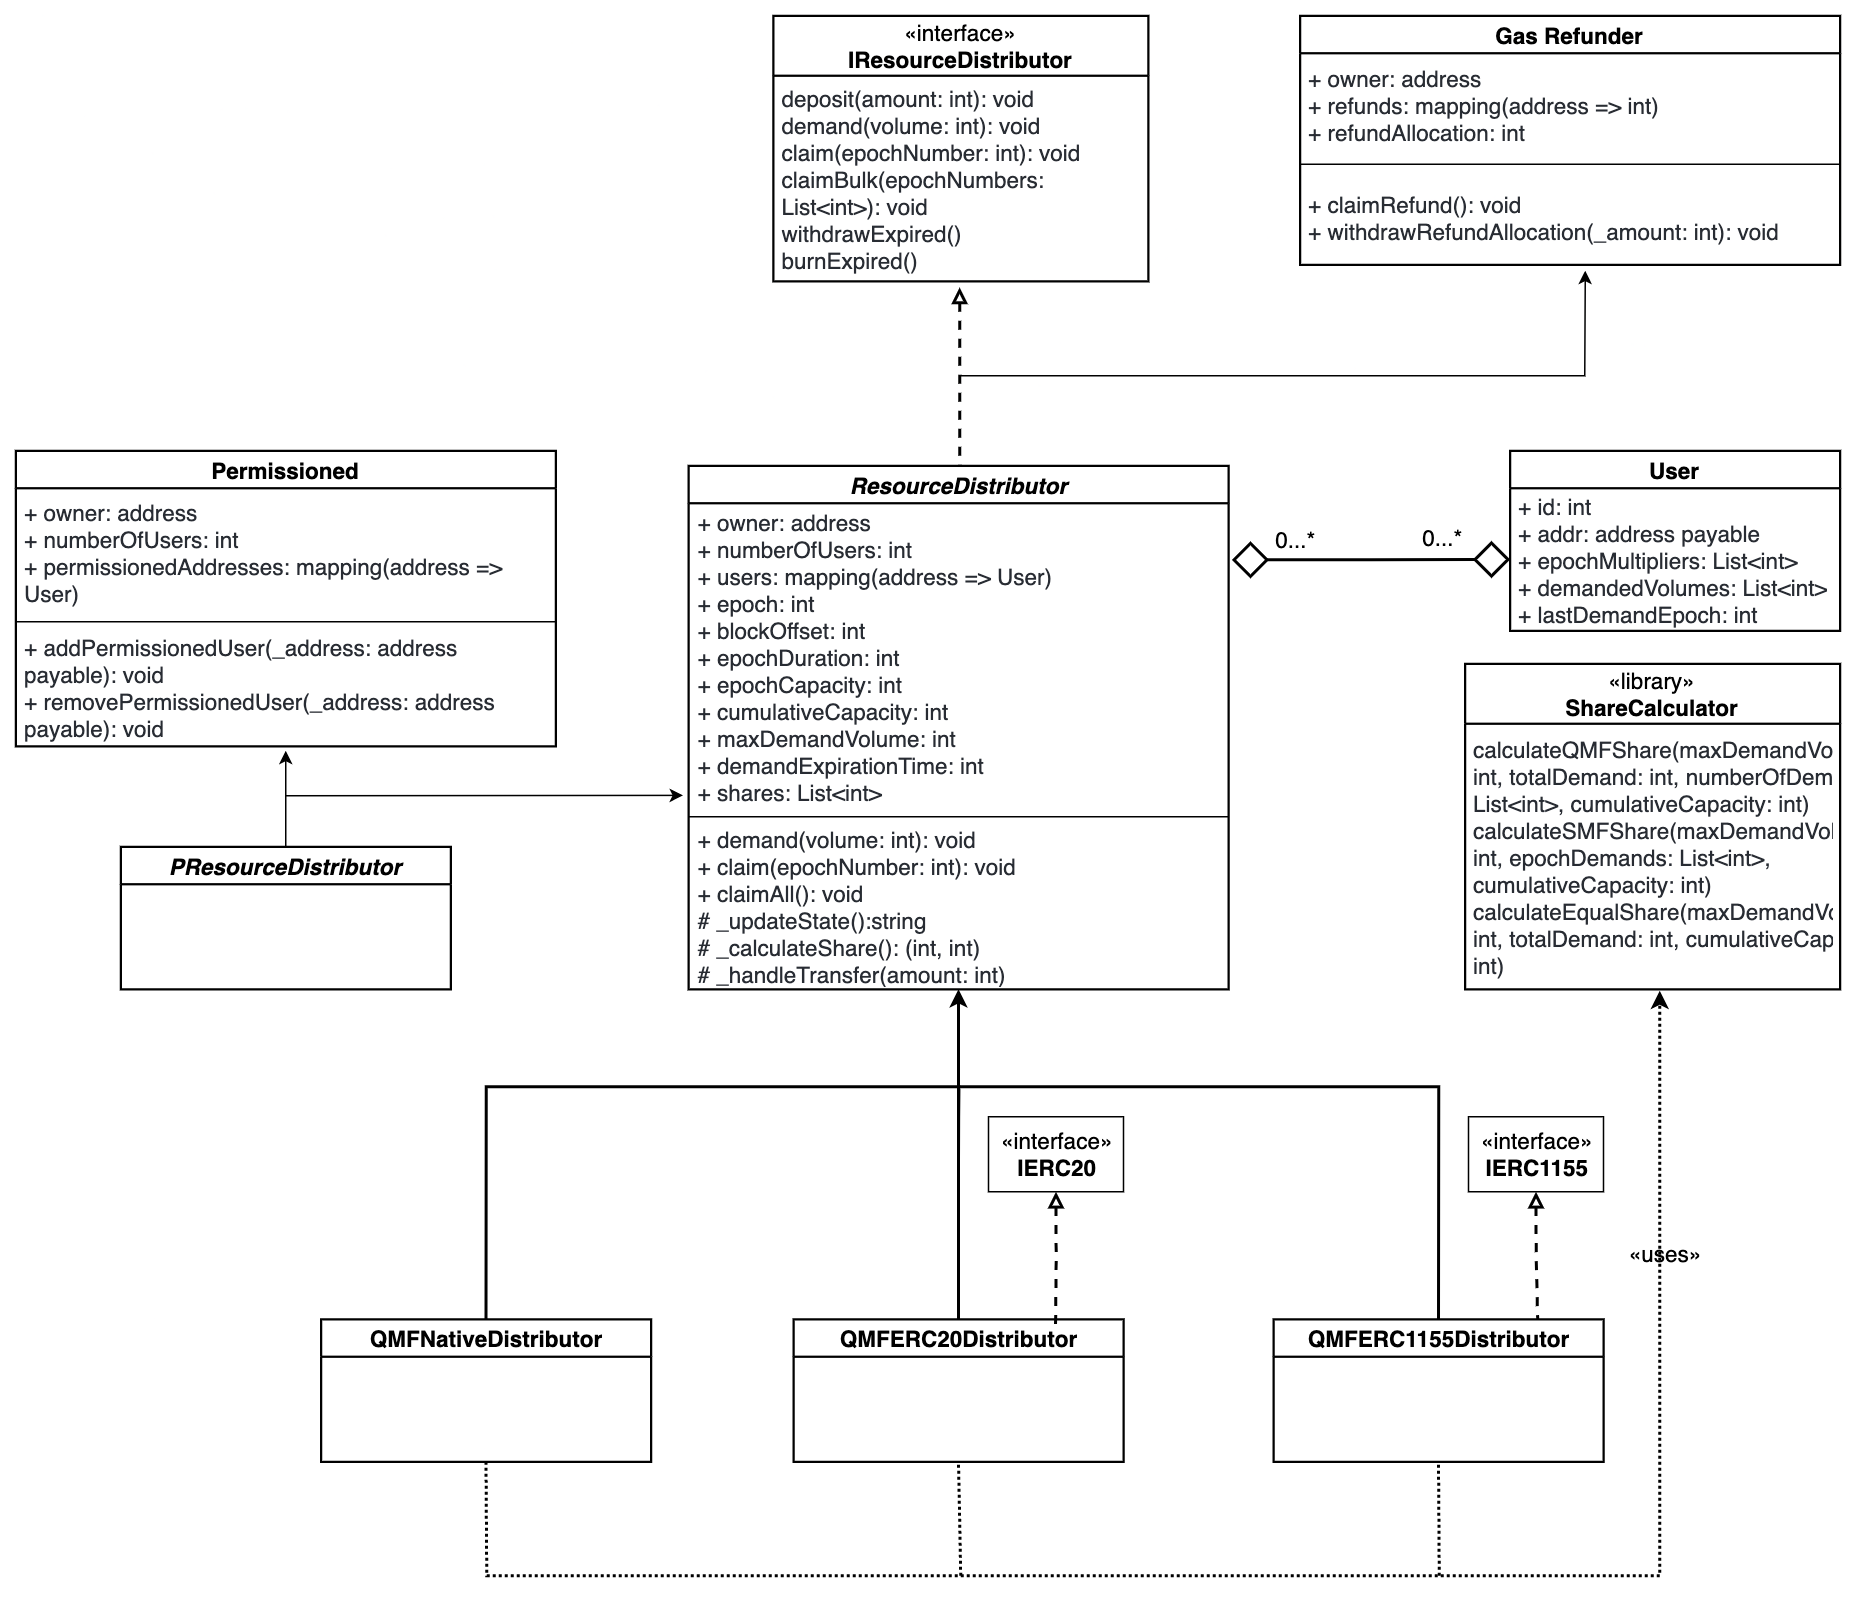
\includegraphics[width=0.9\textwidth]{class2.png}
	\caption{UML Class Diagram for Contracts}
\end{figure}

\section{User Interface Design}
\subsection{Home Page}
\begin{figure}[H]
	\centering
	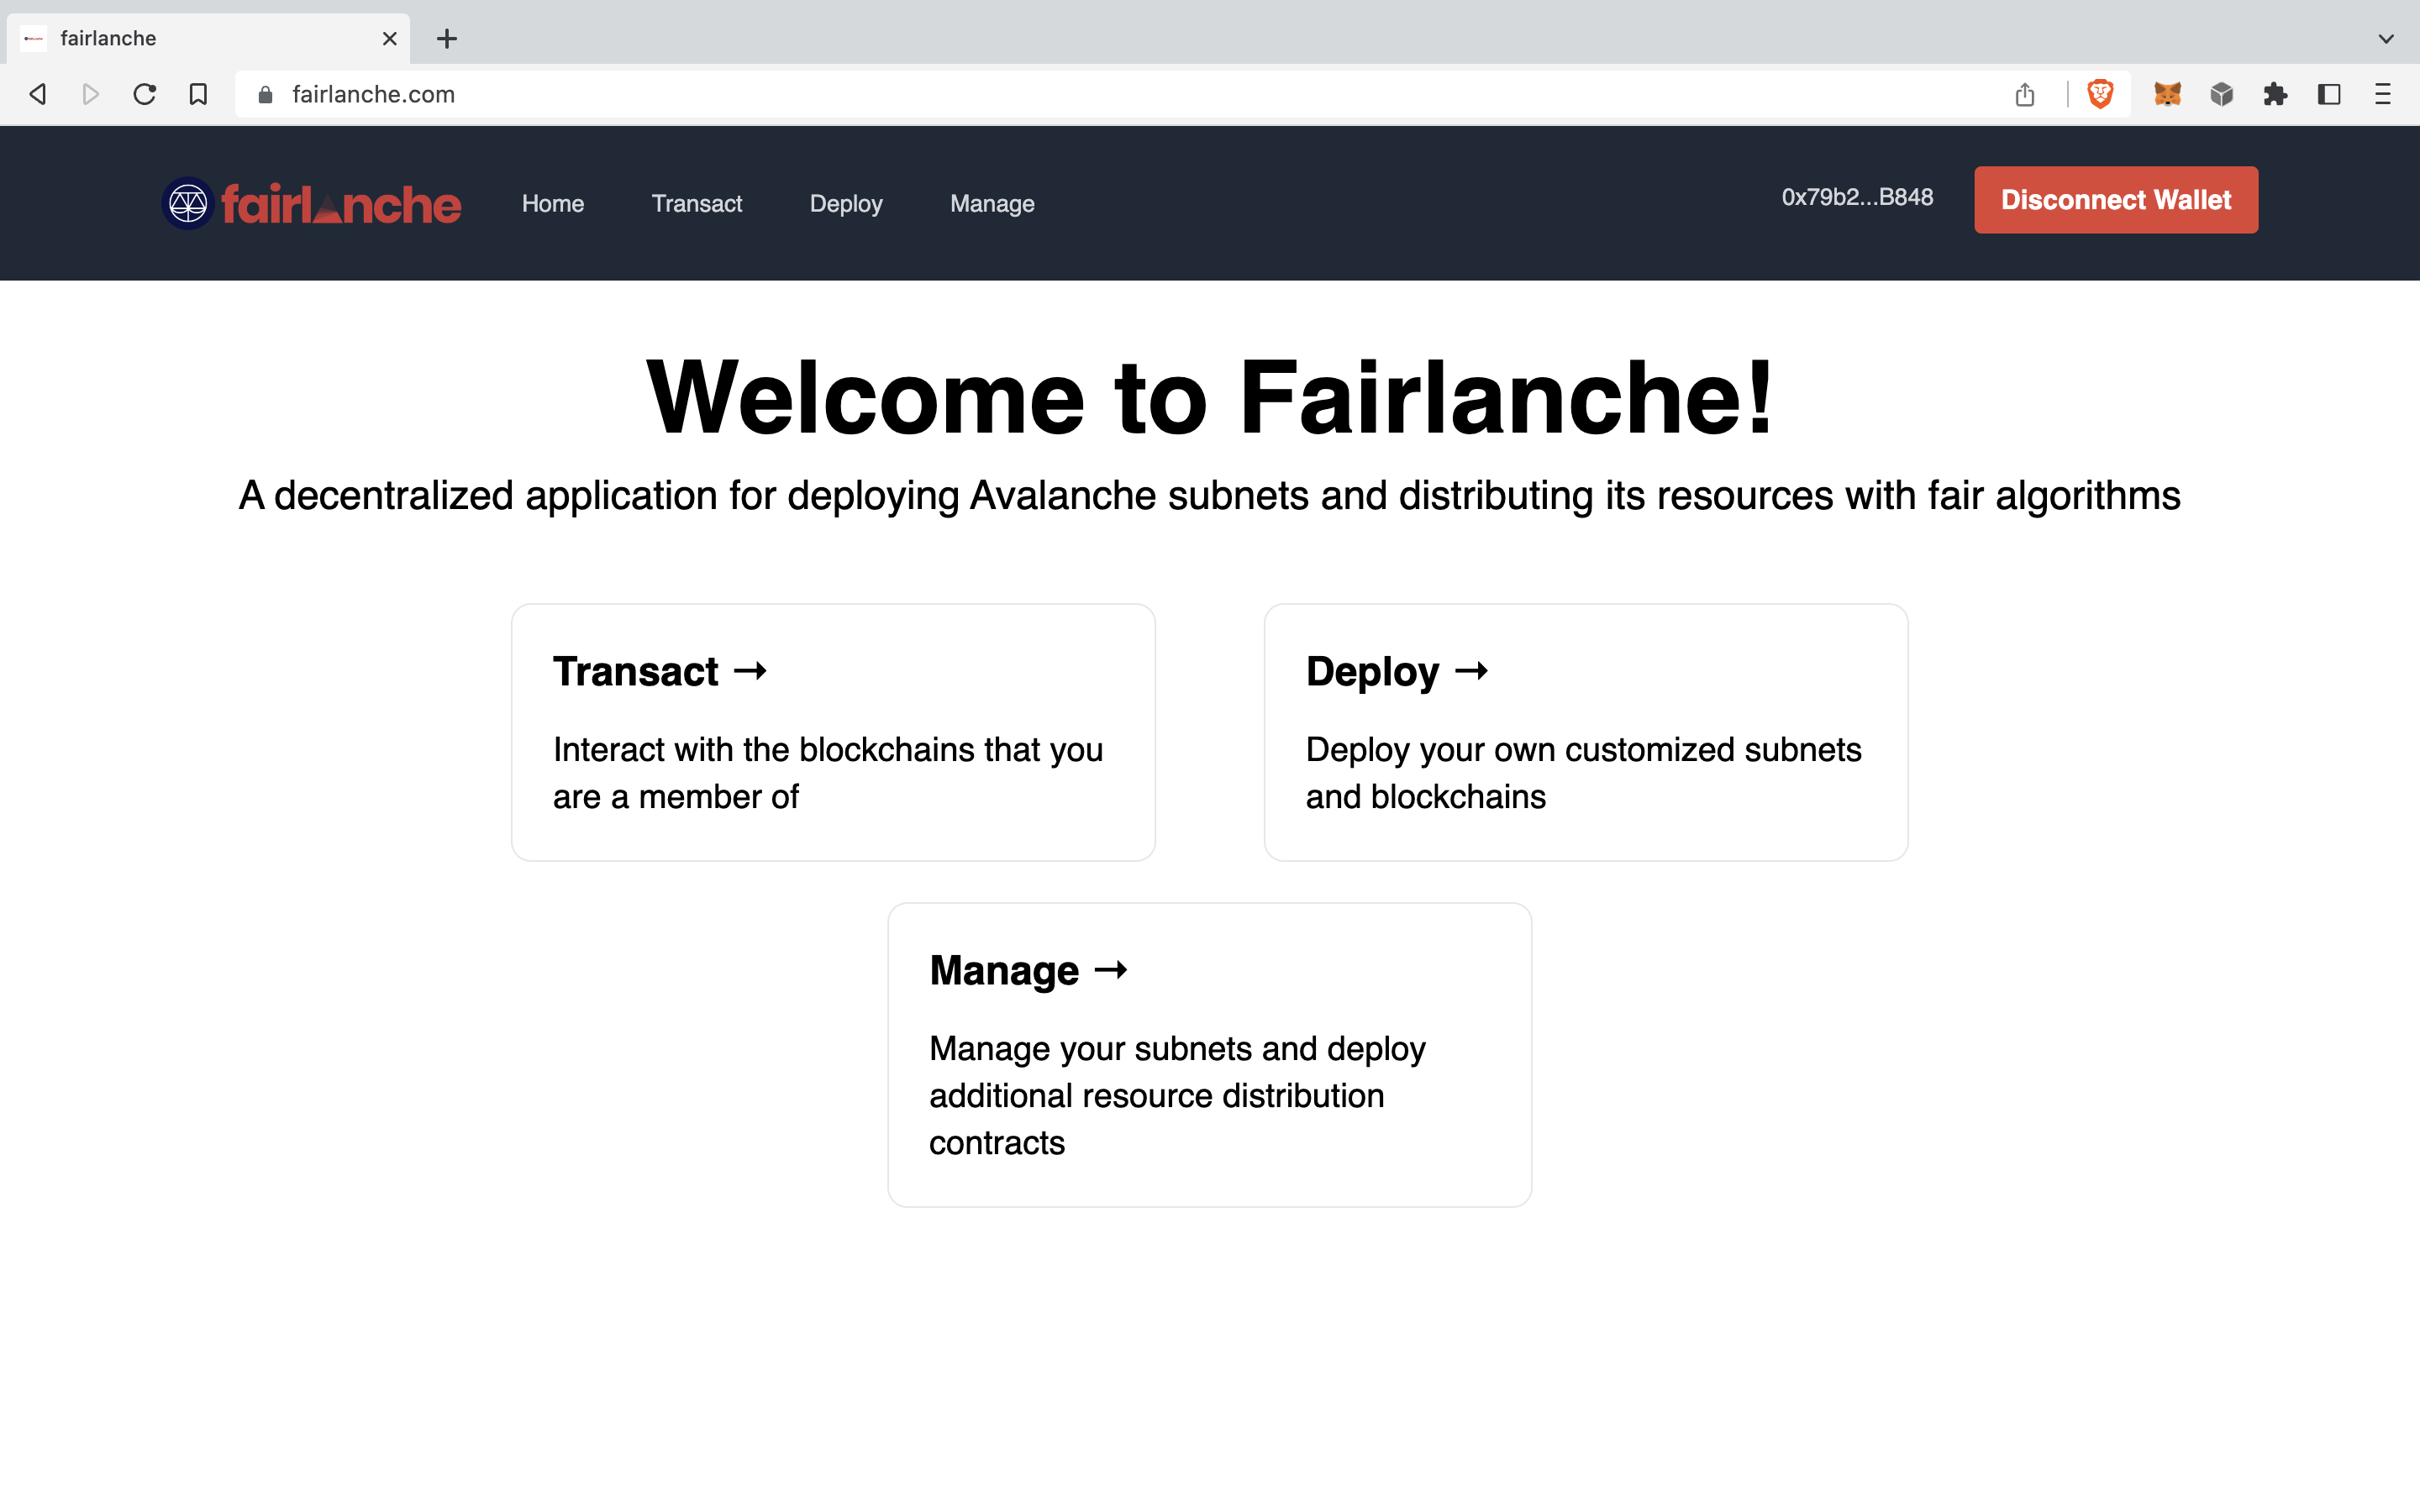
\includegraphics[width=1\textwidth]{ss1.png}
	\caption{Homepage UI}
\end{figure}
\subsection{Deployment Page}
\begin{figure}[H]
	\centering
	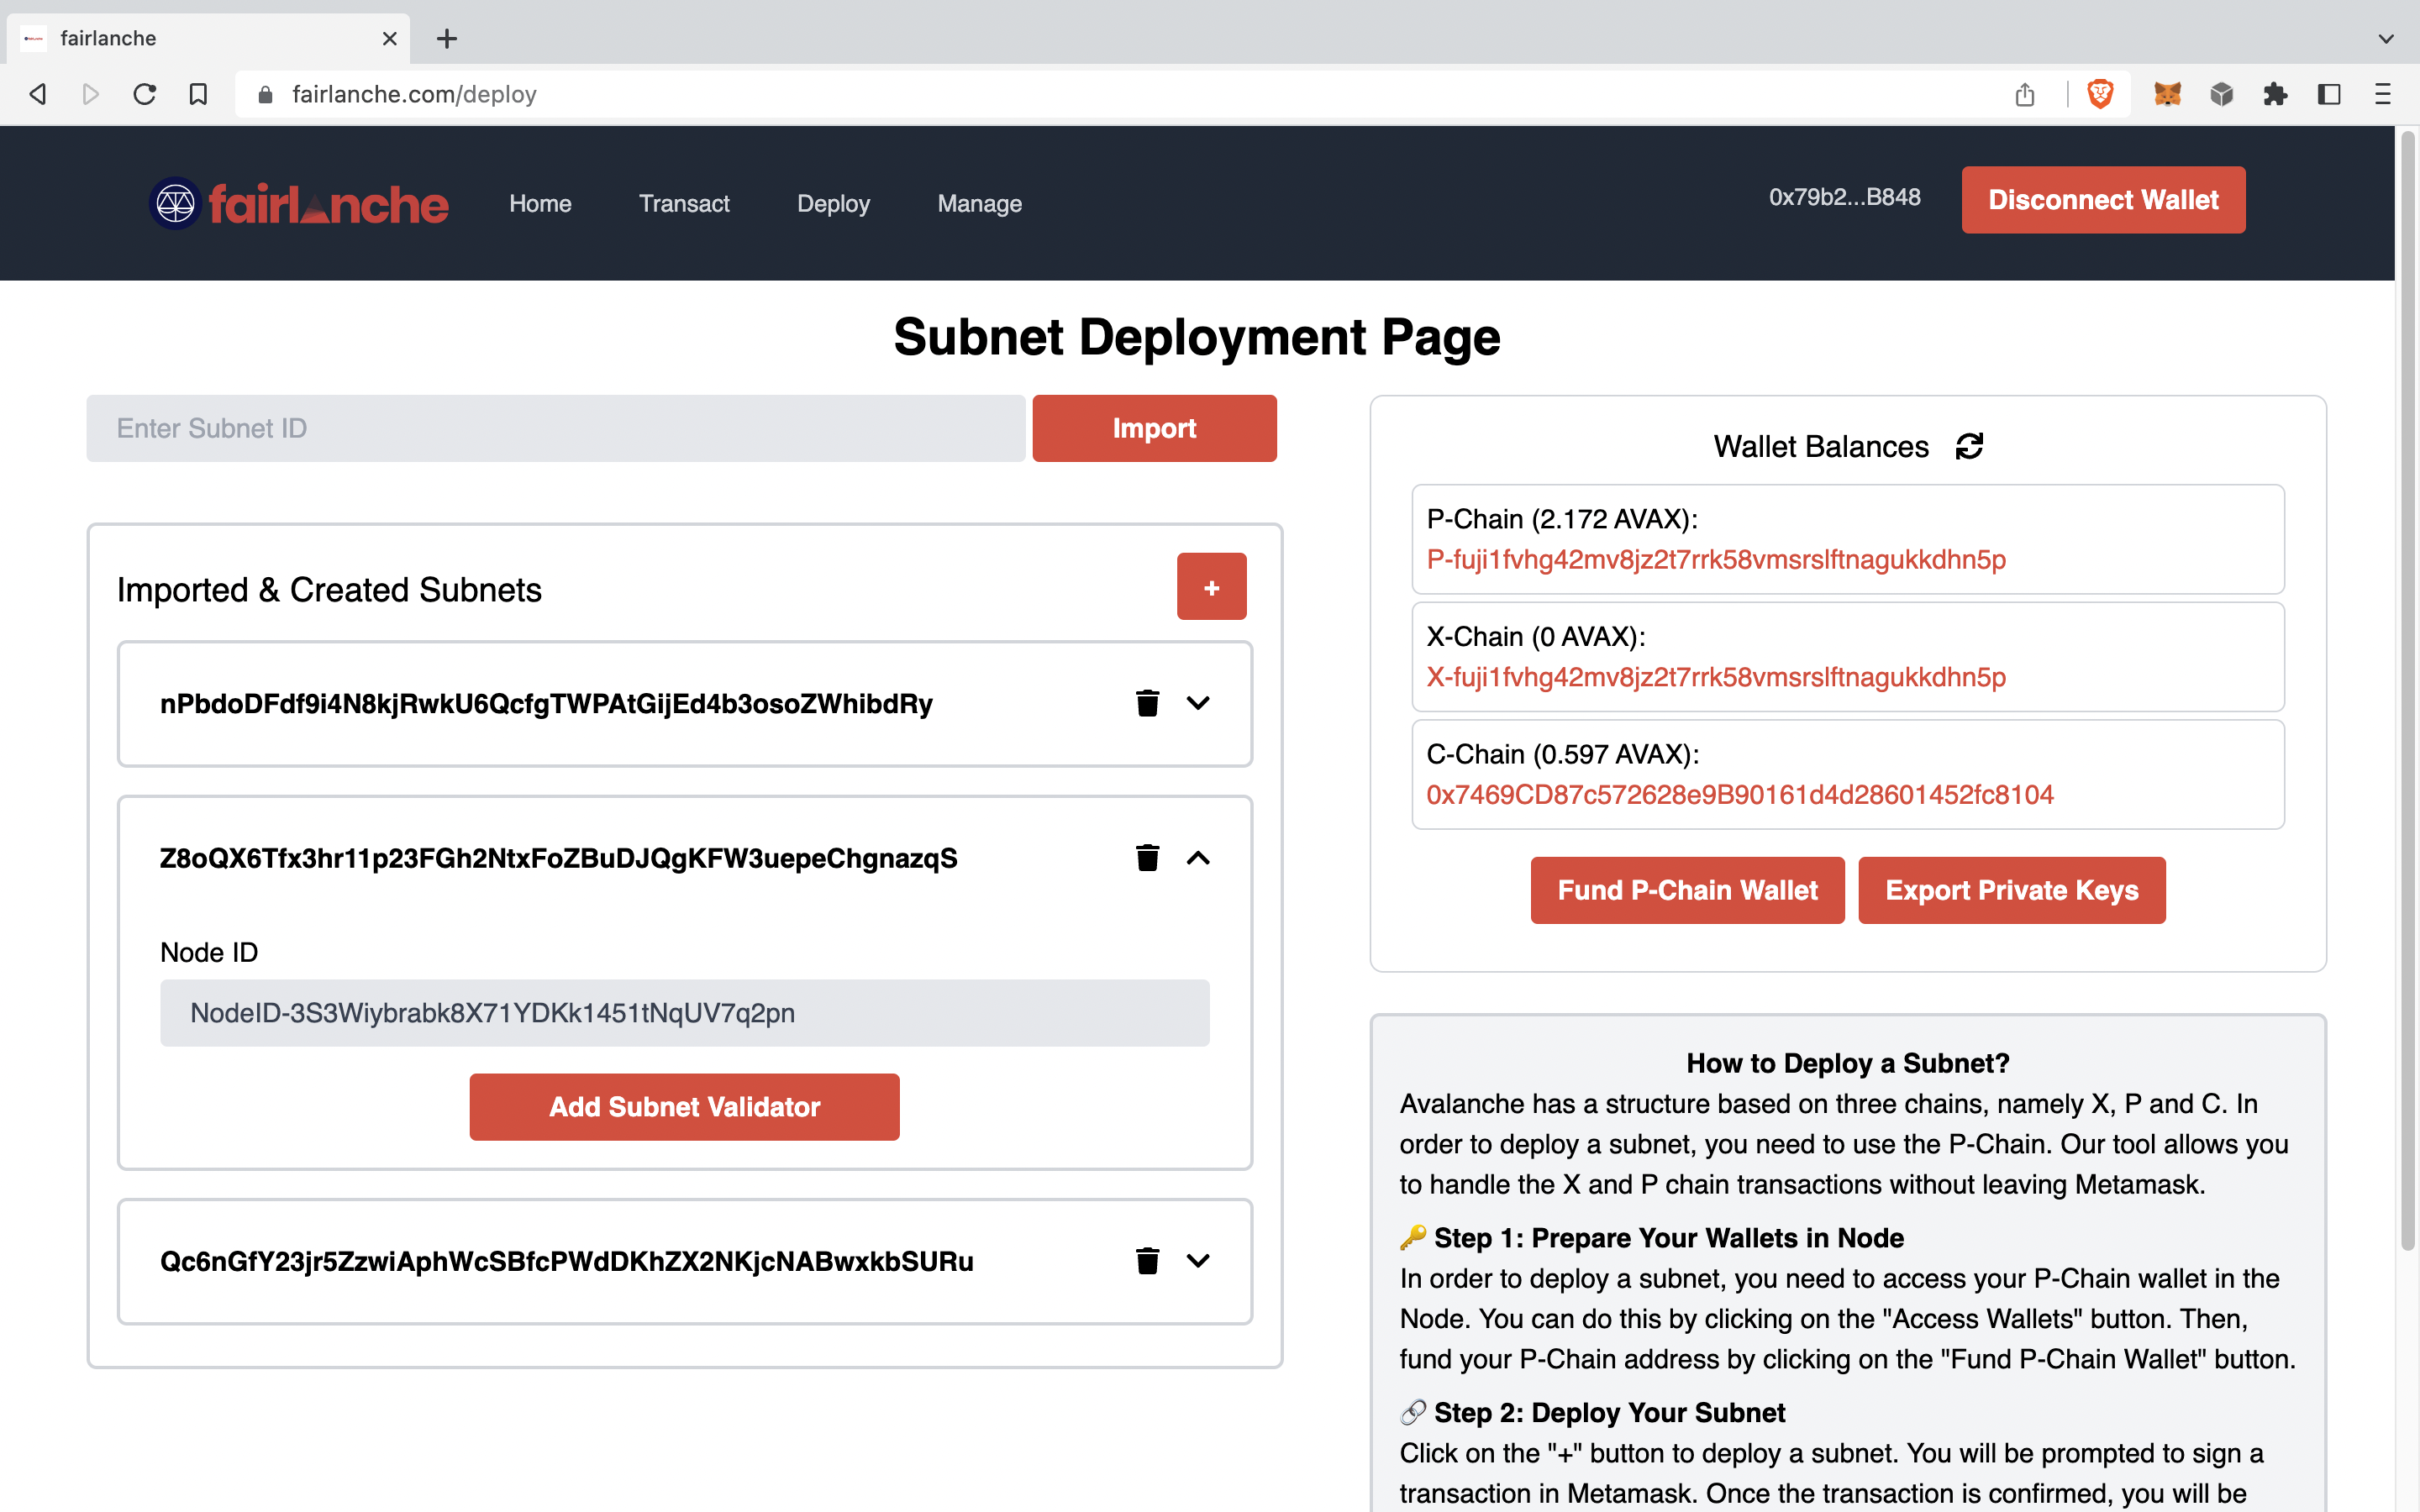
\includegraphics[width=1\textwidth]{ss2.png}
	\caption{Subnet Deployment Page UI}
\end{figure}
\begin{figure}[H]
	\centering
	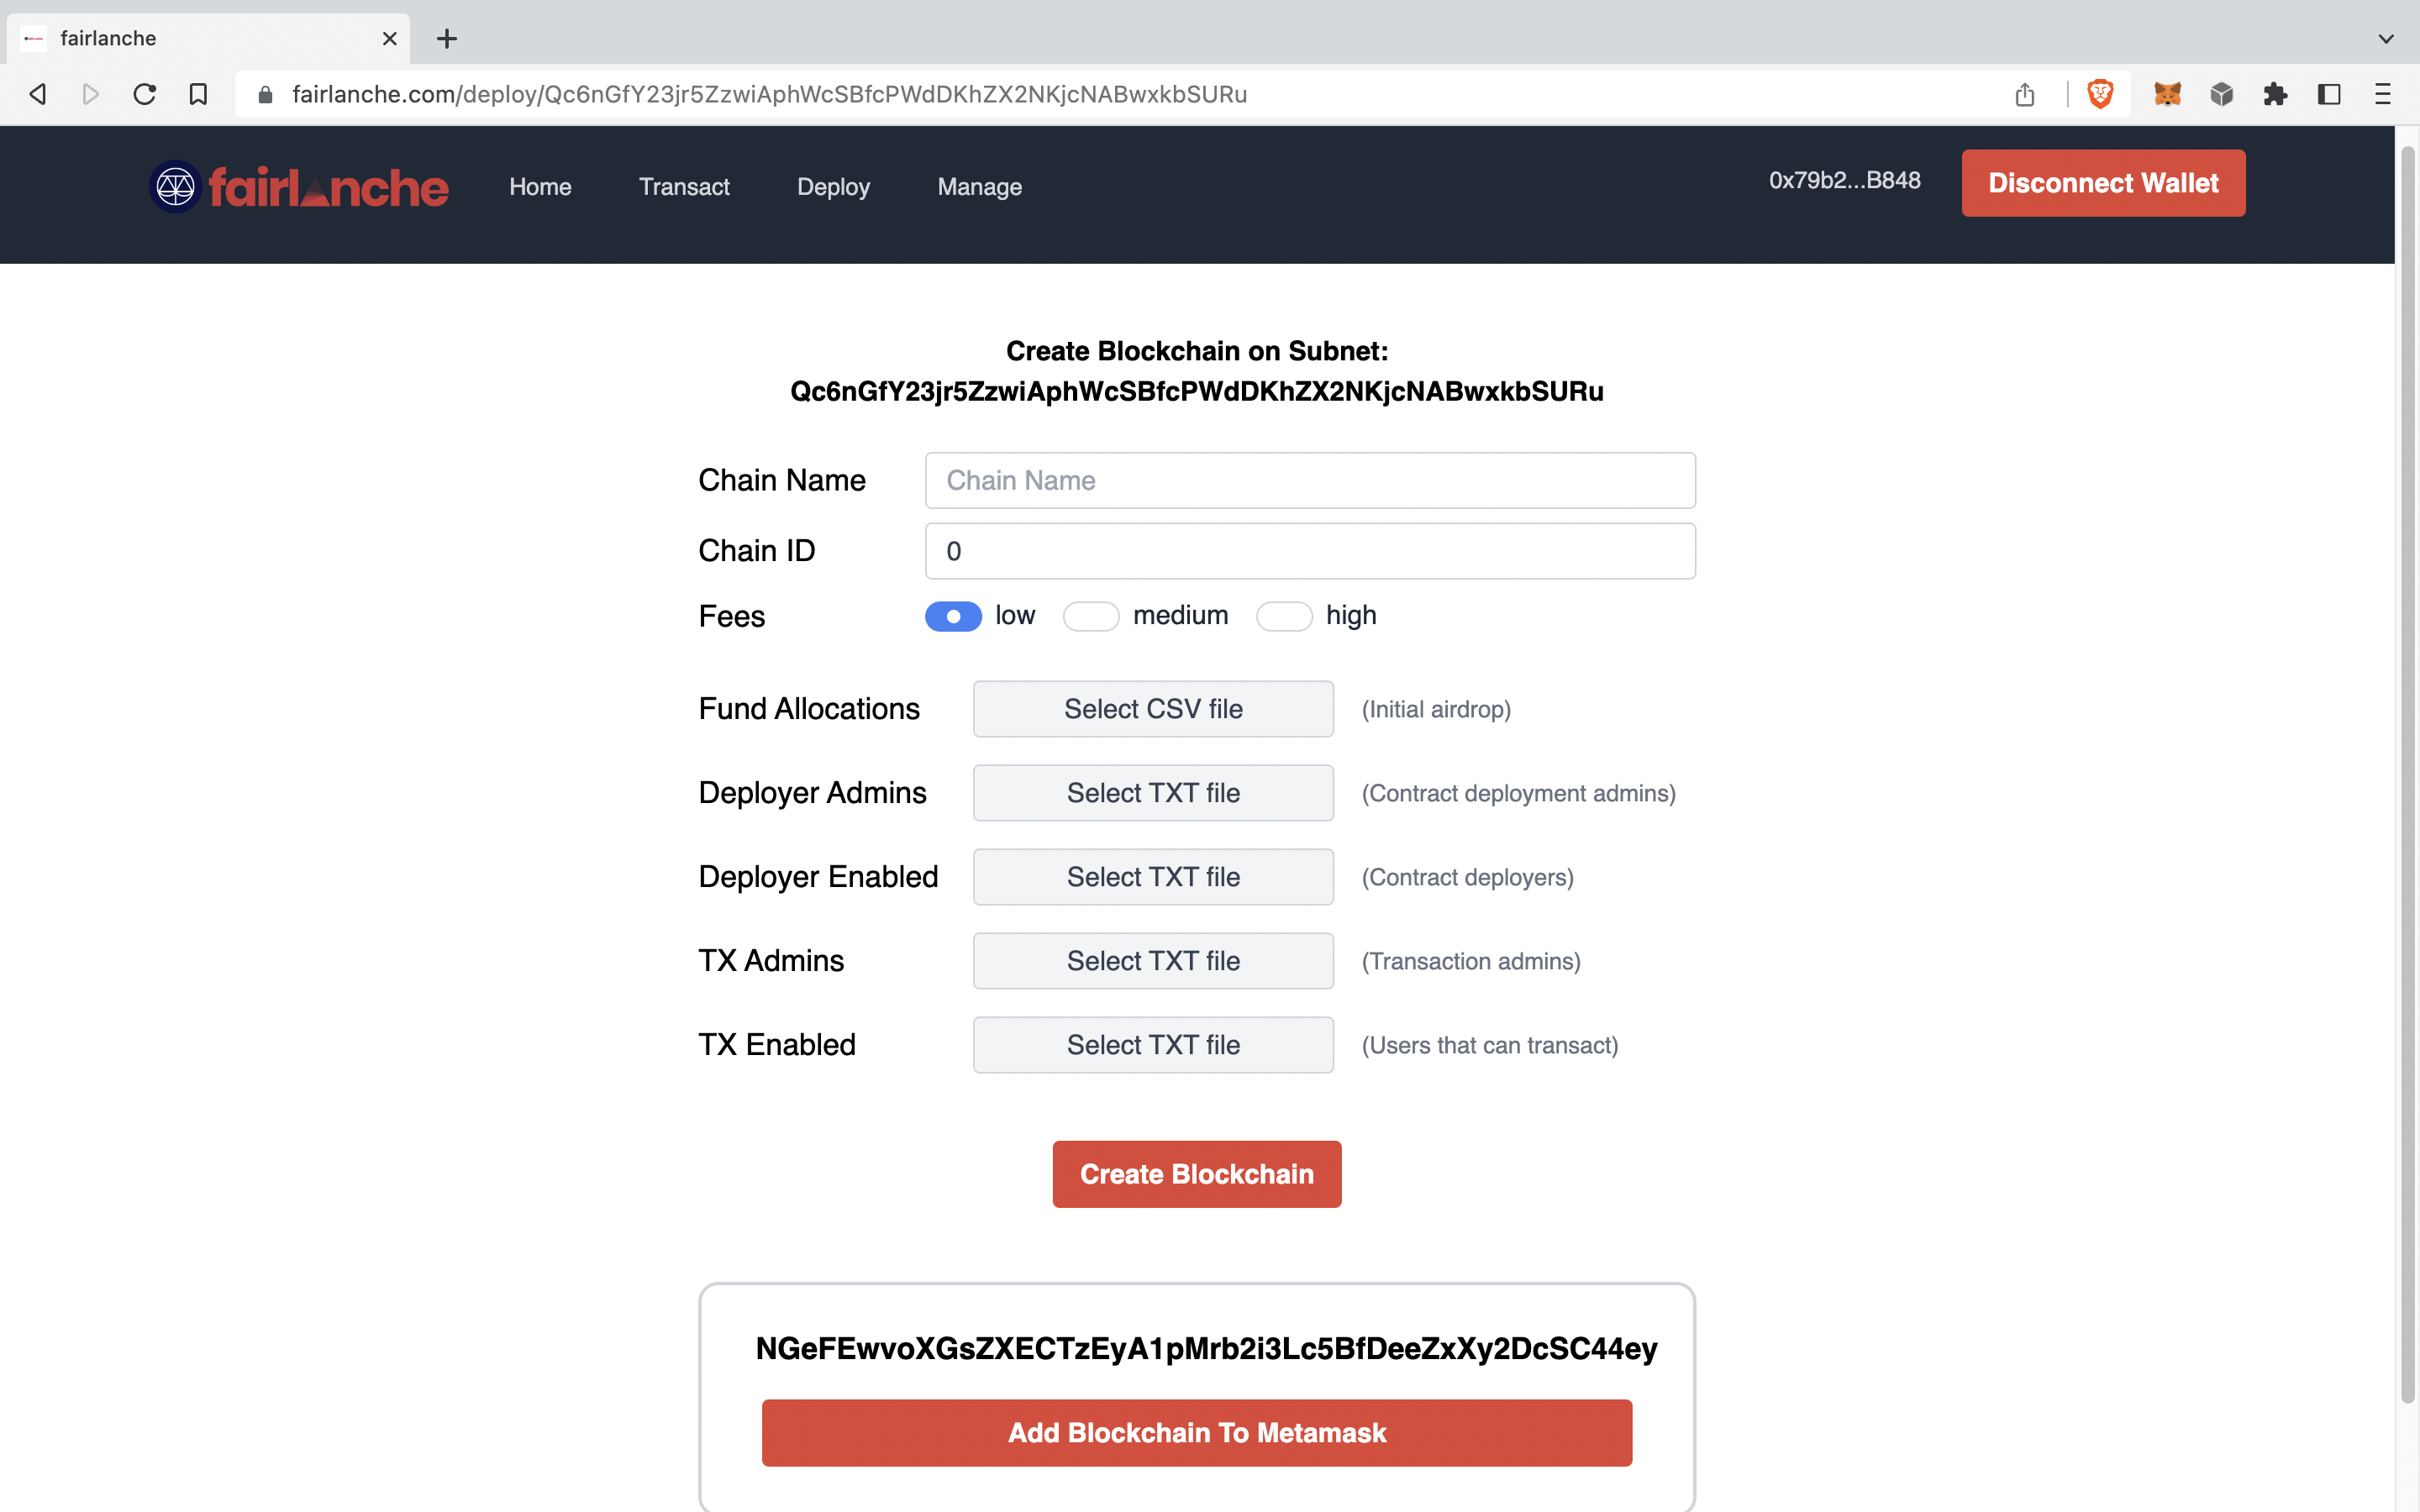
\includegraphics[width=1\textwidth]{ss3.png}
	\caption{Blockchain Creation Page UI}
\end{figure}
\subsection{Management Page}
\begin{figure}[H]
	\centering
	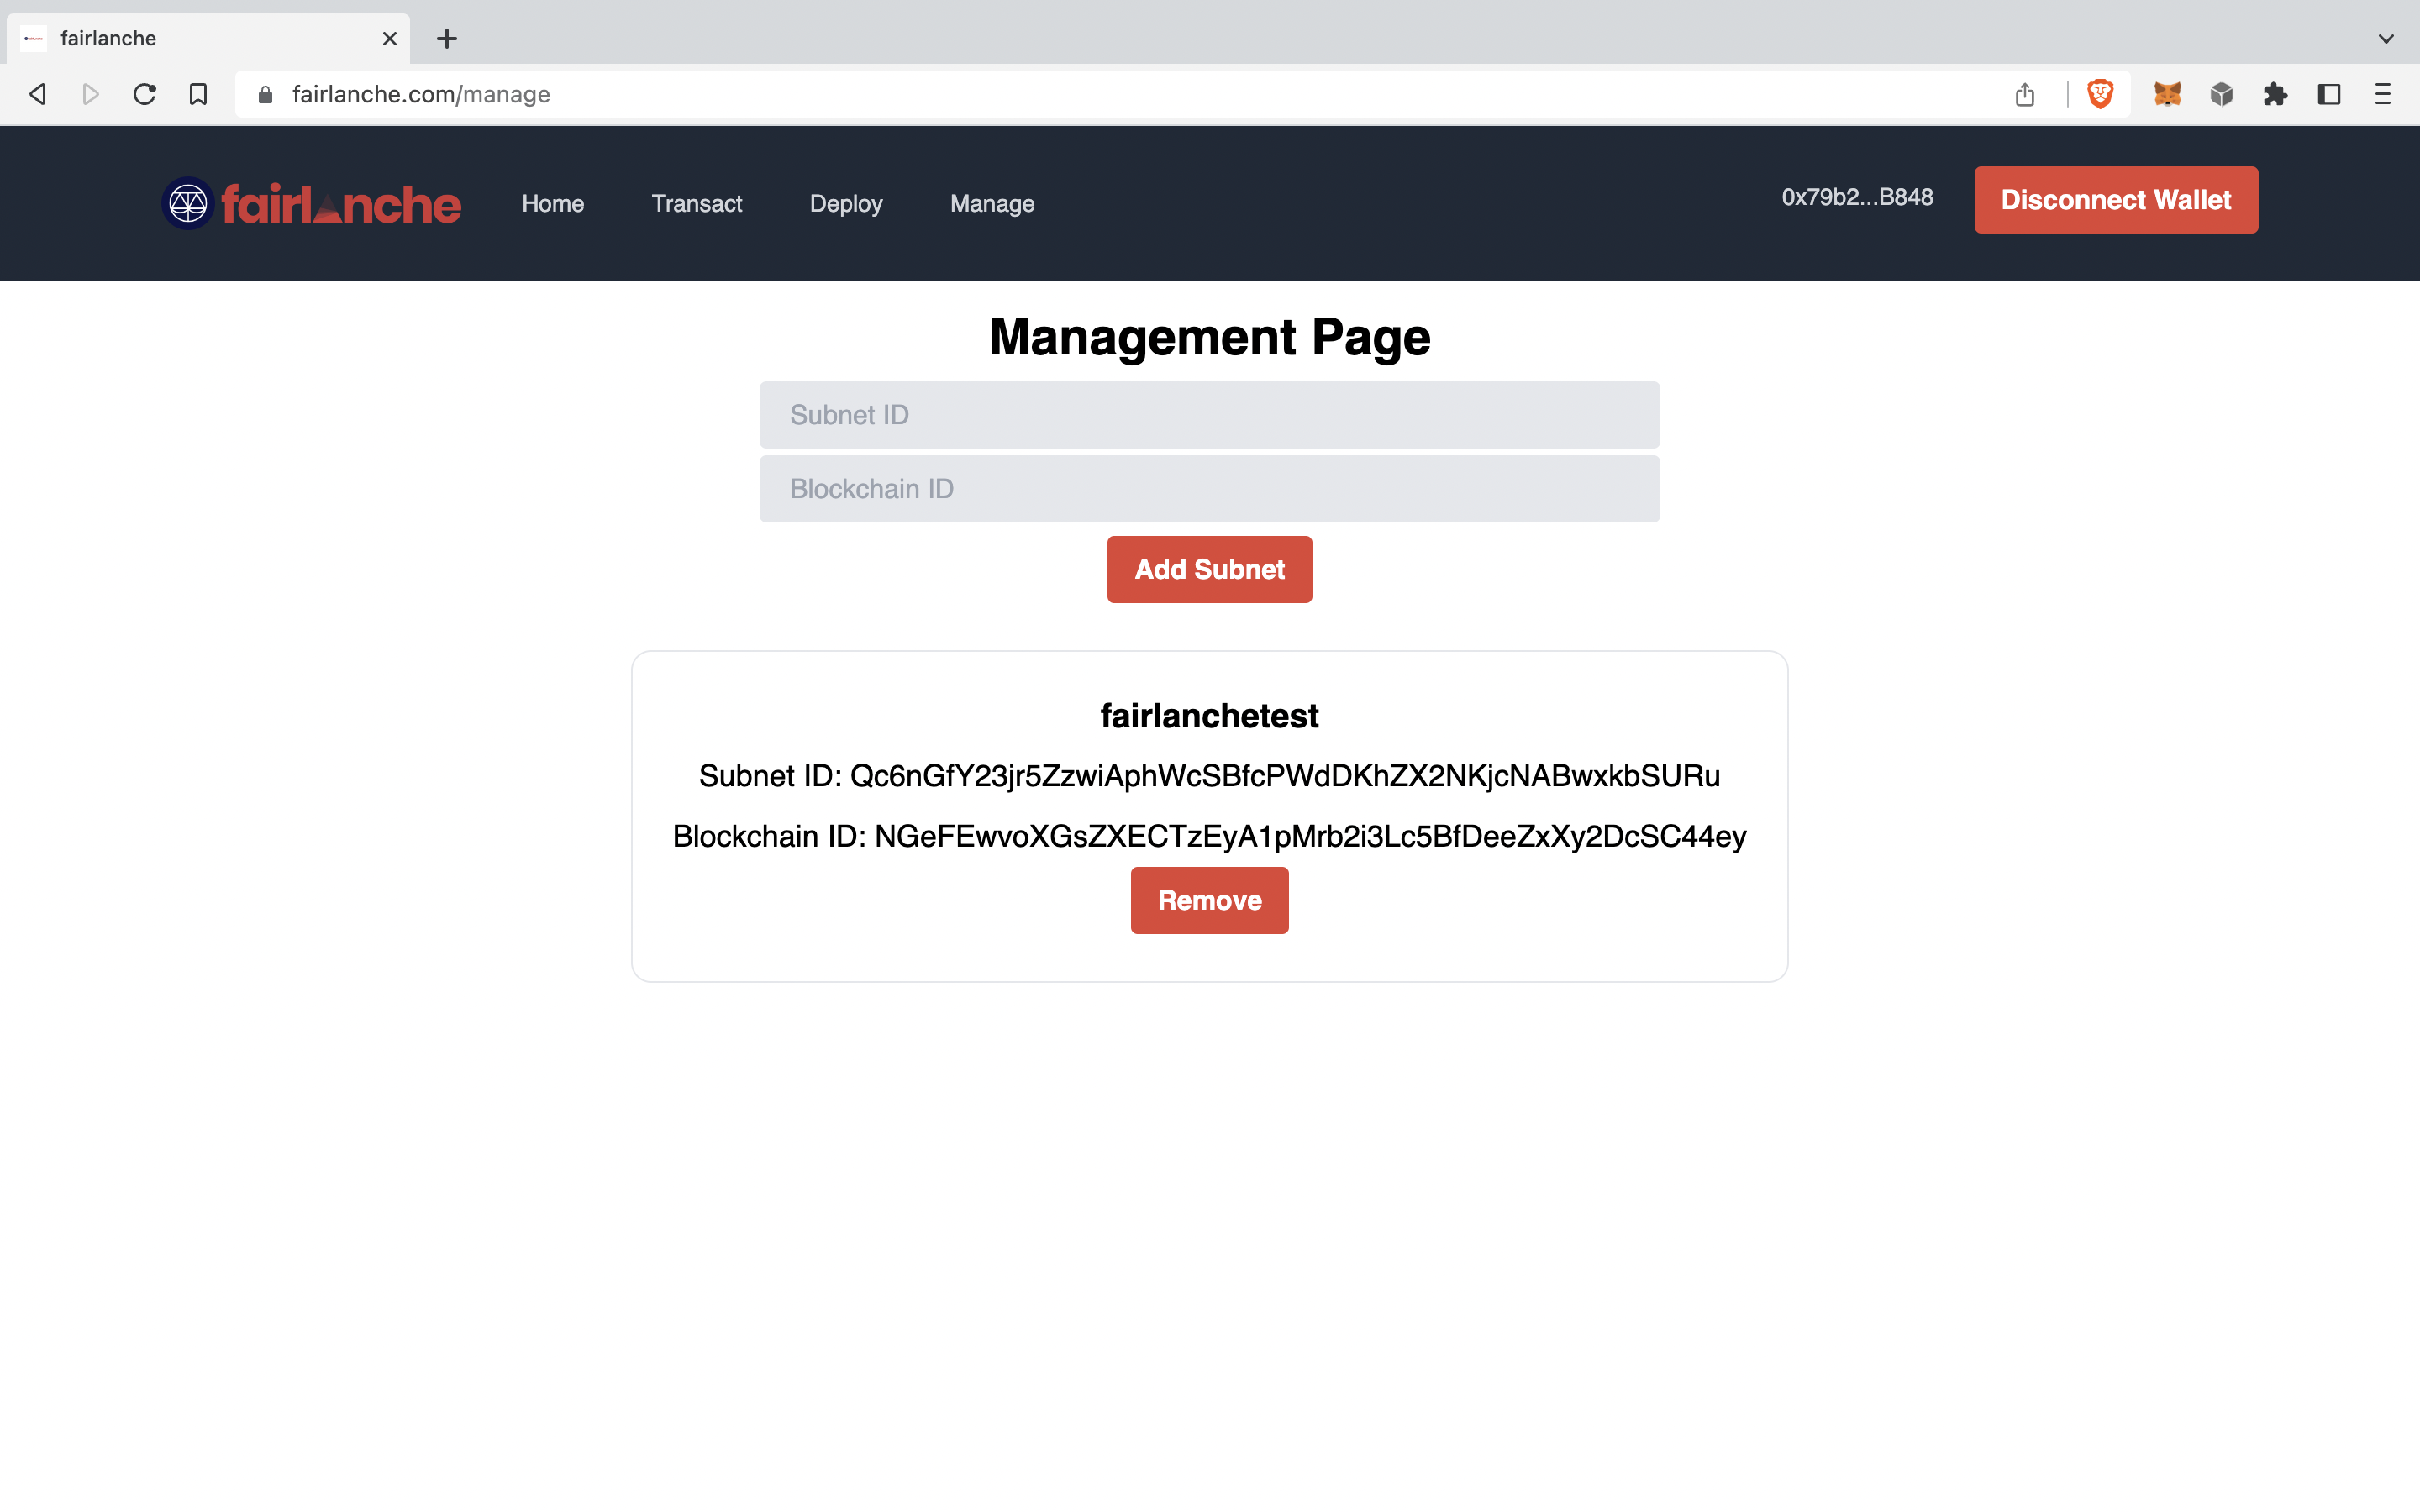
\includegraphics[width=1\textwidth]{ss4.png}
	\caption{Management Page UI}
\end{figure}
\begin{figure}[H]
	\centering
	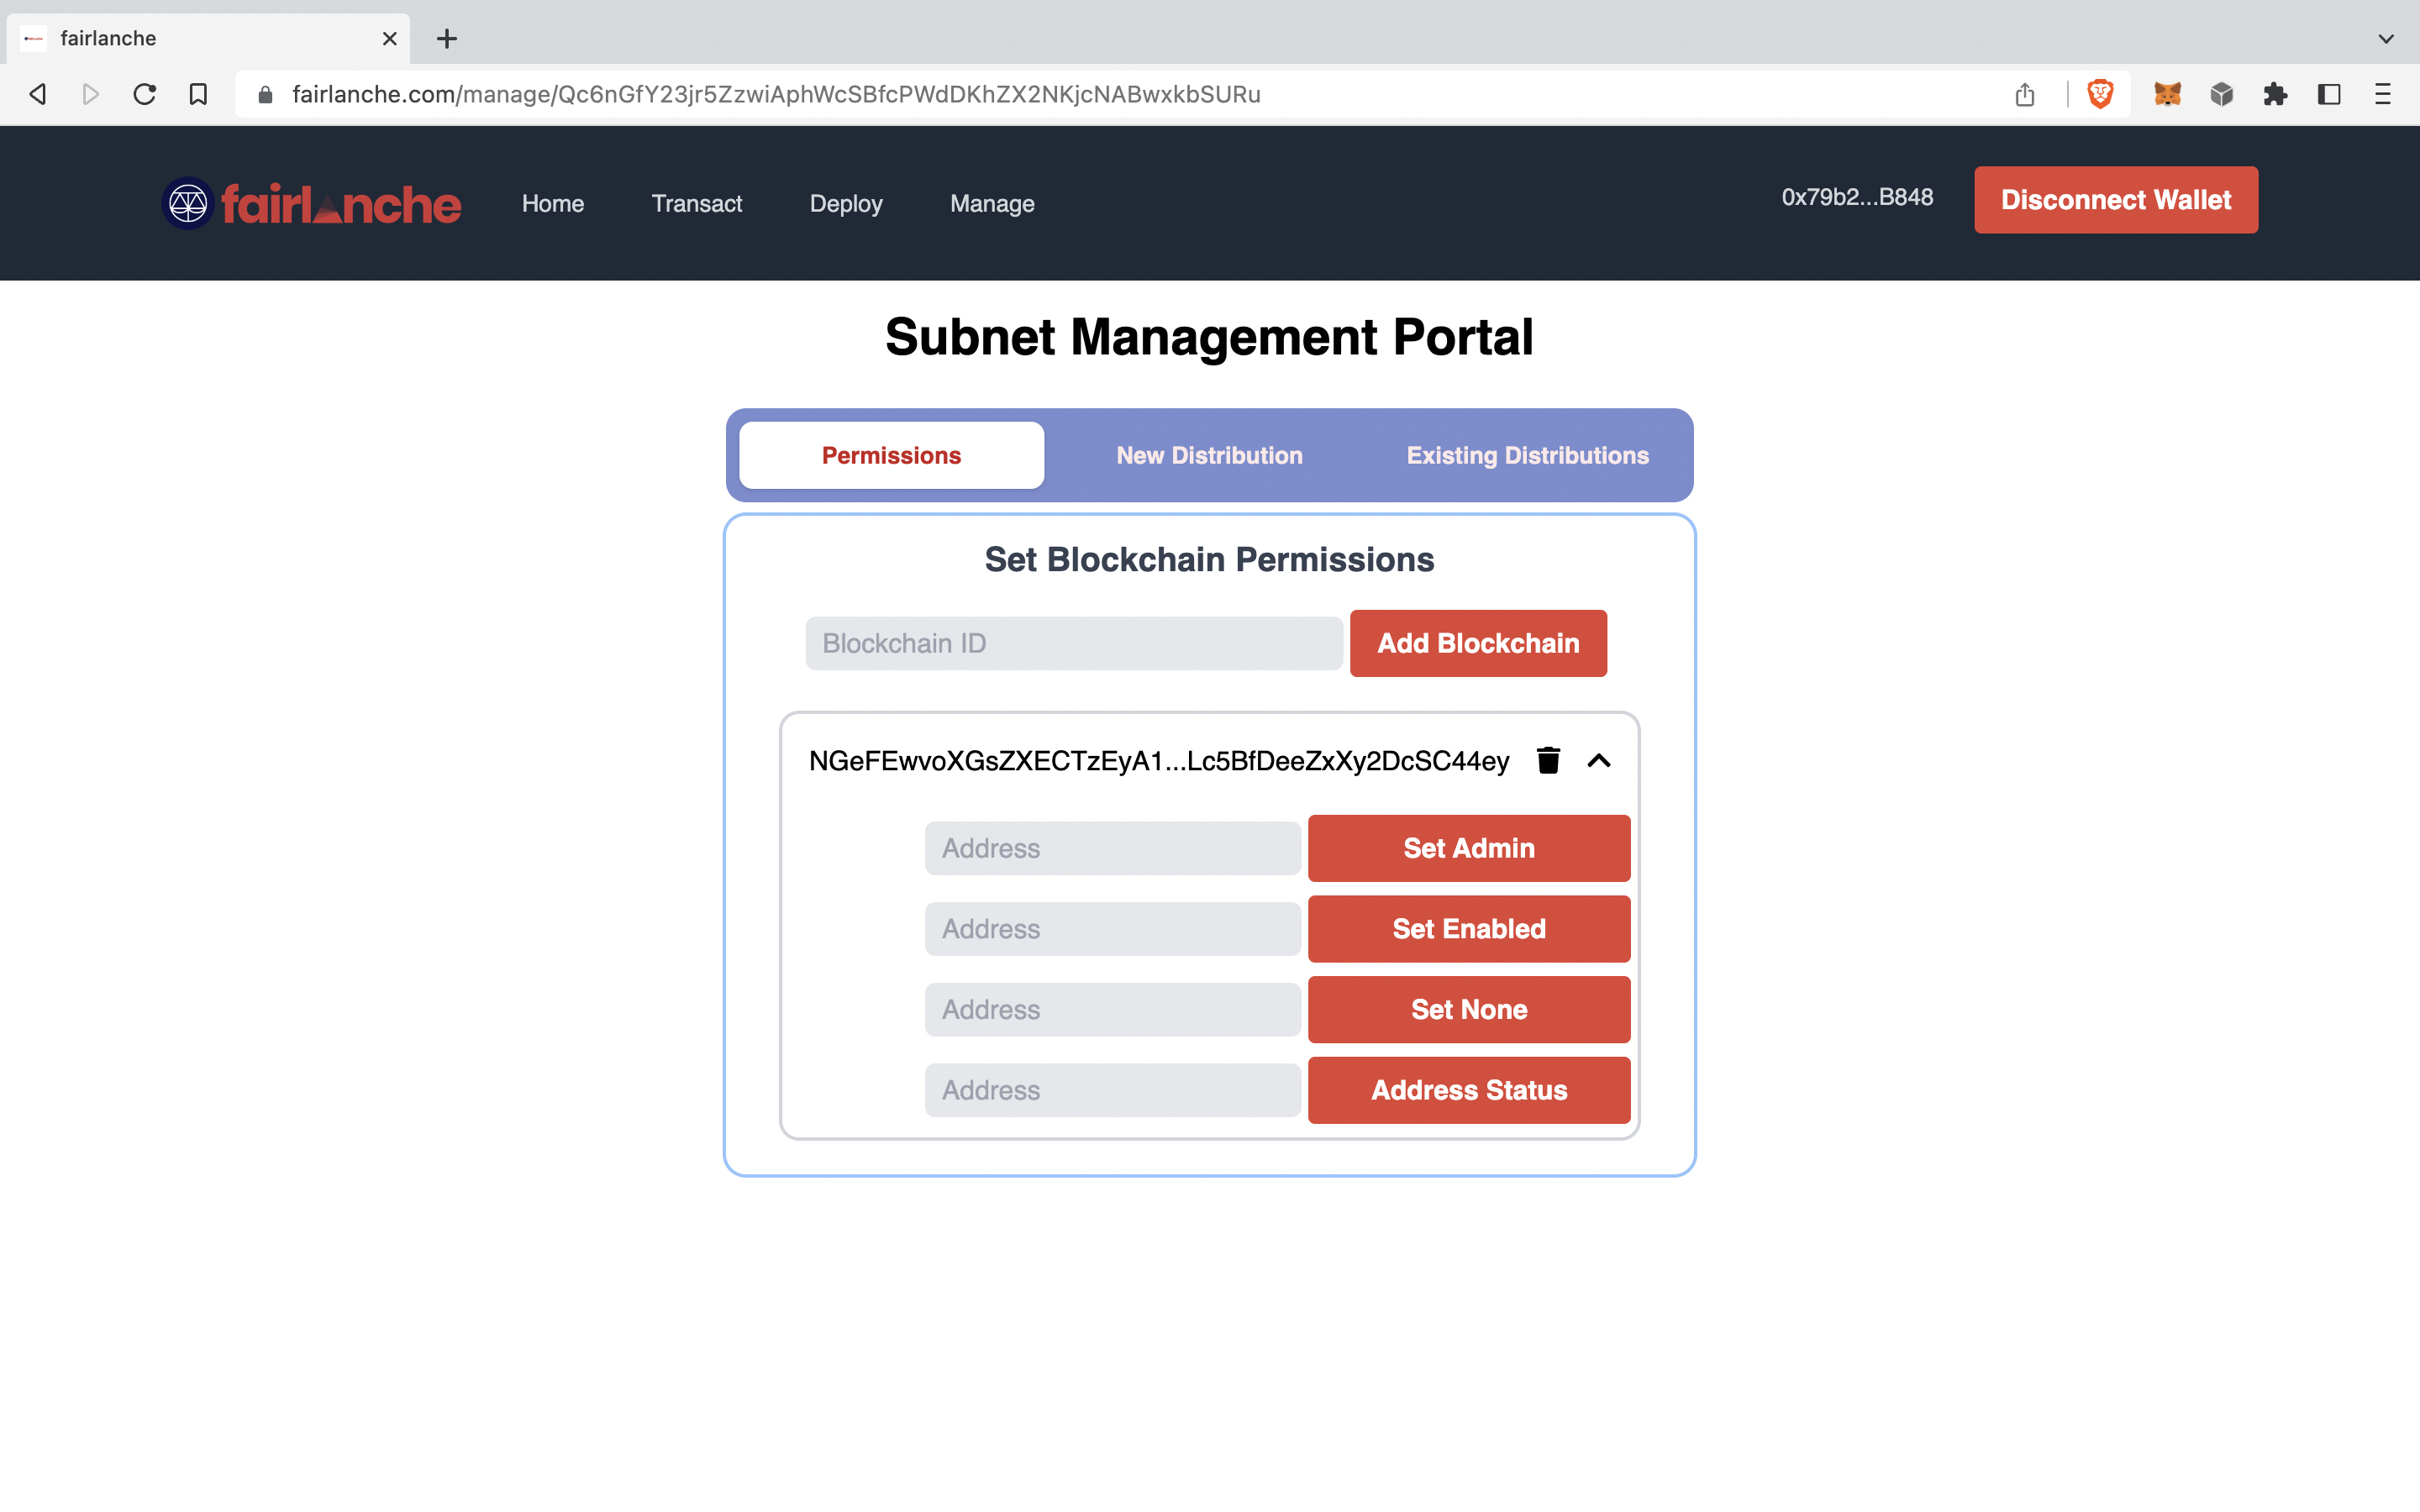
\includegraphics[width=1\textwidth]{ss5.png}
	\caption{Blockchain Permission Settings UI}
\end{figure}
\begin{figure}[H]
	\centering
	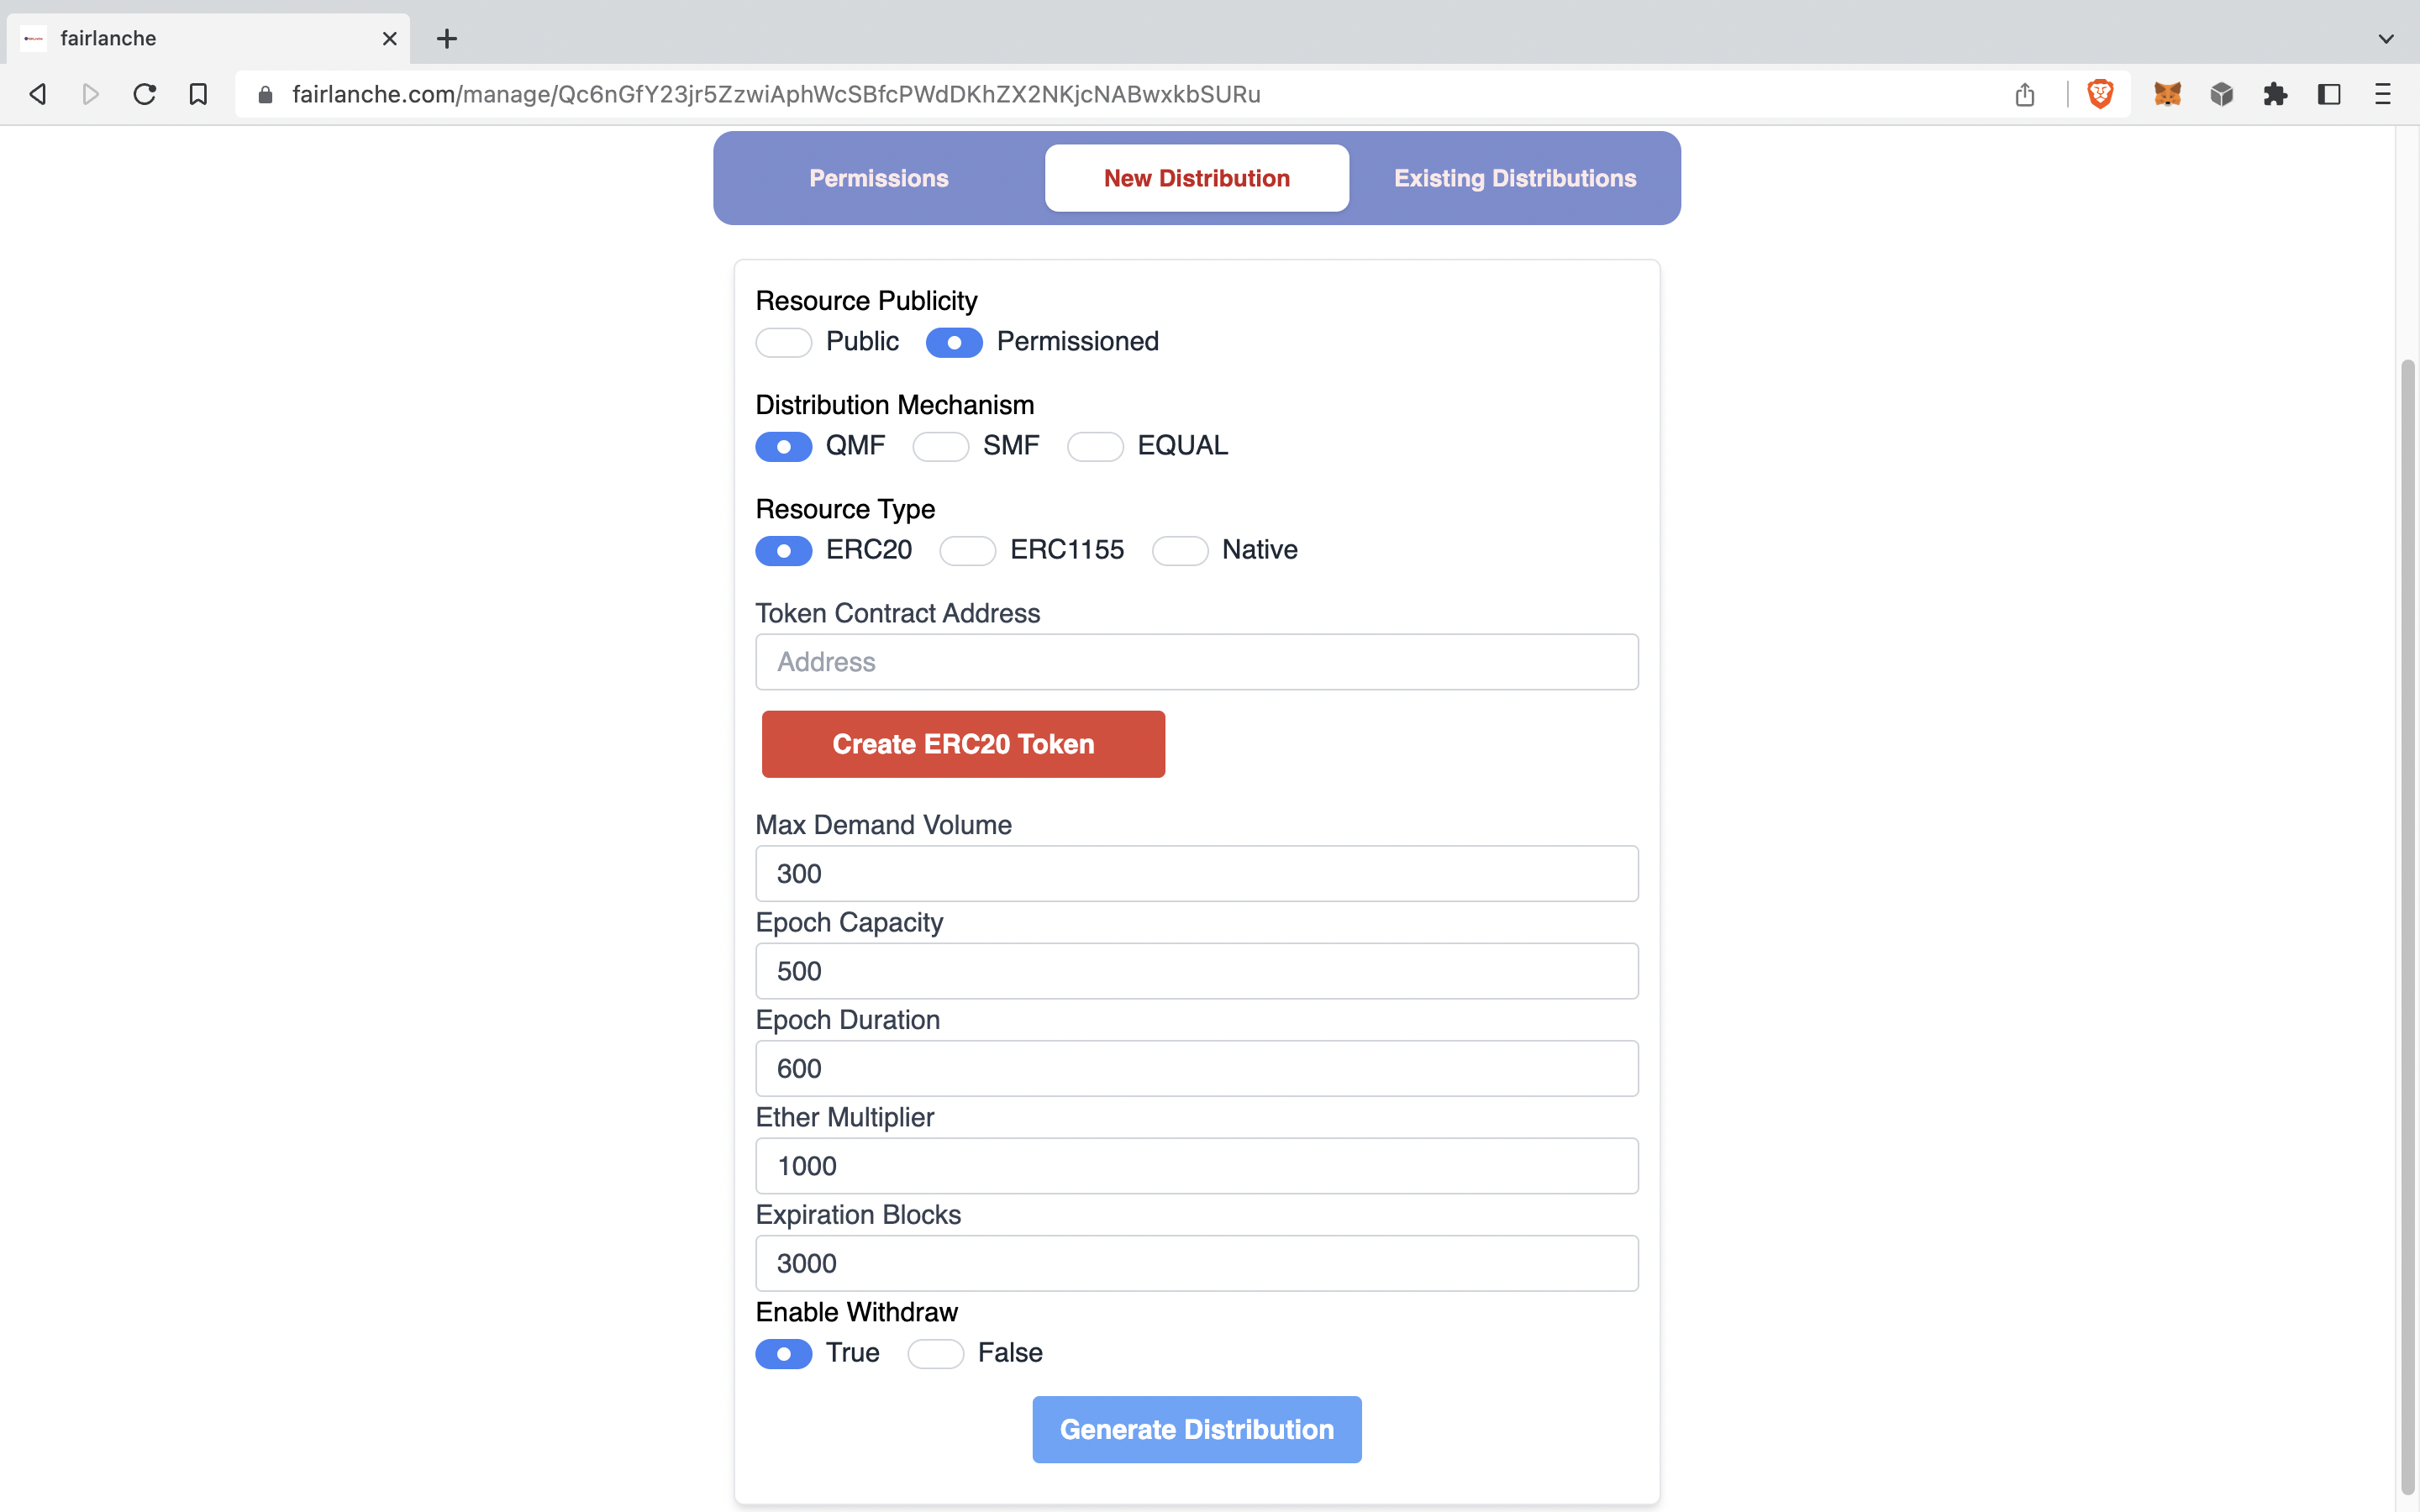
\includegraphics[width=1\textwidth]{ss6.png}
	\caption{Native Distributor Deploy UI}
\end{figure}
\begin{figure}[H]
	\centering
	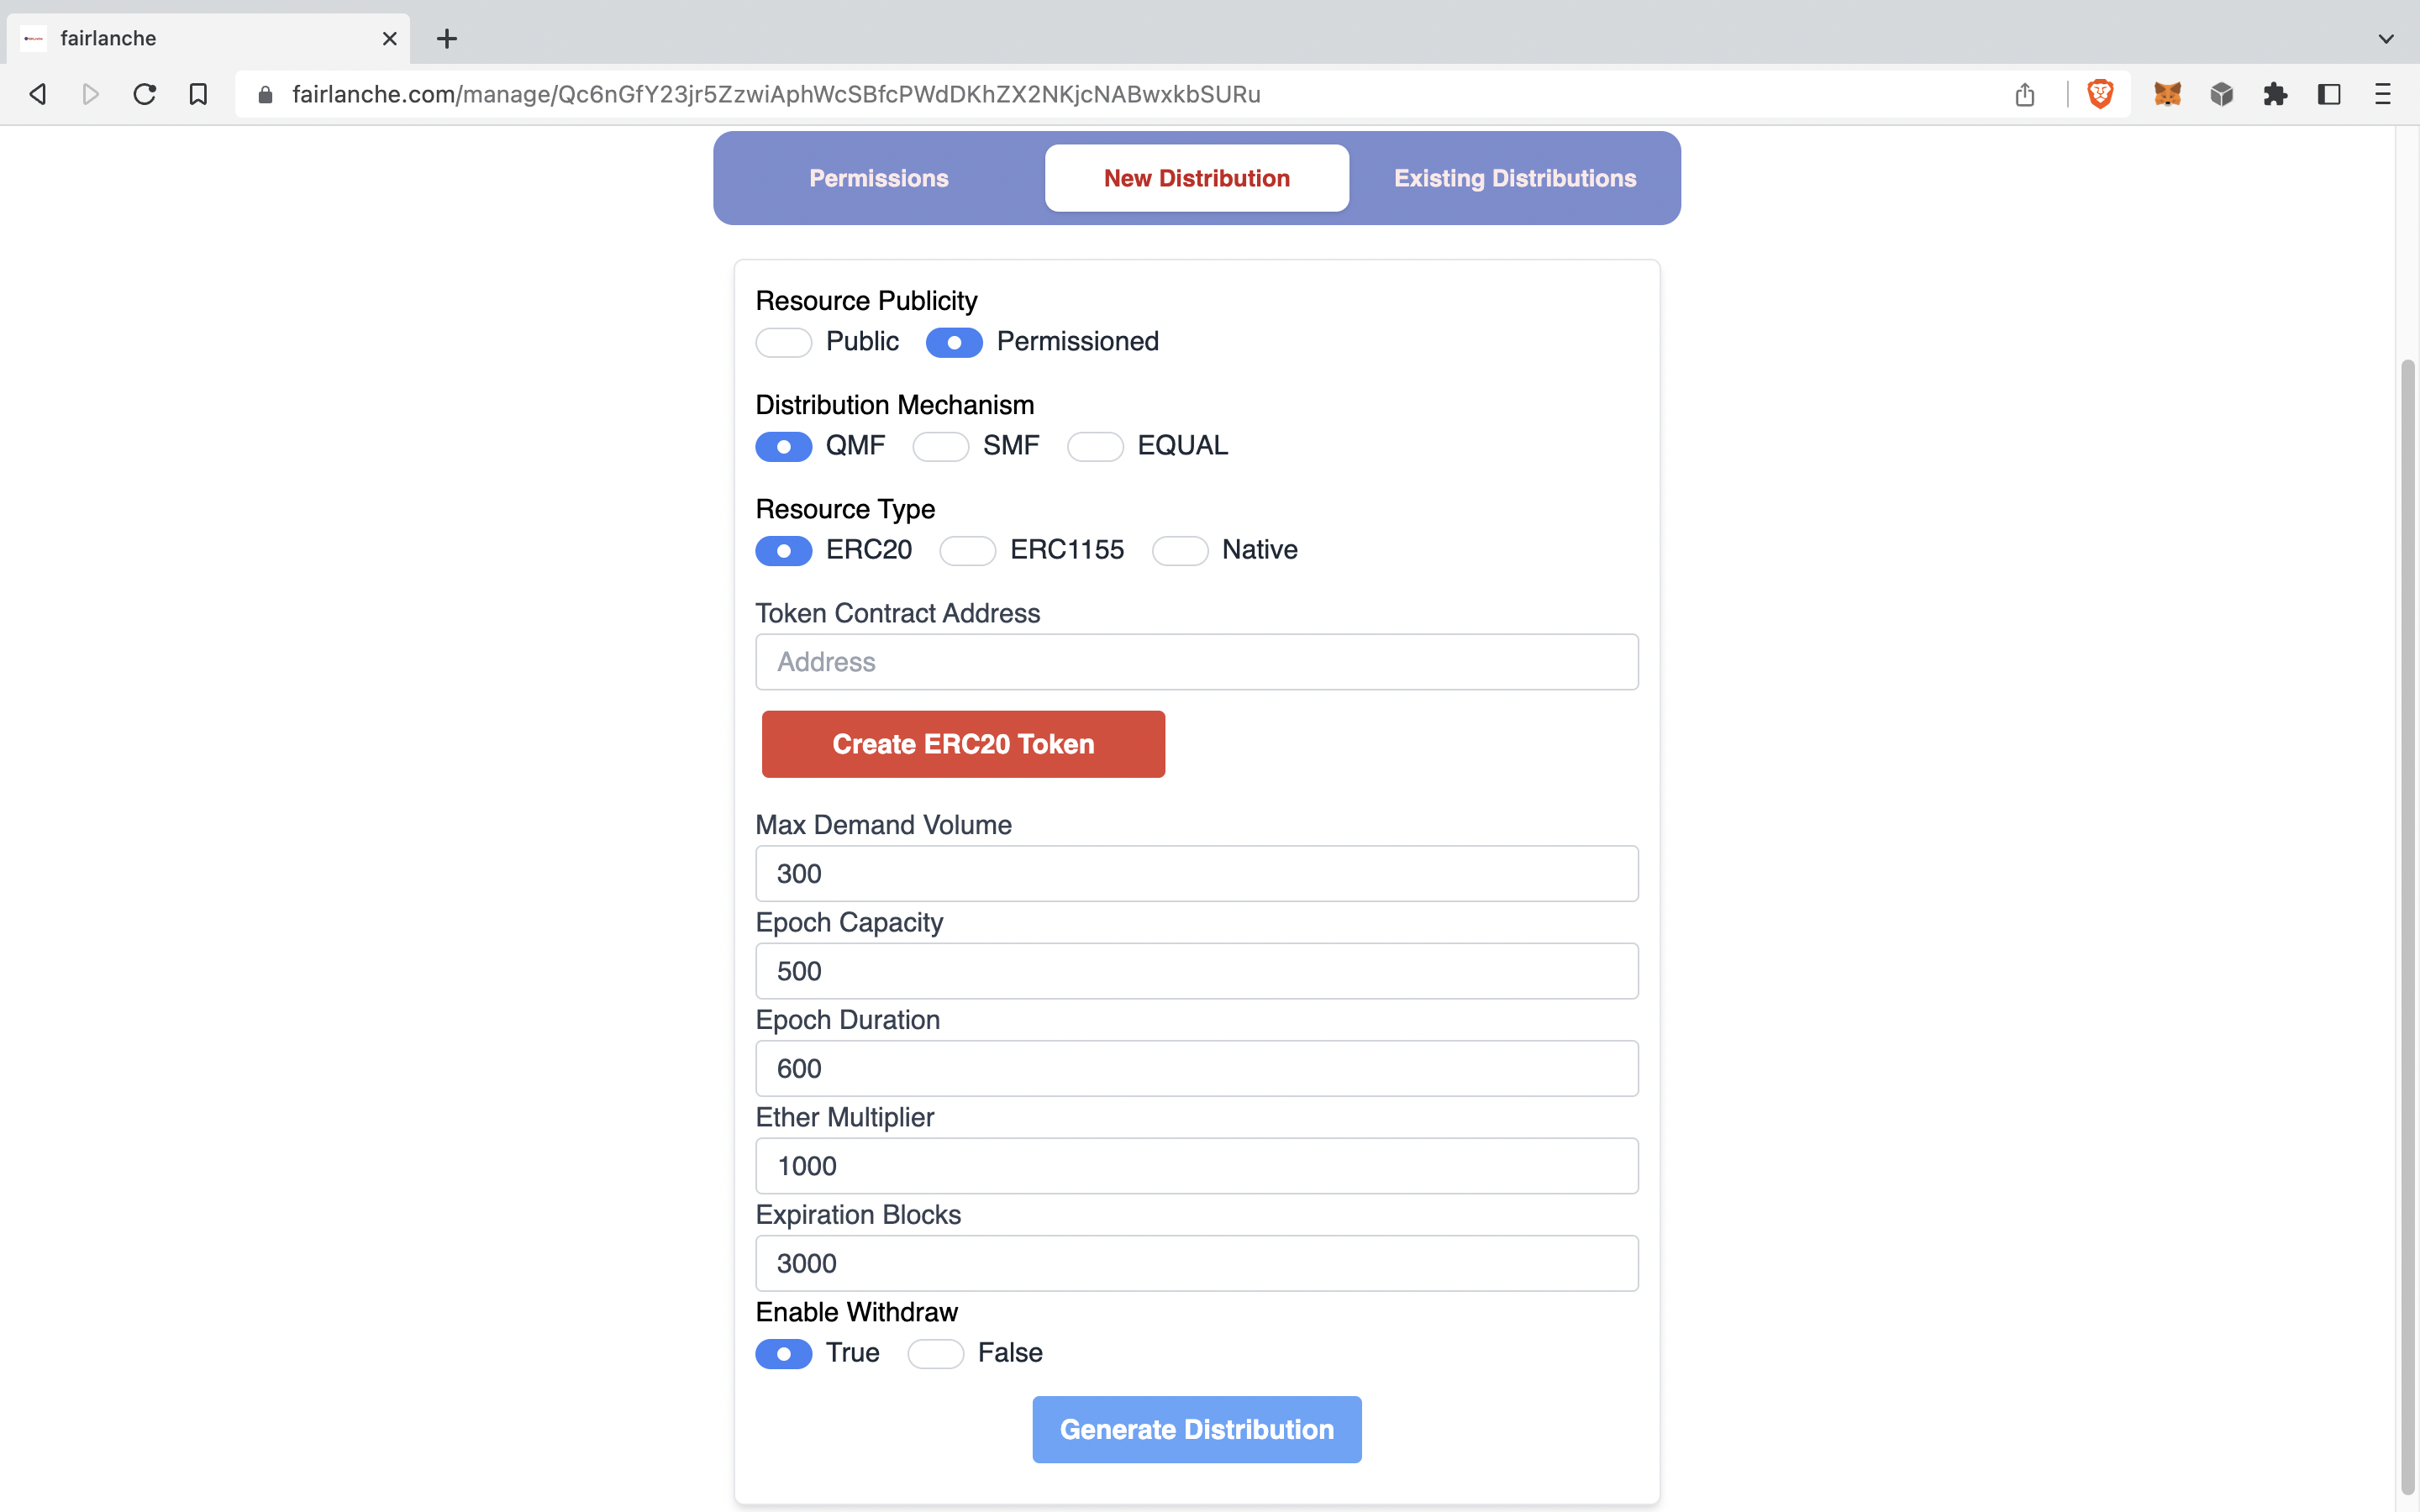
\includegraphics[width=1\textwidth]{ss7.png}
	\caption{ERC20 Distributor Deploy UI}
\end{figure}
\begin{figure}[H]
	\centering
	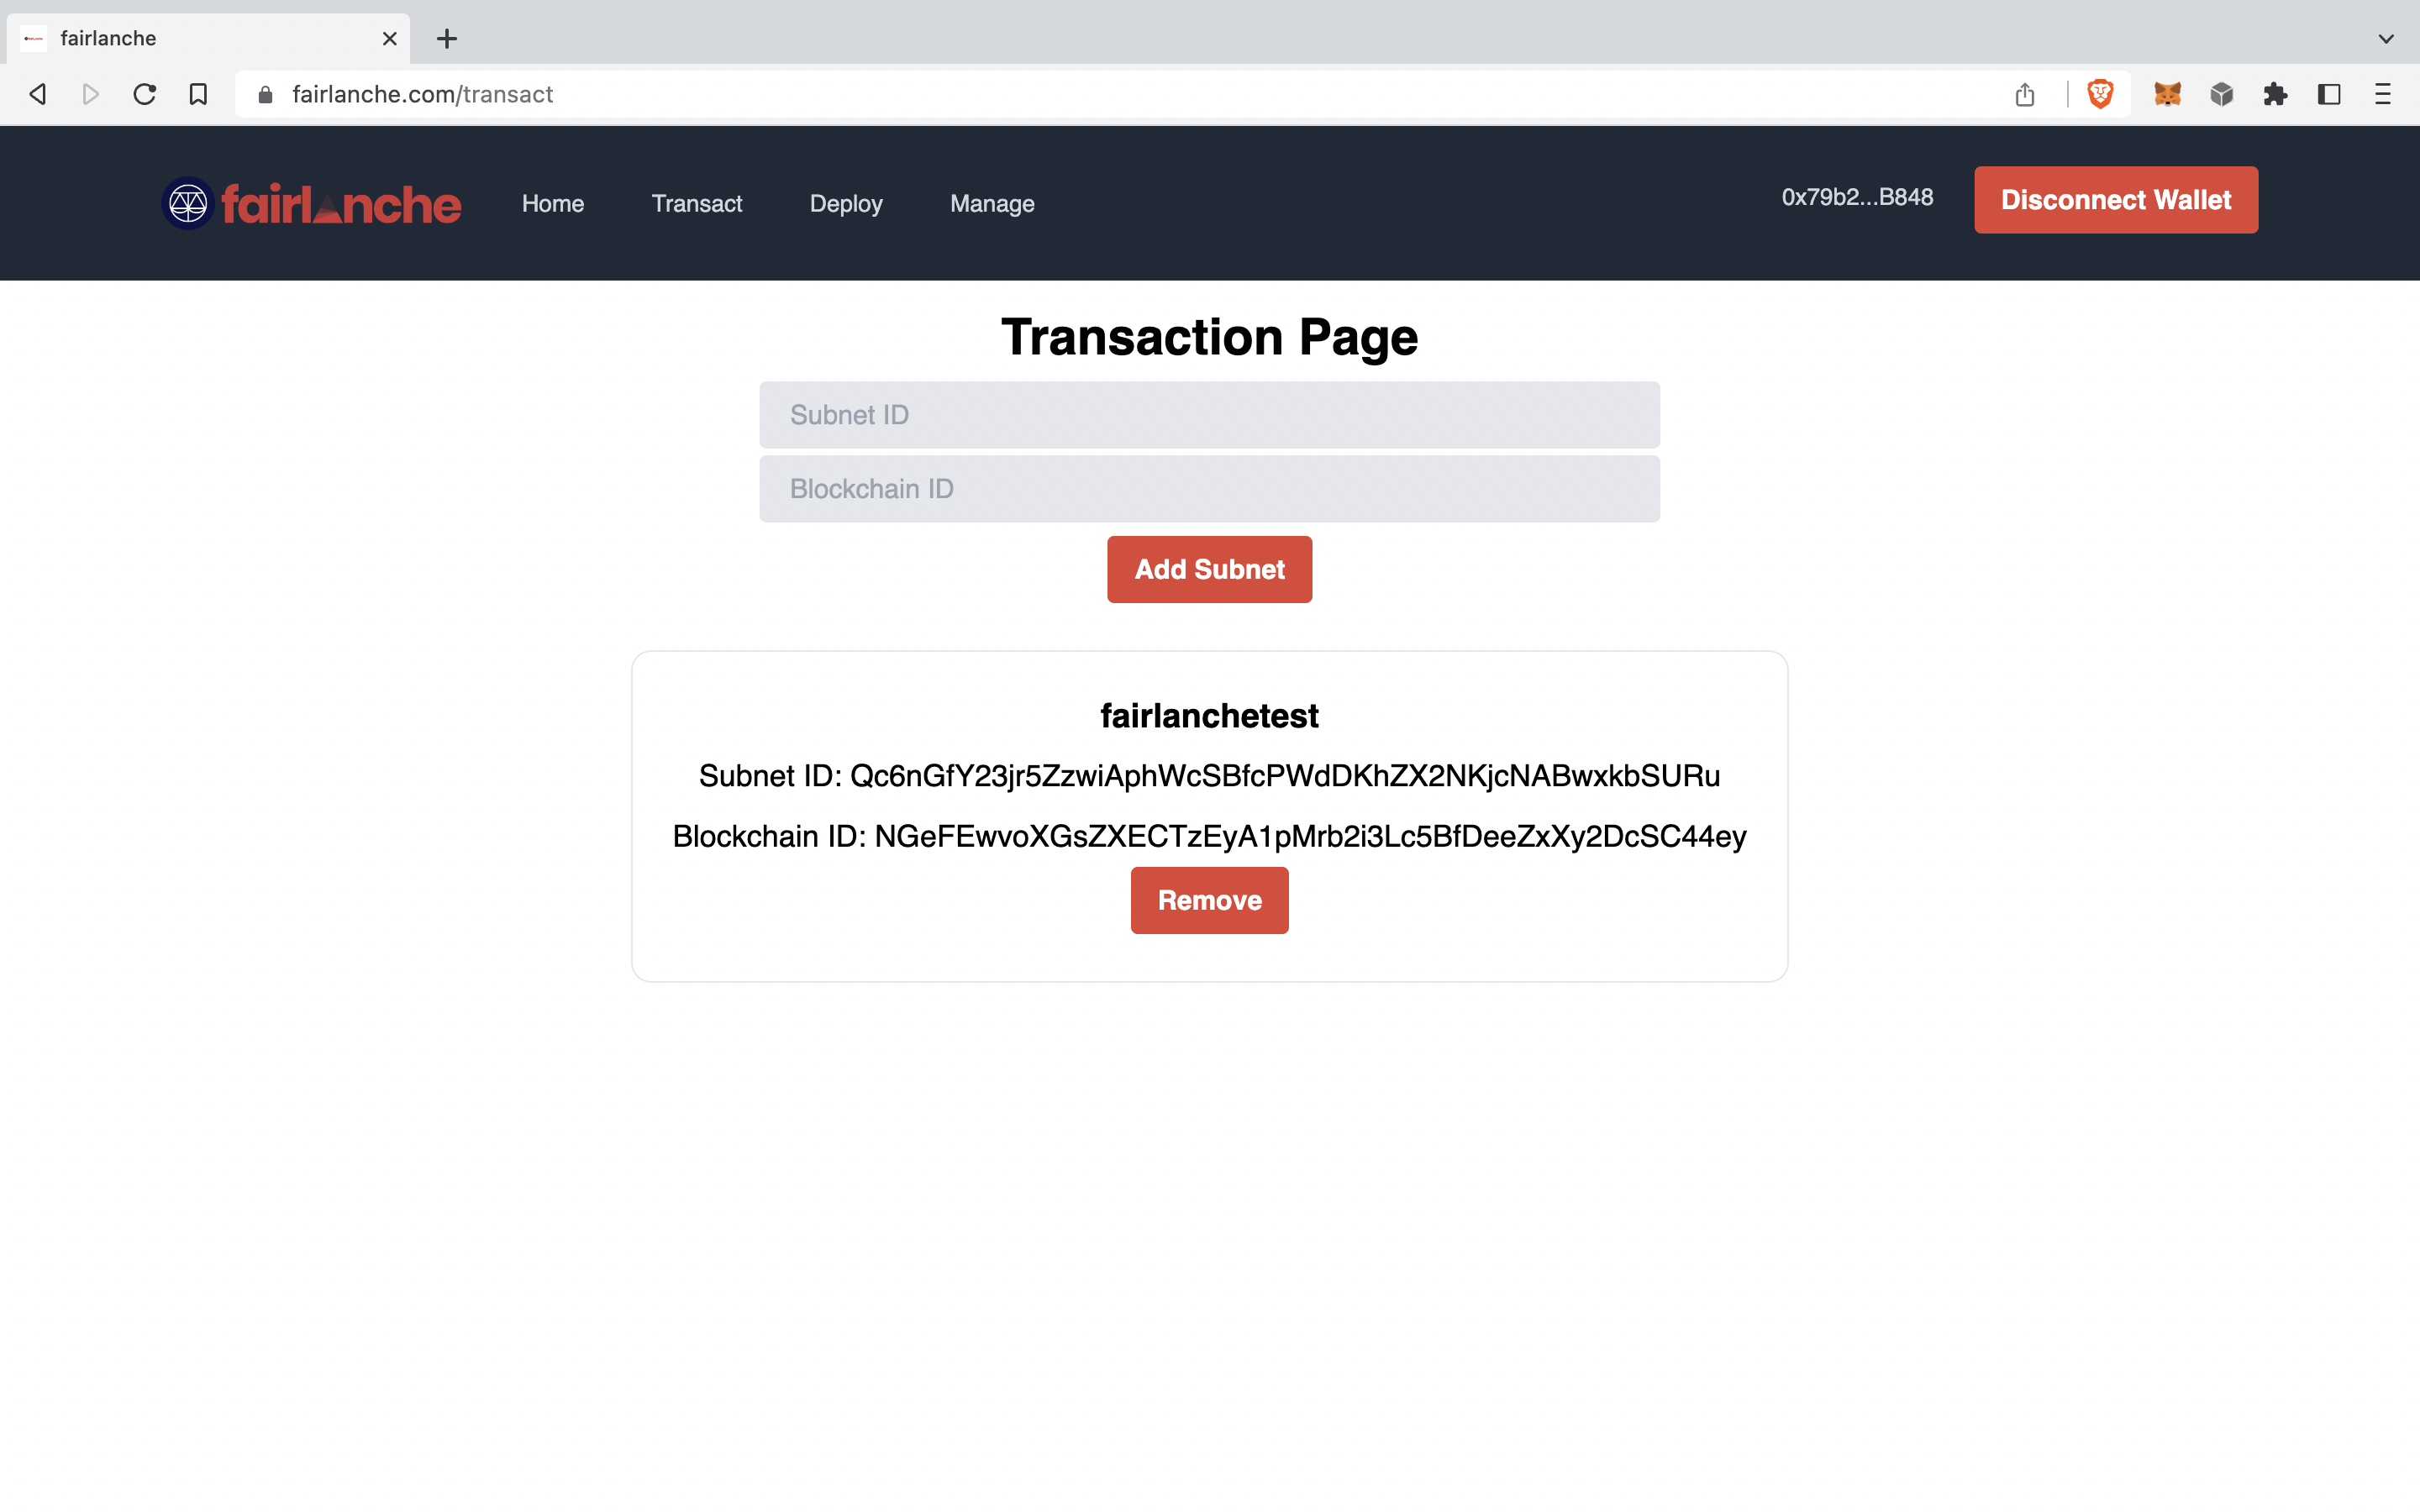
\includegraphics[width=1\textwidth]{ss8.png}
	\caption{Distribution Management UI}
\end{figure}
\subsection{Tranasction Page}
\begin{figure}[H]
	\centering
	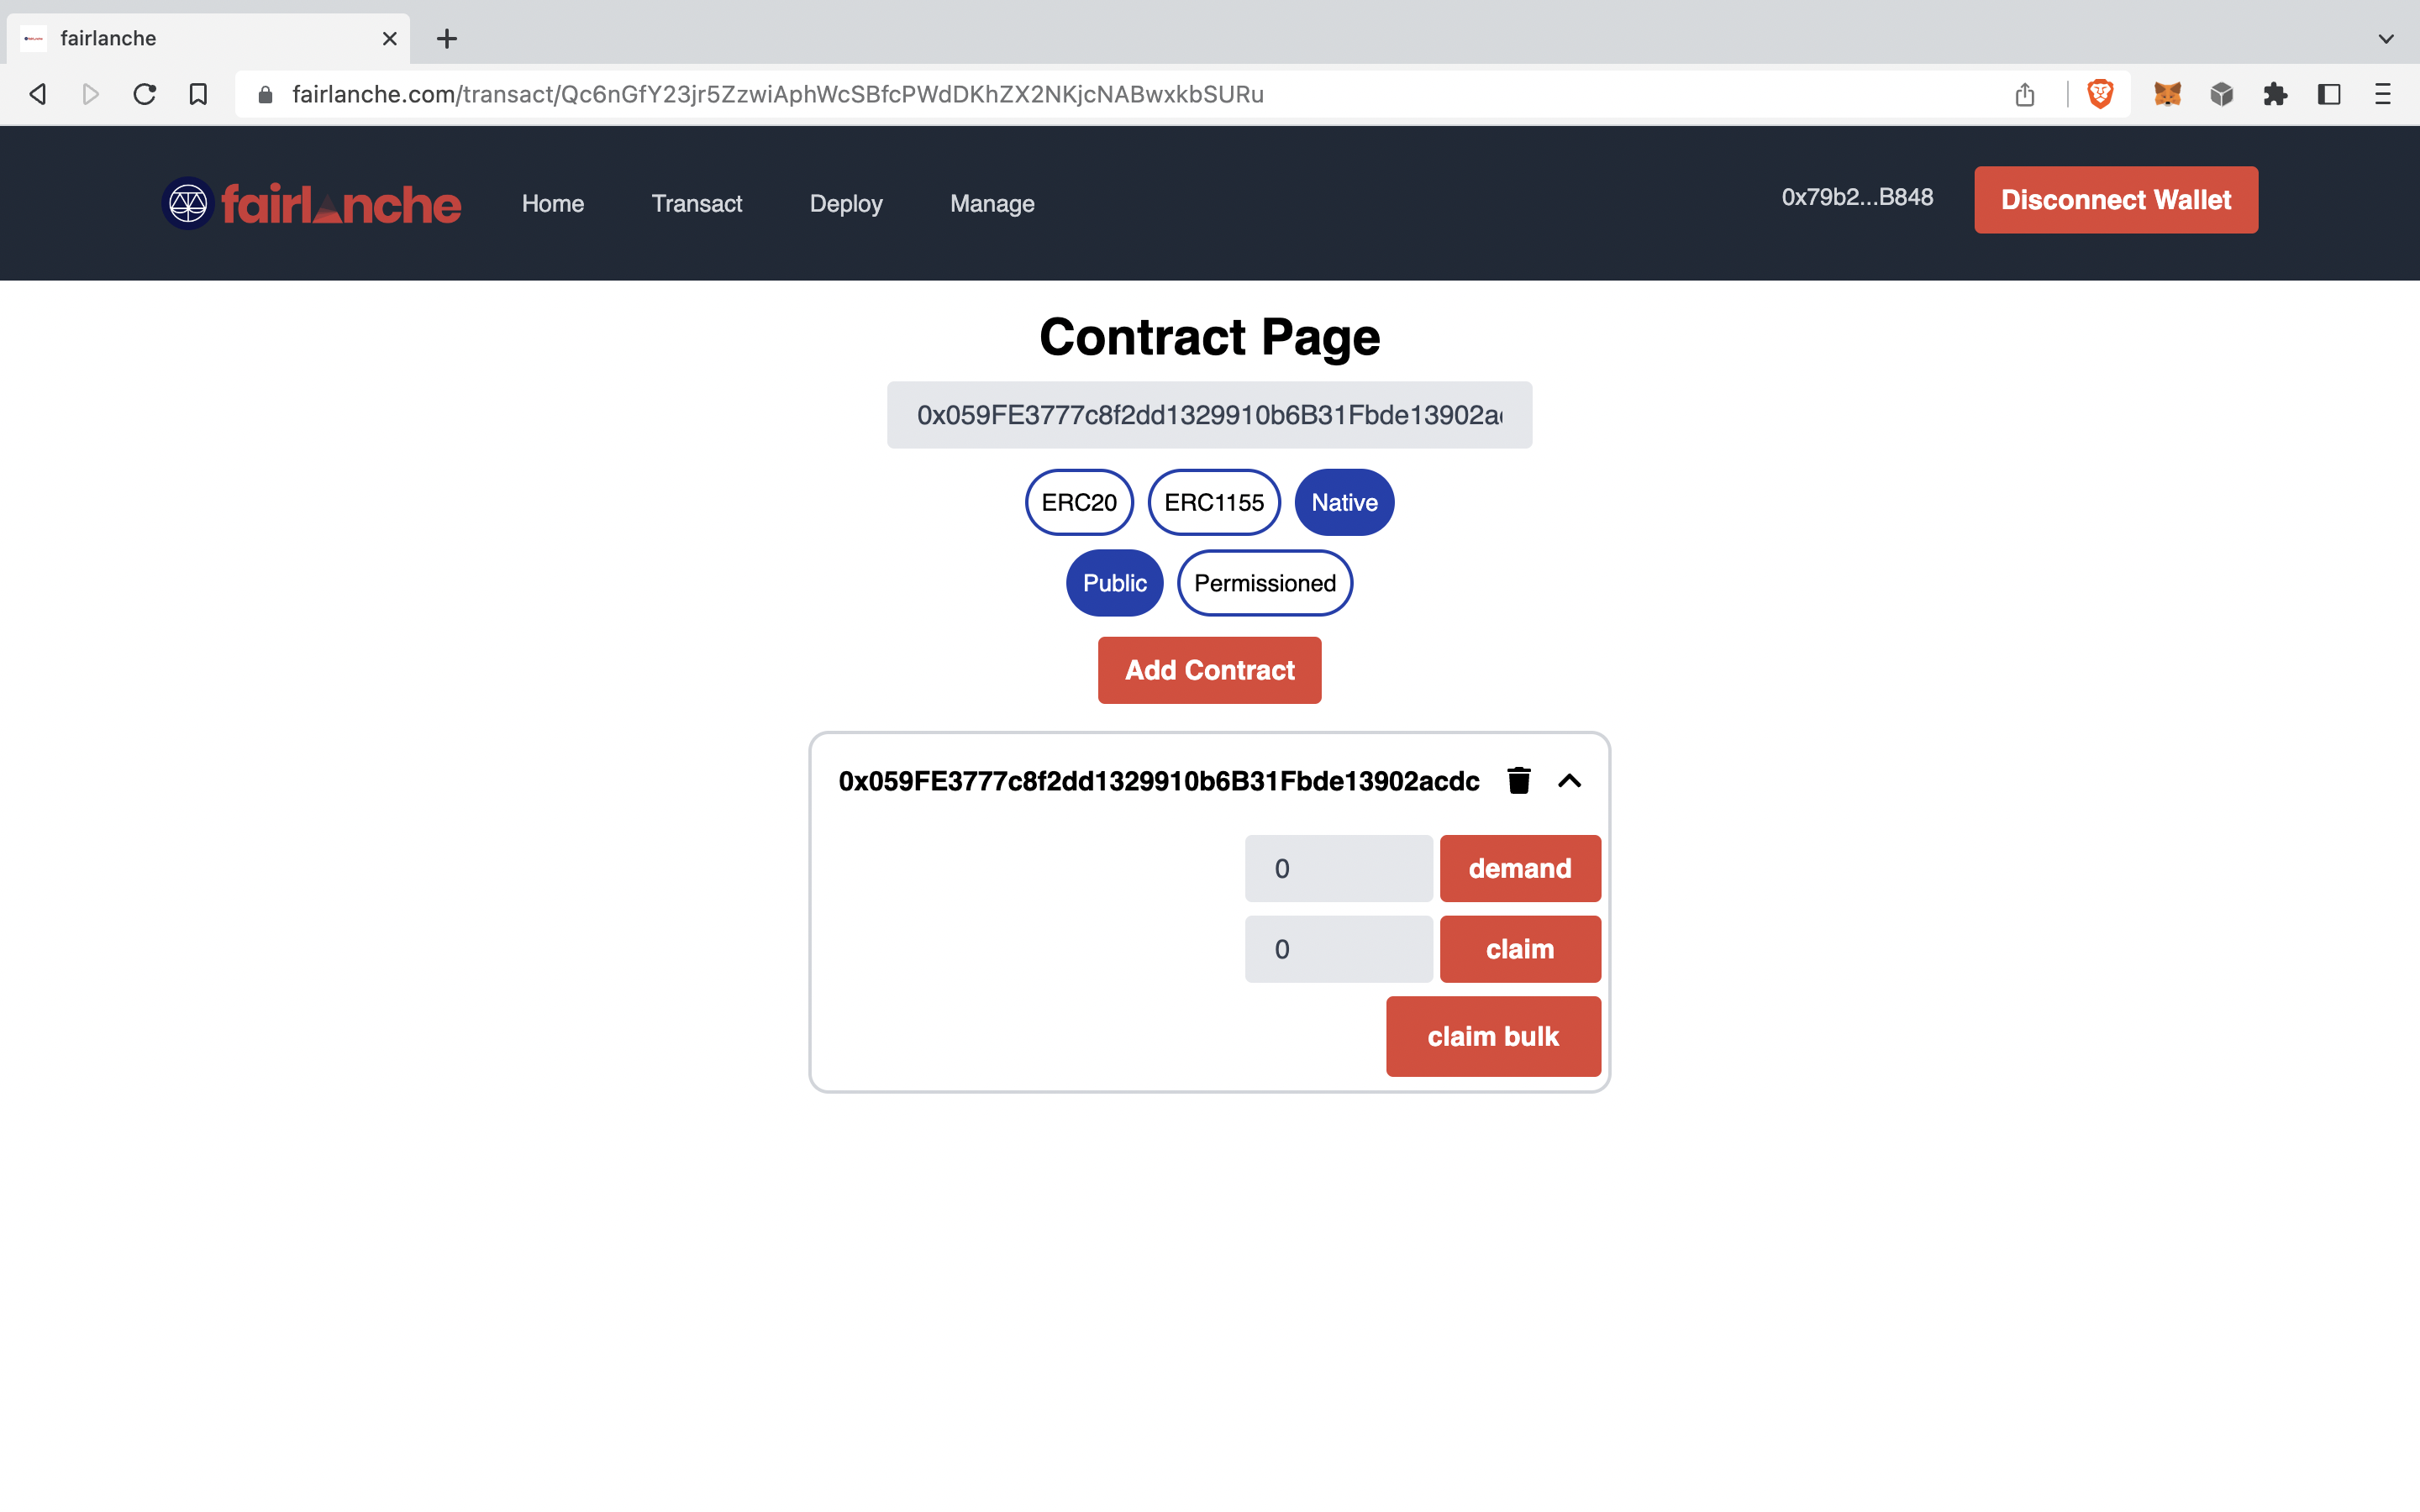
\includegraphics[width=1\textwidth]{ss9.png}
	\caption{Transaction Page UI}
\end{figure}

\begin{figure}[H]
	\centering
	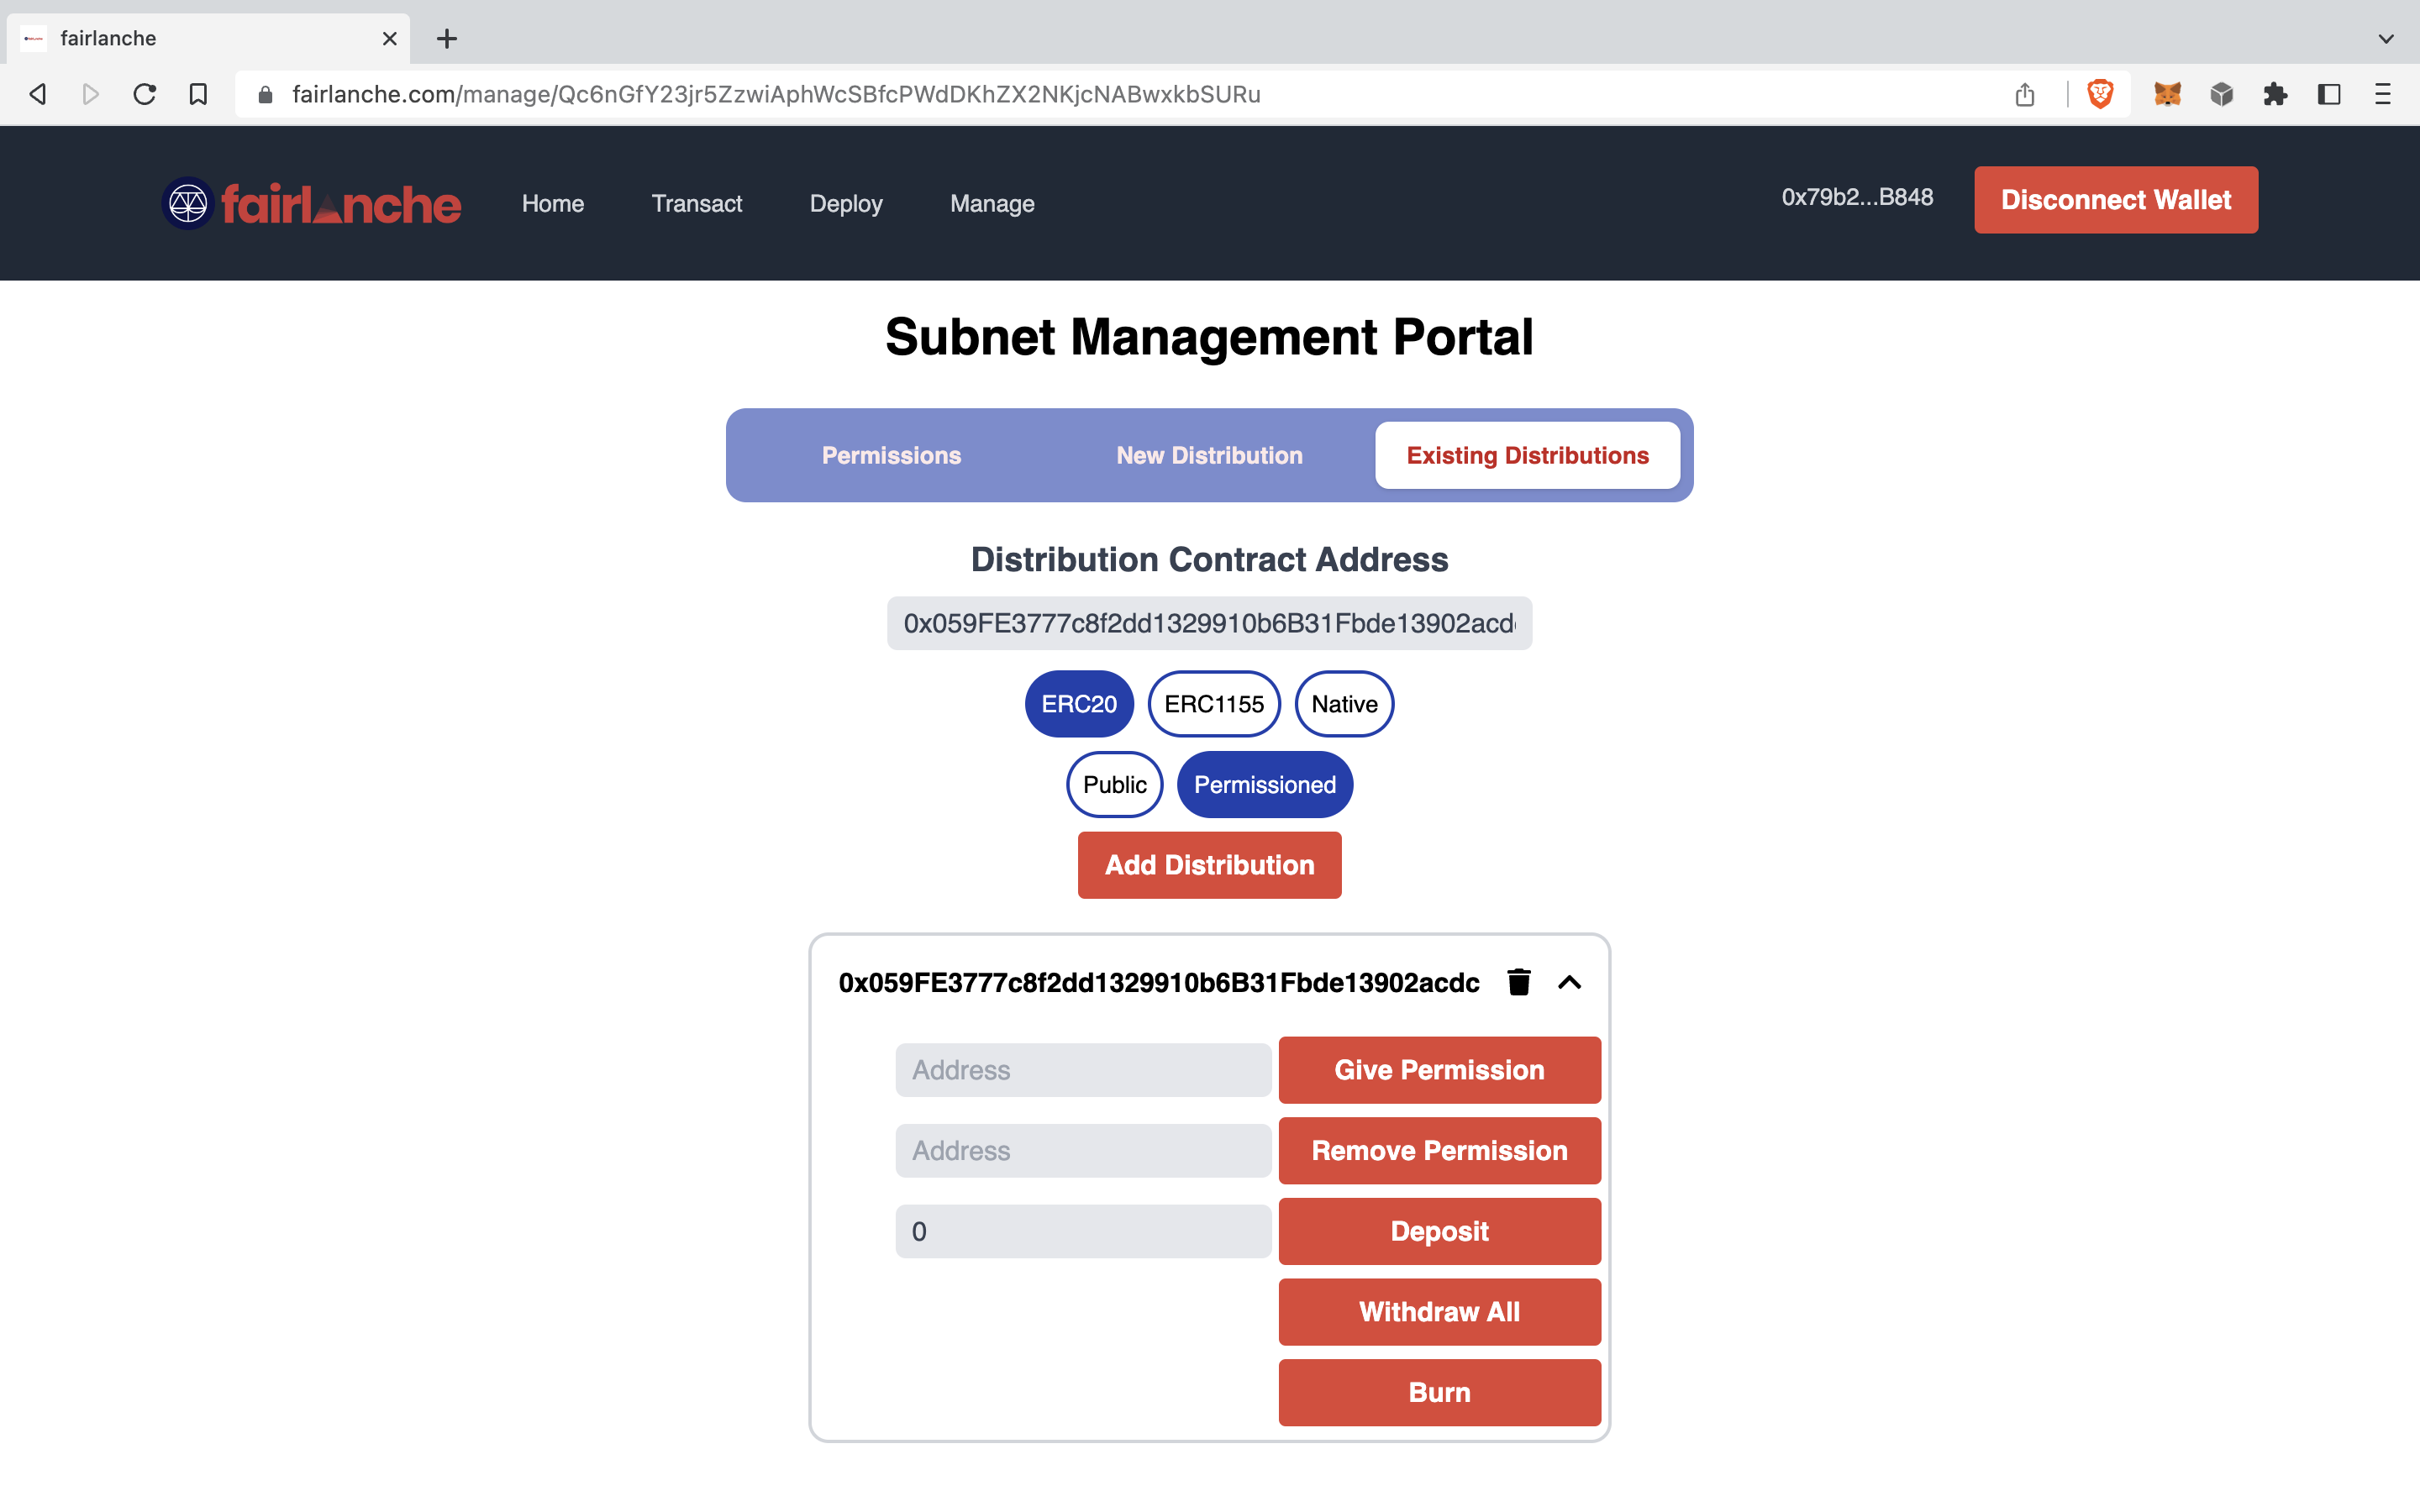
\includegraphics[width=1\textwidth]{ss11.png}
	\caption{Contract Page UI}
\end{figure}

\chapter{IMPLEMENTATION AND TESTING}
\section{Implementation}
\subsection{Handling P-Chain Transactions}
Since our application only provides interactions with Metamask, the user could only interact with Avalanche’s EVM-compatible C-Chain. However, creating subnets and blockchains are only possible on P-Chain. To resolve this problem, we utilized the AvalancheJS library and handled the P-Chain transactions behind. 

First of all, the initial task was to fund the user’s P-Chain wallet. For this, we made a cross-chain transfer from C-Chain to X-Chain, and then X-Chain to P-Chain. We used exportAVAX and importAVAX endpoints from P-Chain API to handle these atomic transactions. The user “exported” some AVAX with their signature on Metamask, and our application handled the rest by importing this balance to P-Chain.

All the other functions we used with Avalanche’s API were very self-explanatory. Using createSubnet, addSubnetValidator and createBlockchain endpoints were sufficient to provide the user with the necessary functionality on P-Chain.

\subsection{Deploying Subnets}
Deploying subnets and assigning validators to them is one of the fundamental functionalities of our application. The resources to be distributed on custom blockchains will exist on the subnets that are validated by the community. 
\newpage
The user can send a request for creating a new subnet and adding a validator afterwards. To use addSubnetValidator endpoint, the user has to enter a Node-ID but we assign them our node. We obtained our Node-ID from calling the getNodeId from Avalanche’s info API.

\subsection{Creating Customized Blockchains}
In Avalanche’s P-Chain API, creating blockchains requires a genesis data that contains information about the initial state of the virtual machine. This data includes many parameters from the newly created blockchain’s chainID, name, asset allocation at the beginning of the new blockchain, to its gas configurations.

In the platform, the user enters these values to text input fields and we arrange the information according to the expectations of the createBlockchain endpoint, using our buildGenesis utility function.

Additionally, the application also allows users to further customize their blockchains by adding precompiles for restricting the allowances on them. It is possible to restrict both contract deployers and transactions on the created blockchain separately. Users can activate these precompiles by providing lists of Enabled and Admin addresses for those.

The list of addresses (TxAllowList) that are allowed to transact on the blockchain will exist in the precompiled contract at 0x0200000000000000000000000000000000000002 whereas the DeployerList will be at 0x0200000000000000000000000000000000000000. The state of those could be updated by the Admin addresses provided in the related address list, hence, providing a dynamic way to manage blockchain-scoped permissions.

\subsection{Resource Distribution Contracts}
We fundamentally implemented the abstract contracts ResourceDistributor and PResourceDistributor, which inherits from the former, as our base contracts. Every other resource contract has inherited from those.

Most of the contract state management took place in ResourceDistributor whereas the share calculations (and therefore the implementations of the distribution algorithms mentioned in the report) took place in pure functions under ShareCalculator. 

In ResourceDistributor, the time is divided into epochs to represent a time period of constant number of blocks. It also includes the fundamental demand(), claim(), and claimAll() functions that are pretty self-explanatory when they are considered with the system models provided in previous sections. Basically, the Permissioned User makes a demand by calling demand(volume)with the unit of resources that they would like to receive. Then, they may claim their shares after the epoch that they made the demand is over by calling claim(epochNumber)providing the epoch number that the demand was made. Alternatively, they may wait for some more epochs, and they can claim all of their pending shares by calling claimAll()at once.

updateState() function checks whether the current epoch is over. If the latest epoch is over, then it calculates the share for it by calling the calculateShare() function. Afterward, the share of that epoch is recorded in the shares[] array and then, each user can claim their shares according to the chosen distribution policy.

In our project, we enhanced the implementation by Metin S., Ozturan C., that enforces the users to claim their shares in the next epoch. Since both the shares[] array and users’ demands are never looped, we could store them all since the very first epoch. Therefore, users could claim their shares any time, unless the distribution is over.

\newpage 

On the other hand, ShareCalculator includes three functions that calculate the share with QMF, SMF, or a simple distribution algorithm, that is Equal Distribution. The ShareCalculator library is independent of the state of the blockchain as all of its functions are pure. Thus, it is possible to integrate more distribution algorithms into this project.

The QMF and SMF algorithms are implemented as they are described in Quantized and Simulated Max-min Fairness in Blockchain Ecosystems, utilizing the pseudocodes provided.


The Equal Distribution Algorithm on the other hand, calculated the share with the following formula:

\begin{figure}[H]
	\[
	equalShare = cumulativeCapacity / totalDemand
	\]
\end{figure}

At the end of the epochs, users who have demands can claim the minimum of their demands and the calculated equalShare.

Using these base contracts, we created many variations for different assets, policies and allowance options thanks to inheritance. The final directory structure for the contracts can be seen below:

\begin{figure}[H]
	\centering
	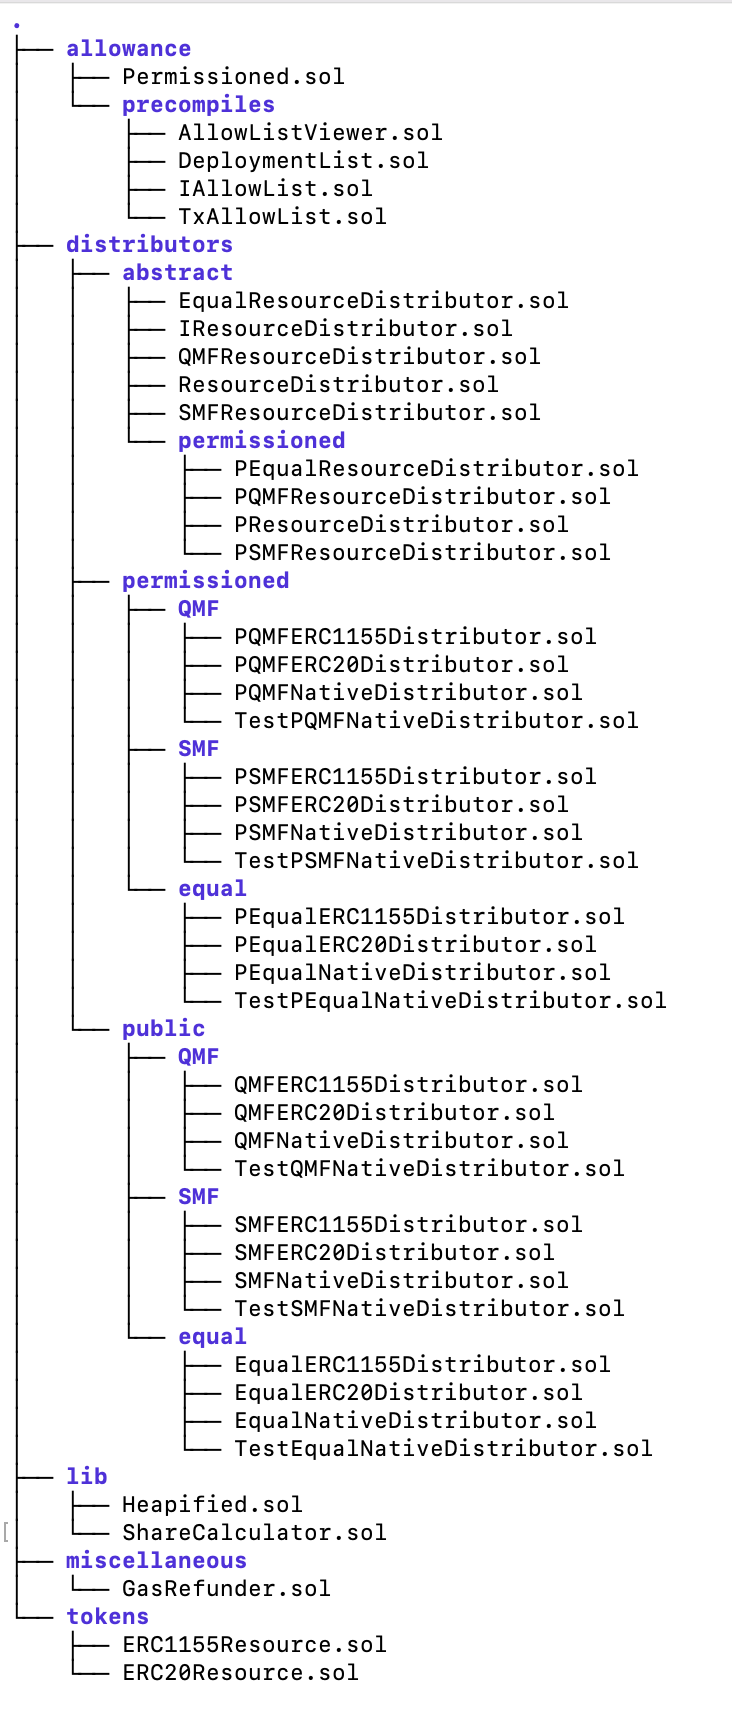
\includegraphics[width=0.5\textwidth]{dir.png}
	\caption{Contract Directory Structure}
\end{figure}

We also connected our smart contract implementations to the front-end so that users could interact with the existing contracts, update them or deploy new ones using the management panel.

\section{Testing}
\subsection{Test Cases}
We used Hardhat tests for the testing process of our smart contracts. Our test cases were comprehensive and sufficient to test our complex contract structure. We tested all resource types: ERC20, ERC1155, and the Native Asset distributors. Also, we wrote test cases for different distribution algorithms and permission options. 

In total, we had 147 different successful test cases testing contracts’ functionality with various scenarios.

These test cases mainly focused on the points below for different resource, distribution algorithm and allowance options:

\begin{figure}[H]
	\centering
	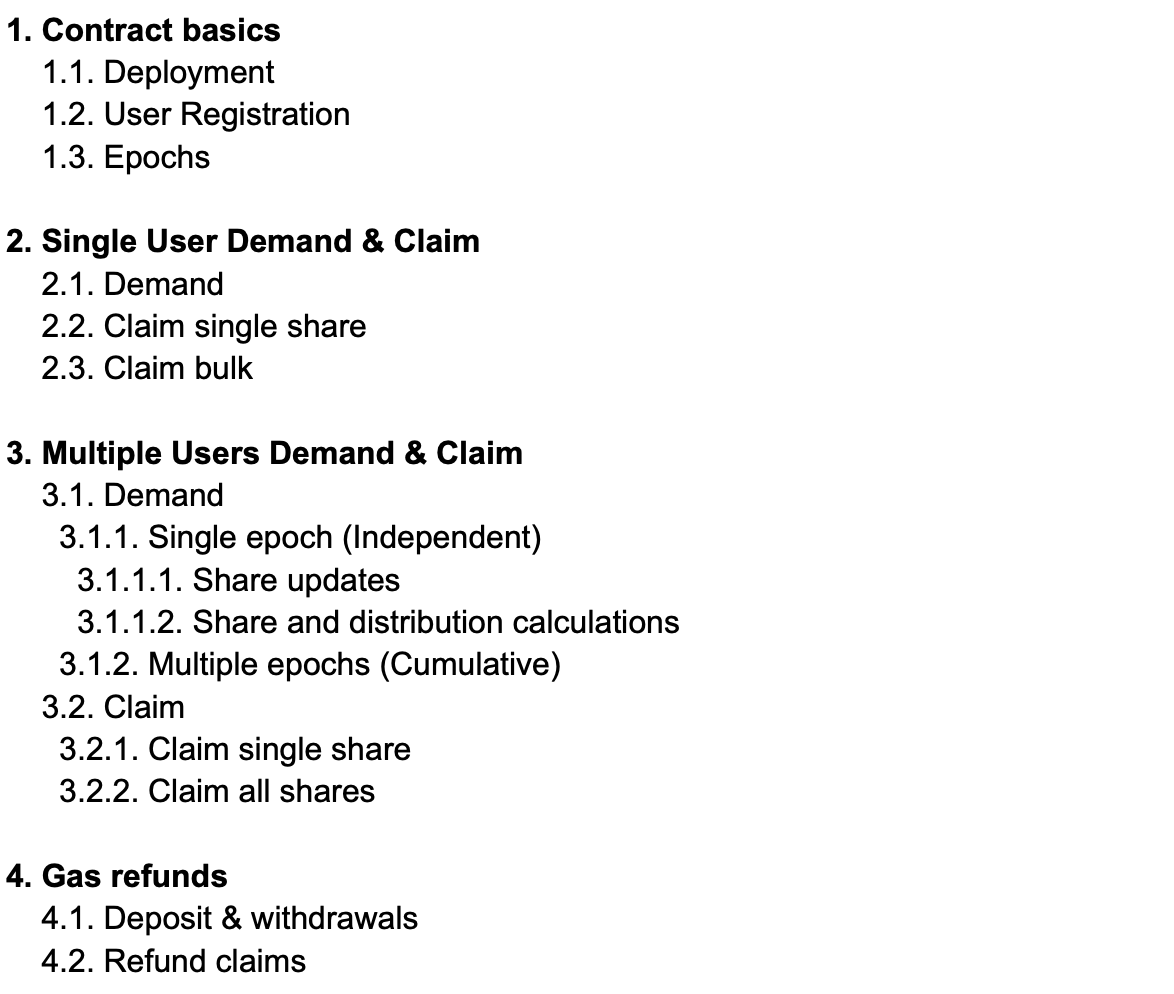
\includegraphics[width=0.8\textwidth]{tests.png}
\end{figure}

\subsection{Gas Reports}
The functions that do not grow with the maximum number of demands are not included in the gas reports as they are not an issue for scaling. Also we did not generate gas reports for different resource types and allowance options as they will be very similar to those below.

\begin{figure}[H]
	\centering
	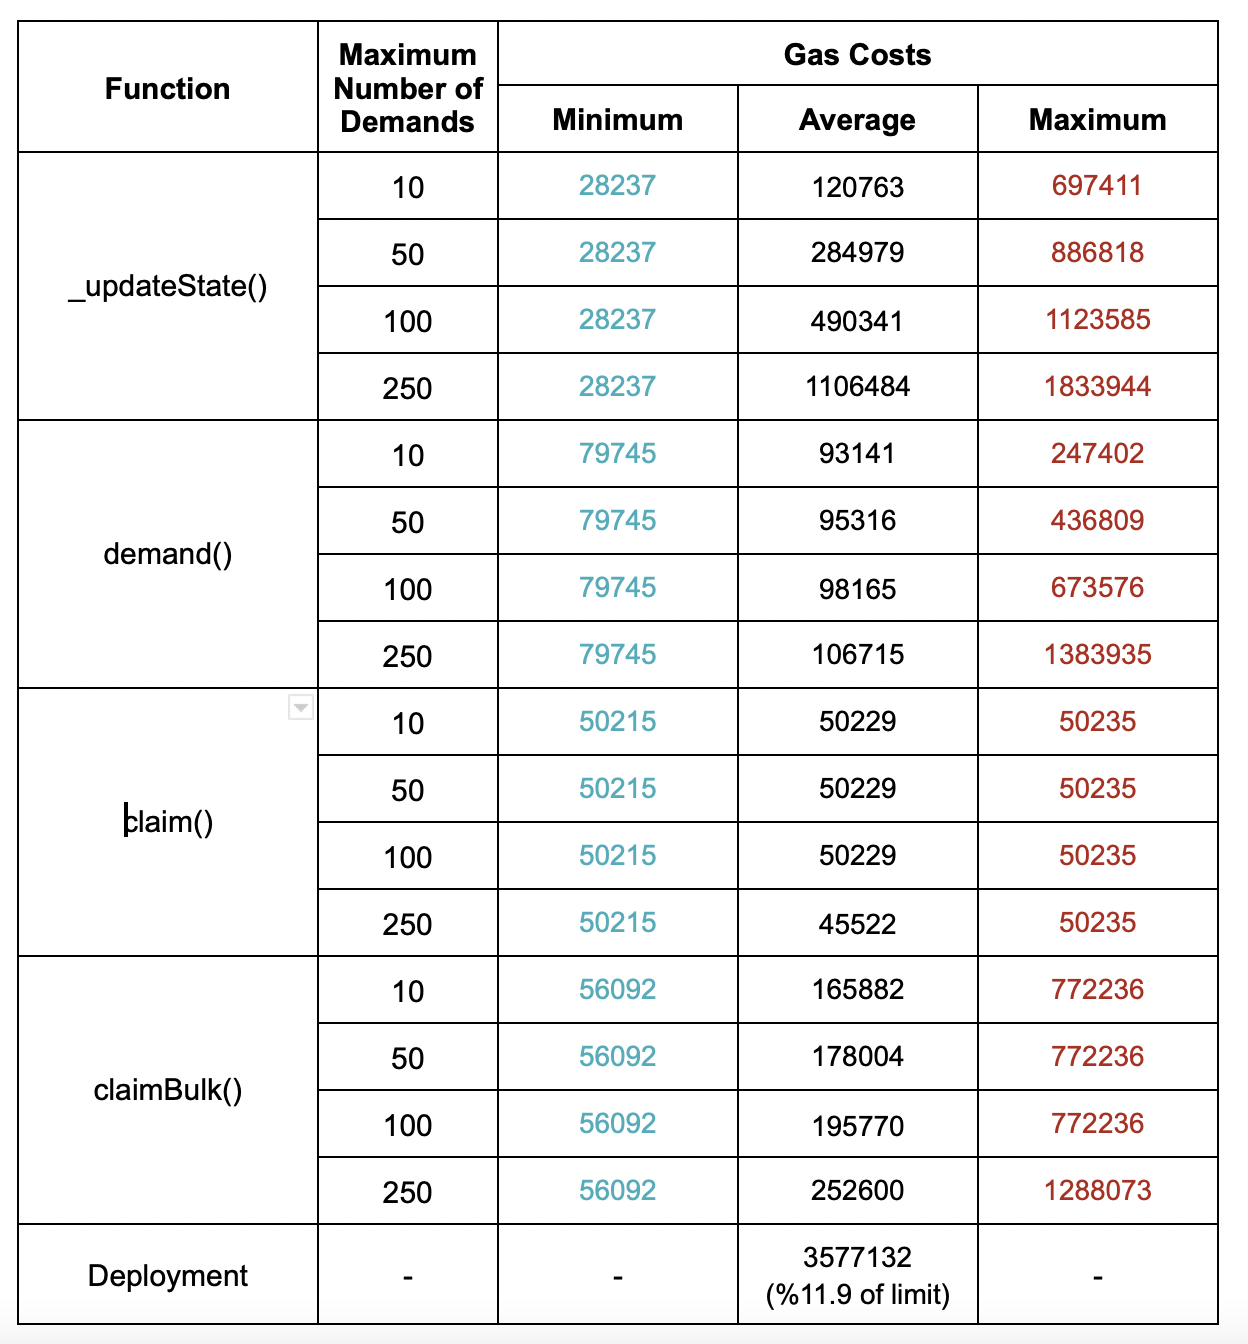
\includegraphics[width=1\textwidth]{gas_table.png}
	\caption{Gas Table}
\end{figure}

\textbf{Solidity Compiler Version}: 0.8.17,
\textbf{Run Count for Average Calculations}: 200,
\textbf{Optimizer}: Not Enabled,
\textbf{Demand Expiration Time}: 100

\section{Deployment}
\subsection{Deployed \& Verified Smart Contracts}
We have created all types of resource distribution contracts on Fuji network and verified them on Snowtrace, a blockchain explorer for Avalance’s C-Chain. Additionally, we deployed Allowance contracts and the ShareCalculator library as well.

All contracts can be viewed and their source code can be verified in the following links:
\\
\textbf{Native Asset Distributors}
\begin{itemize}
	\item \href{https://testnet.snowtrace.io/address/0xf3511AC9c42b52D2728722DFE14486E849897b83}{QMFNativeDistributor}
	\item \href{https://testnet.snowtrace.io/address/0x080f7c0aa98e4ef3f3fa441cf8728277932f8f92}{SMFNativeDistributor}
	\item \href{https://testnet.snowtrace.io/address/0x8926df2df0bb310d978961c76375b936b4b3c1e2}{EqualNativeDistributor}
	\item \href{https://testnet.snowtrace.io/address/0x5feEAB0162c5aFFB98E7c346f33B9FC18777F3cA}{PQMFNativeDistributor}
	\item \href{https://testnet.snowtrace.io/address/0x5842c0814EbA6eECB9c8B61ff58C077B20eF46b1}{PSMFNativeDistributor}
	\item \href{https://testnet.snowtrace.io/address/0xD136D5138c87CCD300fB88692616db7bf50E24c1}{PEqualNativeDistributor}
\end{itemize}

\newpage

\textbf{ERC20 Distributors}
\begin{itemize}
	\item \href{https://testnet.snowtrace.io/address/0x960E76607E554ef13e95Bb02316D7e45e62b9CA6}{QMFERC20Distributor}
	\item \href{https://testnet.snowtrace.io/address/0xCd6FecCE500548D7e01bC0bD343ee25Bc99b6a18}{SMFERC20Distributor}
	\item \href{https://testnet.snowtrace.io/address/0xe21C63cC67eb20Ce187f1E9C1B853E23CA47e539}{EqualERC20Distributor}
	\item \href{https://testnet.snowtrace.io/address/0xbd8fC81BfF7a73618abafF6e2812541F8f1a7186}{PQMFERC20Distributor}
	\item \href{https://testnet.snowtrace.io/address/0xEbd643f47D669FBC427C102f981E6EC9E87e99de}{PSMFERC20Distributor}
	\item \href{https://testnet.snowtrace.io/address/0xB64a91bc12dB15B98ab002Cc628165842A1a0193}{PEqualERC20Distributor}
\end{itemize}

\textbf{ERC1155 Distributors}
\begin{itemize}
	\item \href{https://testnet.snowtrace.io/address/0x7CC306949b2908b543377268e8F98865a72BDb93}{QMFERC1155Distributor}
	\item \href{https://testnet.snowtrace.io/address/0xA497D8079dE4E323361e119A3d540113f051A0DB}{SMFERC1155Distributor}
	\item \href{https://testnet.snowtrace.io/address/0x870921CEE8465B9920A904ff762d605eC0d929Fb}{EqualERC1155Distributor}
	\item \href{https://testnet.snowtrace.io/address/0x1f409a3848Ce2052c15e5AD94419aF4c7819E96F}{PQMFERC1155Distributor}
	\item \href{https://testnet.snowtrace.io/address/0xc09D7EAdfaE4f1E80D04D52113B8767322fDB9eC}{PSMFERC1155Distributor}
	\item \href{https://testnet.snowtrace.io/address/0x169548d82919Db3aD3cE037277DD450447858e90}{PEqualERC1155Distributor}
\end{itemize}

\textbf{Libraries}
\begin{itemize}
	\item \href{https://testnet.snowtrace.io/address/0x3e388dd91ce0714c427bad7ad128fbfc588b2ae2}{Heapified}
	\item \href{https://testnet.snowtrace.io/address/0x30fbd74b5ea995a279416c16e02f281bb478837b}{ShareCalculator}
\end{itemize}

\textbf{Allowance Contracts}
\begin{itemize}
	\item \href{https://testnet.snowtrace.io/address/0x0f8cfd4d5a0807d3f9f0a29afd52b9b5b6db6e37}{DeploymentList}
	\item \href{https://testnet.snowtrace.io/address/0xa14b962542b3f0518cd89dd93ecc86ba53b3d371}{TxAllowList}
\end{itemize}

\textbf{Resource Contracts}
\begin{itemize}
	\item \href{https://testnet.snowtrace.io/address/0xcd1c77b27f488bb225b1c604629918d0240c2c3a}{ERC20Resource}
	\item \href{https://testnet.snowtrace.io/address/0x38A244Ef32099fB90C15D22c1BEE33bE14d185bF}{ERC1155Resource}
\end{itemize}

\subsection{Running a Fully Bootstrapped Fuji Node}
As mentioned earlier, we developed a gateway to access both Avalanche’s EVM-compatible C-Chain and P-Chain for new blockchain deployments. Therefore, we did not store any user information, anywhere. No databases were used in the development. Users simply interacted with the blockchain directly through the node.

In order to provide this functionality, we ran a Fuji node ourselves and pointed it at \href{https://fairlanche.link:9650}{fairlanche}. Users accessing our application in our front-end simply interact with this node and send their transactions.

We also promoted this node to be Validator in Avalanche’s Primary Chain on Fuji network by staking the necessary AVAX. Also, we fully bootstrapped it and provided necessary VM images for compilation so that it could be a Subnet Validator for the newly created subnets via our platform.

\subsection{ React App Deployment on ECS}
We built our application using Docker. It is possible to run the app by cloning the repository and running the docker-compose up command in the docker directory. We uploaded this image to AWS’s ECR, built a task with it and ran it with ECS.

We also handled the TSL certificates, and the final deployed React App can be found at  \href{https://fairlanche.com/}{fairlanche.com}.

\subsection{Summary}
\begin{table}[H]
	\begin{tabular}{|c|c|}
		\hline
		\textbf{Deployed Software} & \textbf{Link}                           \\ \hline
		Verified Smart Contracts   & Check 7.3.1 for the full list           \\ \hline
		Avalanche Fuji Node        &  \href{https://fairlanche.link:9650}{https://fairlanche.link:9650}.           \\ \hline
		Fairlanche Application     & \href{https://fairlanche.com/}{fairlanche.com}.               \\ \hline
		Github Repository          & \href{https://github.com/canatakan/fairlanche}{https://github.com/canatakan/fairlanche}.    \\ \hline
	\end{tabular}
\end{table}

\subsection{Build Instructions}
The project is provided with well-detailed README files for the hardhat-project, subnet and front-end modules. The instructions are sufficient to build the application on local environments. Before applying any instructions, firstly clone the repository including its AvalancheJS git submodule.
\begin{itemize}
	\item 
	The easiest way to run the front-end application is to run the docker-compose up command in the docker directory. The server will be online at port 3000.
	\item 
	To build the front-end application without docker, go to the avalanchejs directory and build the app as explained in the README file of the enclosing folder. 
	\item 
	Then, go to the subnet/front-end and front-end directory and install dependencies by using npm install. 
	\item 
	Update the create-react-app’s configurations as explained in its README to add necessary fallbacks. Then install the dependencies again.
	\item 
	For building the Hardhat project and updating or interacting with the existing smart contracts, simply run npm install in the hardhat-project directory.
\end{itemize}
\newpage
\subsection{Deployment Diagram}
\begin{figure}[H]
	\centering
	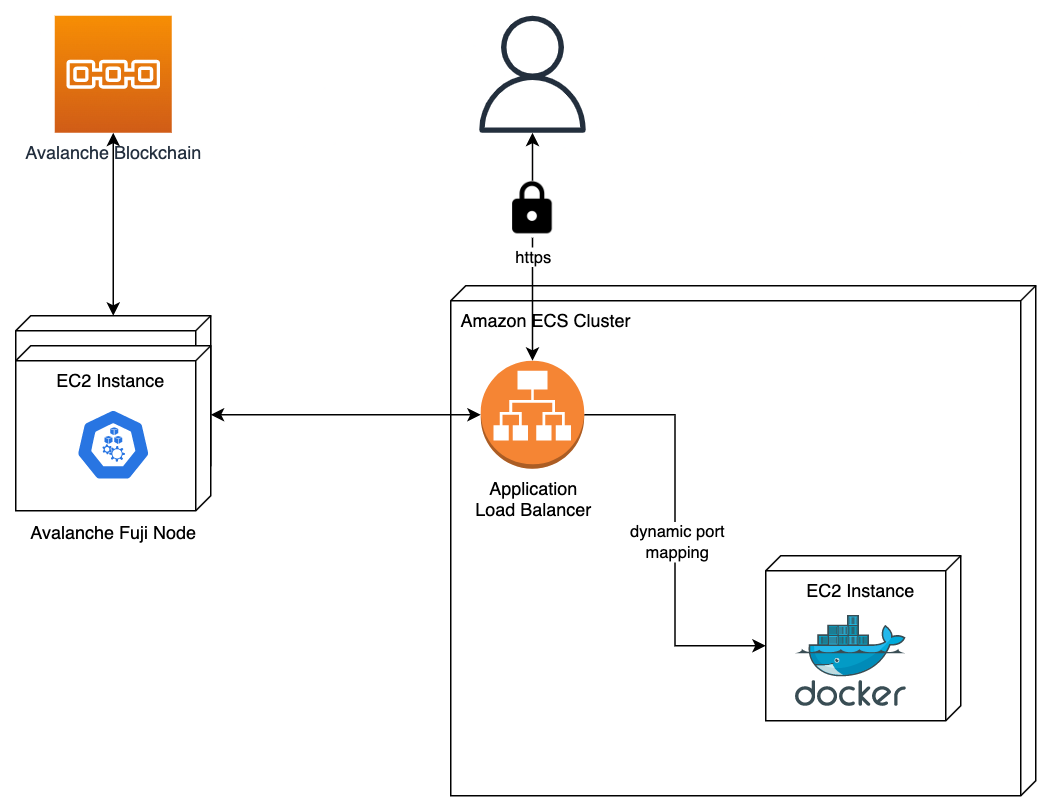
\includegraphics[width=1\textwidth]{deployment.png}
	\caption{Deployment Diagram}
\end{figure}

\chapter{Results}
\section{Evaluation of the Test Results}
The test cases provided were comprehensive and explanatory. All of the 147 tests were successful. Different scenarios were created to simulate and test various user behaviors. Not only the functions themselves were tested but also, the relationships between them were meticulously examined.

Tests were applied for all types of resources, distribution algorithms and allowance options.

In addition to those, gas cost results were satisfactory as well. The functions that depend on the maximum demand volume were able to scale well with the increasing values of it. The differences between the gas costs found in this project and the ones in the paper "Quantized and Simulated Max-min Fairness in Blockchain Ecosystems" [1] were small. Given that the claimBulk() function introduced by us also had feasible gas costs, it can be said that we were able to increase the convenience for the users while not making significant concessions from the scalability. On the contrary, since it first calculates the total share of the user and then sends the transfer only once, it reduces the gas costs in general.
\newpage
\section{Evaluation of the Project}
We have provided a solution for deploying custom subnets and blockchains, and distributing a wide variety of assets on them, utilizing the fair distribution algorithms.

We implemented the two algorithms mentioned in Quantized and Simulated Max-min Fairness in Blockchain Ecosystems [1], namely QMF and SMF, and also provided an Equal Distribution algorithm option that simply distributes the equal share, calculated by simple division, or less. Also, since we used ShareCalculator as a library for these calculations, it is now easier to integrate these distribution algorithms into any blockchain application. It is also easier to observe the functionality of the contracts.

We also built a comprehensive front-end for our blockchain application along with a strong infrastructure. We ran our own node on Avalanche’s testnet Fuji, and provided it as a service for accessing the blockchain for any interaction with Avalanche APIs. Although Metamask does not support the transaction on any other chain except EVM-compatible ones, we were able to come up with a solution and handle the transactions with user signatures. Thanks to this implementation, the users are now able to make transactions on both P and X chain without leaving Metamask wallet.

The utility we are providing is unique and advanced. 

\chapter{Conclusion}
First of all, we were able to deliver a software product that is fully deployed and integrated to blockchain with a decent user interface. Additionally, our smart contracts are tested extensively, deployed and verified on blockchain explorers. We also ran a fully bootstrapped node and validated our subnets and mined blocks for our customized chains. Finally integrating it into our front-end application, we connected separate chains into each other with an interface and node. We believe we were successful, in brief.

Our research has also yielded satisfactory results, gas costs for our implementation were definitely feasible. Using libraries for share calculation operations indeed decreased the gas costs as well.

We built a complex class structure among the distribution contracts so that it could be customized and updated only with a minor change in the base class. It definitely improved the coding style and provided a generalized infrastructure that allows anyone to proceed with our current development later.

Apart from those, our front-end application was also decent given how narrow our time window was. We delivered an enjoyable UI/UX while providing almost the entire functionality of the project. Integrating it with the Avalanche’s X and P chains while only using Metamask was also unique and a great progress.

\newpage 
We also had failures while attempting to integrate more features into our application. One instance of it is integrating the Dominant Resource Fairness algorithm. We started to work on it at the late stages of the development, and the task was more sophisticated than we expected. Integrating the DRF algorithm into a blockchain application was challenging because of the blockchain’s limitations. Then, we decided to allocate our time more efficiently and conceded that feature. On the other hand, our application was very comprehensive and it required many different protocols to work together smoothly making it already a big project.

In conclusion, we are happy with our application and development. It is possible to make improvements and integrate more features in the future thanks to the way the application and the contracts were built.

\chapter{References}
\begin{itemize}
	\item[1.] Metin S., Ozturan C., Quantized and Simulated Max-min Fairness in Blockchain Ecosystems 
	
	\item[2.] Ghodsi A., Zaharia M., Hindman B., Konwinski A., Shenker S., Stoica I., Dominant Resource Fairness: Fair Allocation of Multiple Resource Types
	
	\item[3.] T. Bonald, L. Massouli´e, A. Prouti`ere, J. Virtamo, A Queueing Analysis of Max-Min Fairness,Proportional Fairness and Balanced Fairness
\end{itemize}

\end{document}